\documentclass[11pt,class=report,crop=false]{standalone}
\usepackage[screen]{../python}

%\newcommand{\mot}[1]{\texttt{#1}}

\begin{document}


%====================================================================
\chapitre{ChatGPT -- partie 1}
%====================================================================

% \insertvideo{}{}



\objectifs{Comment est-il possible pour un ordinateur de générer un texte aussi cohérent que des phrases écrites par un humain ? Nous commençons par expliquer le principe général. Puis, partant de statistiques sur les mots d'un texte, nous expliquons les concepts de token et de plongement.}


%%%%%%%%%%%%%%%%%%%%%%%%%%%%%%%%%%%%%%%%%%%%%%%%%%%%%%%%%%%%%%%%%%%%%
\section{Qu'est-ce que \emph{ChatGPT} ?}

Commençons par demander à \emph{ChatGPT} (version 3.5) de \og{}Faire une courte introduction sur le principe de fonctionnement de \emph{ChatGPT} avec l'accent sur les aspects mathématiques.\fg{}
Voici sa réponse :
\begin{center}
\begin{minipage}{0.9\textwidth}
\emph{\og{}
ChatGPT fonctionne grâce à une architecture de réseau de neurones appelée GPT\index{GPT} (Generative Pre-trained Transformer). Cette architecture utilise des opérations linéaires et non linéaires, notamment des couches d'attention, pour traiter l'information. Le modèle est massivement pré-entraîné sur des données textuelles, utilisant des techniques mathématiques avancées telles que la rétropropagation du gradient et l'optimisation par descente de gradient.
\fg{}}
\end{minipage}
\end{center}

C'est une réponse très impressionnante.
Il y a plein de termes que nous connaissons : réseau de neurones, rétropropagation, descente de gradient. Il y a d'autres concepts qu'il va falloir étudier, ce travail va être divisé en deux parties :
\begin{itemize}
  \item la première partie est consacrée aux données textuelles avec les notions de \emph{token} et de \emph{plongement},
  
  \item la seconde partie sera consacrée au type de réseau de neurones adapté aux données textuelles avec les notions de \emph{transformer} et d'\emph{attention}.

\end{itemize}

Le domaine d'étude de la génération automatique de texte s'appelle le \emph{traitement automatique du langage naturel} (NLP, \emph{Natural Language Processing}).
Nous allons nous concentrer sur les LLM\index{LLM} (\emph{Large Language Model}) 
qui ont eu un grand succès ces dernières années grâce à \emph{ChatGPT} et ses variantes.
\emph{ChatGPT} est un robot conversationnel basé sur le modèle de langage \emph{GPT}. Dans ces chapitres nous allons en expliquer le principe général. Pour les exemples, on s’appuiera sur \emph{GPT2} (dont les paramètres sont publiquement accessibles) et sur un autre modèle appelé \emph{BERT}. On construira aussi nous-mêmes des générateurs de textes élémentaires.

	
Ces techniques étant nouvelles et essentiellement développées outre-atlantique nous ne chercherons pas à traduire tous les termes. Par exemple le mot \emph{token}, se traduirait dans notre contexte par \emph{portion} ou bien \emph{tronçon}. De plus, nos exemples linguistiques seront basés sur l'anglais car les ressources sont beaucoup plus facilement accessibles.



%--------------------------------------------------------------------
\subsection{Un exemple de génération de texte}

Demandons à \emph{ChatGPT} (plus précisément à \emph{GPT2}) de continuer la phrase suivante:
\mycenterline{\mot{This dog is ...}}
Le mot le plus probable est \og\mot{a}\fg. On demande donc ensuite à la machine de compléter la phrase 
\mycenterline{\mot{This dog is a ...}}
Le mot le plus probable est \og\mot{great}\fg{} :
\mycenterline{\mot{This dog is a great ...}}
On continue ainsi jusqu'à obtenir une phrase complète :
\mycenterline{\mot{This dog is a great companion}}
\mycenterline{\mot{This dog is a great companion for}}
\mycenterline{\mot{This dog is a great companion for me}}
\mycenterline{\mot{This dog is a great companion for me.}}

En fait, le modèle calcule pour chacun des $50\,000$ tokens la probabilité que ce soit le mot suivant. 
Pour compléter notre phrase \mot{This dog is ...} voici les cinq mots les plus probables : 
\begin{center}
\mot{This dog is}
	\begin{tabular}{|ll}
		\mot{a}  & 11.8 \% \\
		\mot{very}   & 4.7 \% \\
		\mot{not}   & 3.6 \% \\
		\mot{so}   & 2.9 \% \\
		\mot{an} & 2.2 \% \\
	\end{tabular}
\end{center}
Une fois que le \og\mot{a}\fg{} a été choisi, on calcule les nouvelles probabilités pour le mot suivant :
\begin{center}
	\mot{This dog is a}
	\begin{tabular}{|ll}
		\mot{great}  & 4.5 \% \\
		\mot{very}   & 4.0 \% \\
		\mot{good}   & 3.0 \% \\
		\mot{bit}   & 2.8 \% \\
		\mot{little} & 1.8 \% \\
	\end{tabular}
\end{center}

Pour construire des phrases plus variées, on utilise un paramètre appelé \emph{température} qui contrôle la variabilité de la complétion. Prenons par exemple à chaque itération, le troisième mot le plus probable, on obtient :
\mycenterline{\mot{This dog is not going away.}}

\medskip
	
La variante de \emph{GPT} la plus célèbre est bien sûr \emph{ChatGPT}, dont la fonction principale est de répondre à des questions. Mais en y regardant de plus près, cette capacité n'est pas vraiment éloignée de celle que nous avons discutée : répondre à la question \mot{What's this dog ?} revient à savoir compléter la phrase \mot{This dog is ...}, c'est à dire compléter la forme affirmative de la question posée.


%--------------------------------------------------------------------
\subsection{Principe général}

Voici les grandes étapes qui seront étudiées dans ce chapitre ainsi que le suivant afin de compléter une phrase.

\begin{itemize}
	\item \textbf{Tokenisation.} 
	Il s'agit de découper un texte en une suite de mots ou de parties de mots, appelés \emph{tokens}. Chaque token est codé par un numéro. (Il y a $N=50\,257$ tokens pour \emph{GPT2}.)
	
	\item \textbf{Plongement.} (\emph{Embedding.})
	Chaque token (ou chaque mot si vous préférez) est transformé en un vecteur de très grande taille. (Pour \emph{GPT2} un vecteur token $v$ est un vecteur de  $\Rr^n$ avec $n=768$.) De plus, on fait en sorte que dans ce vecteur soit aussi encodée la position du token dans la phrase.
	Ainsi une phrase (composée de $K$ tokens) est codée par une liste de vecteurs $(v_1,v_2,\ldots,v_K)$,	c'est-à-dire par une matrice $M \in M_{n,K}$ ($n$ lignes, $K$ colonnes).
	
	\item \textbf{Retranscription.} (\emph{Unembedding.})
	À la fin, en sortie du réseau, on obtient un vecteur $w \in \Rr^n$. On pourrait chercher parmi les $N= 50\,257$ vecteurs tokens, lequel est le plus proche (la distance entre deux vecteurs est définie par le produit scalaire ou la \emph{similarité cosinus}). On préfère attribuer une probabilité de correspondance à chacun des $N$ tokens et, par exemple, choisir le mot suivant parmi les $10$ plus probables.
	
	\item \textbf{Transformeur.} (\emph{Transformer.}) L'architecture des réseaux de neurones pour les grands modèles de langage (LLM) se nomme transformeur. En son c\oe ur on trouve deux types de couches. Le premier type est simplement composé de couches denses de neurones (MLP, \emph{Multi Layer Perceptron}, sans convolution) comme on a déjà rencontrées dans les chapitres précédents. 
	
	\item \textbf{Attention.} 
	Les couches de second type sont les couches d'attention qui ont fait le succès des LLM après l'article fondateur \emph{Attention is all you need} par une équipe de \emph{Google}. 
	Dans une phrase tous les mots n'ont pas la même importance pour comprendre son sens. L'attention consiste à attribuer des poids aux mots en fonction de leur pertinence dans la phrase. Par exemple, en oubliant les articles ou les adjectifs inutiles, afin de mettre en évidence la structure sujet/verbe/complément.
	En fait à chaque mot/token de la phrase on associe une liste des poids aux autres mots de la phrase qui explique le sens du mot dans cette phrase. 	
	On détaillera le mécanisme d'attention dans le chapitre suivant.
	
	\item \textbf{Réseau.}
	Le réseau est gigantesque. Par exemple, le modèle \emph{GPT2-Small} que l'on étudiera possède $117$ millions de poids. Il est composé de $24$ couches : $12$ couches de neurones et $12$ couches d'attention (chacune avec $12$ têtes d'attention). Mais surtout ce réseau est entraîné sur un corpus gigantesque basé sur plusieurs gigaoctets de documents (livres, articles, pages web, forum\ldots) principalement en anglais. 
	Le paramétrage du réseau nécessite énormément de calculs, il est donc indispensable de posséder des algorithmes performants, des ordinateurs puissants travaillant en parallèle avec en leur c\oe ur des processeurs graphiques (GPU) adaptés à ce type de calculs.
	
	\item \textbf{Flux résiduel.}
	En plus de l'attention, il y a une différence importante avec les réseaux des chapitres précédents : le flux résiduel (\emph{residual stream}). L'idée est de garder la mémoire de ce que chaque couche a appris afin que toutes les couches suivantes (même les couches éloignées) aient un accès direct aux résultats importants déjà obtenus. Les données envoyées d'une couche à l'autre sont déterminées par les coefficients de matrices qui sont des paramètres du réseau.
	Le flux résiduel remédie en particulier à un problème des réseaux ayant beaucoup de couches pour lesquels la rétropropagation modifie très lentement les poids des premières couches.
	
	\item \textbf{Dimensions.}
	Une des particularité de LLM est de travailler avec des espaces de grandes dimensions (par exemple dans $\Rr^{768}$ pour \emph{GPT2}), cela permet d'avoir \og{}de la place\fg{}, le réseau peut ainsi se réserver des sous-espaces pour envoyer des informations d'une couche à l'autre via le flux résiduel. La contrepartie est que le nombre de poids du réseau devient gigantesque.
	
	
\end{itemize}

	
% Bien sûr ces poids sont calculés par apprentissage et il est toujours délicat d'expliquer ce que fait précisément l'attention ou le réseau. Ce qui est visible, est que cela fonctionne en construisant des phrases pertinentes.

%--------------------------------------------------------------------
\subsection{Architecture du réseau}

Voici l'architecture de \emph{GPT2-Small} dont le modèle est publiquement accessible ainsi que ses poids après entraînement.

\begin{itemize}
	\item Nombre de tokens $N = 50\,257$.
	\item Dimension de plongement $n=768$.
	\item Une phrase est découpée en $K = 1024$ tokens maximum.
	\item Nombre de couches d'attention : $12$ (avec chacune $12$ têtes d'attention).
	\item Nombre de couches denses : $24$ ($12$ fois une paire de couches).
	\item Nombre total de poids du réseau : $117$ millions.
	\item Entraîné sur un corpus de plusieurs dizaines de gigaoctets de textes variés.
\end{itemize}

Ci-dessous à gauche l'architecture globale du réseau, et à droite plus de détails pour la partie \og{}transformeur\fg{} qui est le c\oe ur du réseau.

\begin{center}
\begin{minipage}{0.49\textwidth}
\small	
\myfigure{0.7}{
	\tikzinput{gpt-01}
}
\end{minipage}
\begin{minipage}{0.49\textwidth}
		
	\myfigure{0.6}{\footnotesize
		\tikzinput{gpt-02}
	}
\end{minipage}
\end{center}


Depuis, les progrès ont été constants. Les réseaux sont de plus en plus grands (avec plusieurs milliards de poids), entraînés dans toutes les langues possibles (y compris les langages informatiques). Ils peuvent être spécialisés (\emph{fine tuning}) pour répondre à une tâche spécifique (assistance internet, classification de documents, génération de code \Python\ldots). Nul doute qu'ils vont encore beaucoup progresser.

Notre modeste but est de comprendre le principe de fonctionnement global en donnant un nombre raisonnable de détails. Le travail s'étend sur deux chapitres. Il suppose la connaissance des couches denses de neurones.


%%%%%%%%%%%%%%%%%%%%%%%%%%%%%%%%%%%%%%%%%%%%%%%%%%%%%%%%%%%%%%%%%%%%%
\section{Statistique et linguistique}

Nous allons voir comment l'étude des fréquences des mots dans les textes permet de générer des phrases qui ressemblent à des phrases cohérentes.

%--------------------------------------------------------------------
\subsection{La loi de Zipf-Mandelbrot}

Commençons par étudier la fréquence des mots dans un (grand) texte.
Prenons un ensemble de dépêches de l'agence \emph{Reuters}\index{donnees@données!Reuters} qui fournit des informations économiques et politiques. Ce \emph{corpus} est constitué de plus de $10\,000$ dépêches en anglais qui forment un total de plus de $1.7$ millions de mots.
Voici un extrait :
\mycenterline{
\emph{The country's oil import bill, however, fell 23 pct in the first quarter due to lower oil prices.}}

Voici les $10$ mots (de deux lettres ou plus) les plus fréquents et leur nombre d'occurrences :

\begin{center}
\begin{tabular}{ll}
\mot{the}  & 58251 \\
\mot{of}   & 35979 \\
\mot{to}   & 34035 \\
\mot{in}   & 26478 \\
\mot{said} & 25224 \\
\end{tabular}
\qquad\qquad
\begin{tabular}{ll}
\mot{and}  & 25043 \\
\mot{mln}  & 18037 \\
\mot{vs}   & 14120 \\
\mot{for}  & 12785 \\
\mot{dlrs} & 11730 \\
\end{tabular}
\end{center}
Voici le graphique des nombres d'occurrences des $50$ mots les plus fréquents.
\begin{center}
	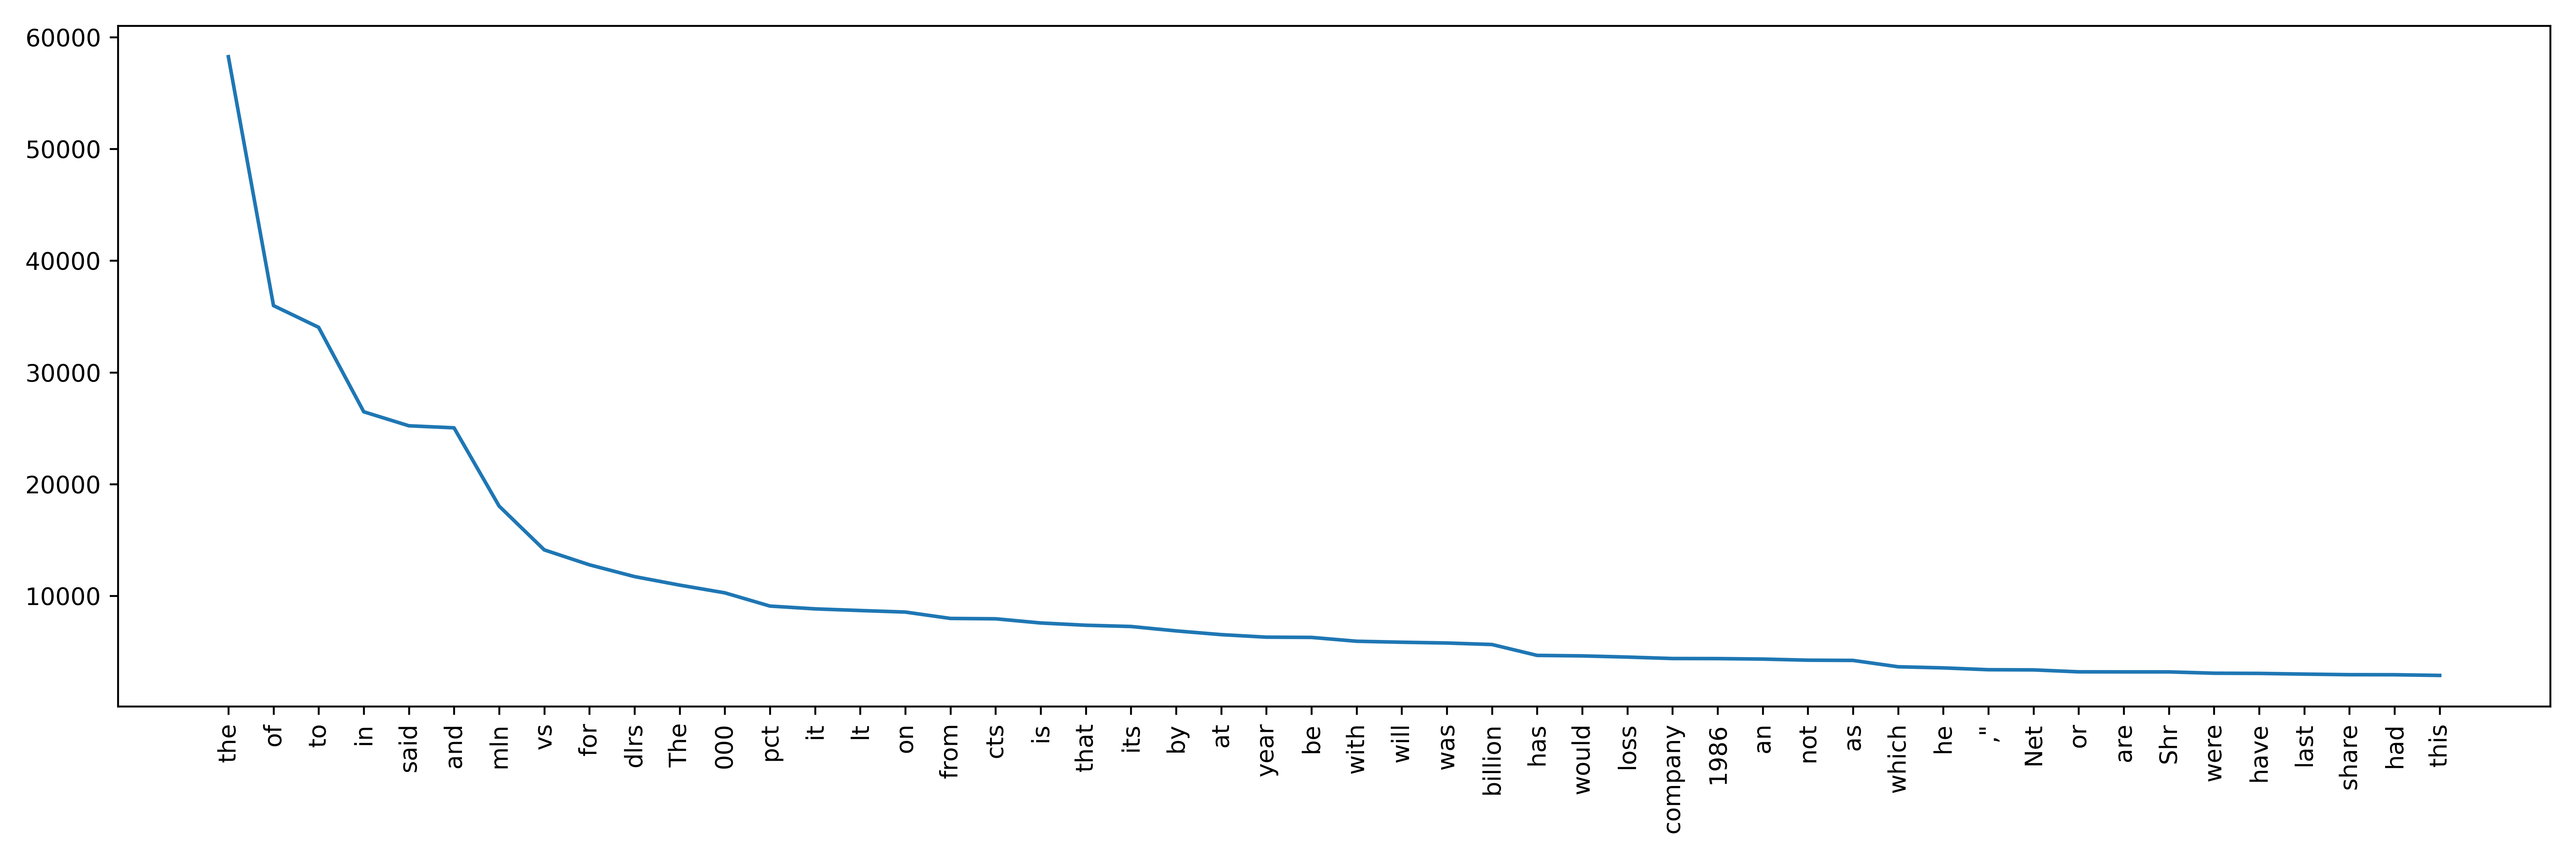
\includegraphics[scale=\myscale,scale=0.45]{figures/linguistique-01}
\end{center}


Quelle formule régit ce nombre d'occurrences ?
Une règle simple que l'on constate est que si le mot le plus fréquent apparaît $N$ fois, alors le deuxième mot le plus fréquent apparaît $N/2$ fois, le troisième mot le plus fréquent $N/3$\ldots{} Ainsi la répartition des occurrences en fonction du rang se fait selon les termes :
\[ 1 \qquad \frac12 \qquad \frac13 \qquad \frac14 \qquad \ldots \]
Cette observation expérimentale se retrouve dans n'importe quel grand texte, quelle que soit sa langue.
Elle se décline avec plus de précision dans la \defi{loi de Zipf-Mandelbrot}\index{loi de Zipf-Mandelbrot}:
\[ f_i = \frac{a}{(i+b)^c} \]
où :
\begin{itemize}
	\item $i \ge 1$ est le rang du mot concerné,
	\item $f_i$ est sa fréquence (c'est-à-dire le nombre d'occurrences du mot divisé par le nombre total de mots),
	\item $a,b,c$ sont des constantes réelles à déterminer (avec $c \simeq 1$).
\end{itemize}

Pour nos dépêches, voici le graphique des $200$ premières occurrences ainsi que le graphe de la fonction $x \mapsto \frac{a}{(b+x)^c}$ avec ici  $a=0.1$, $b=1.5$, $c=0.95$:

\begin{center}
	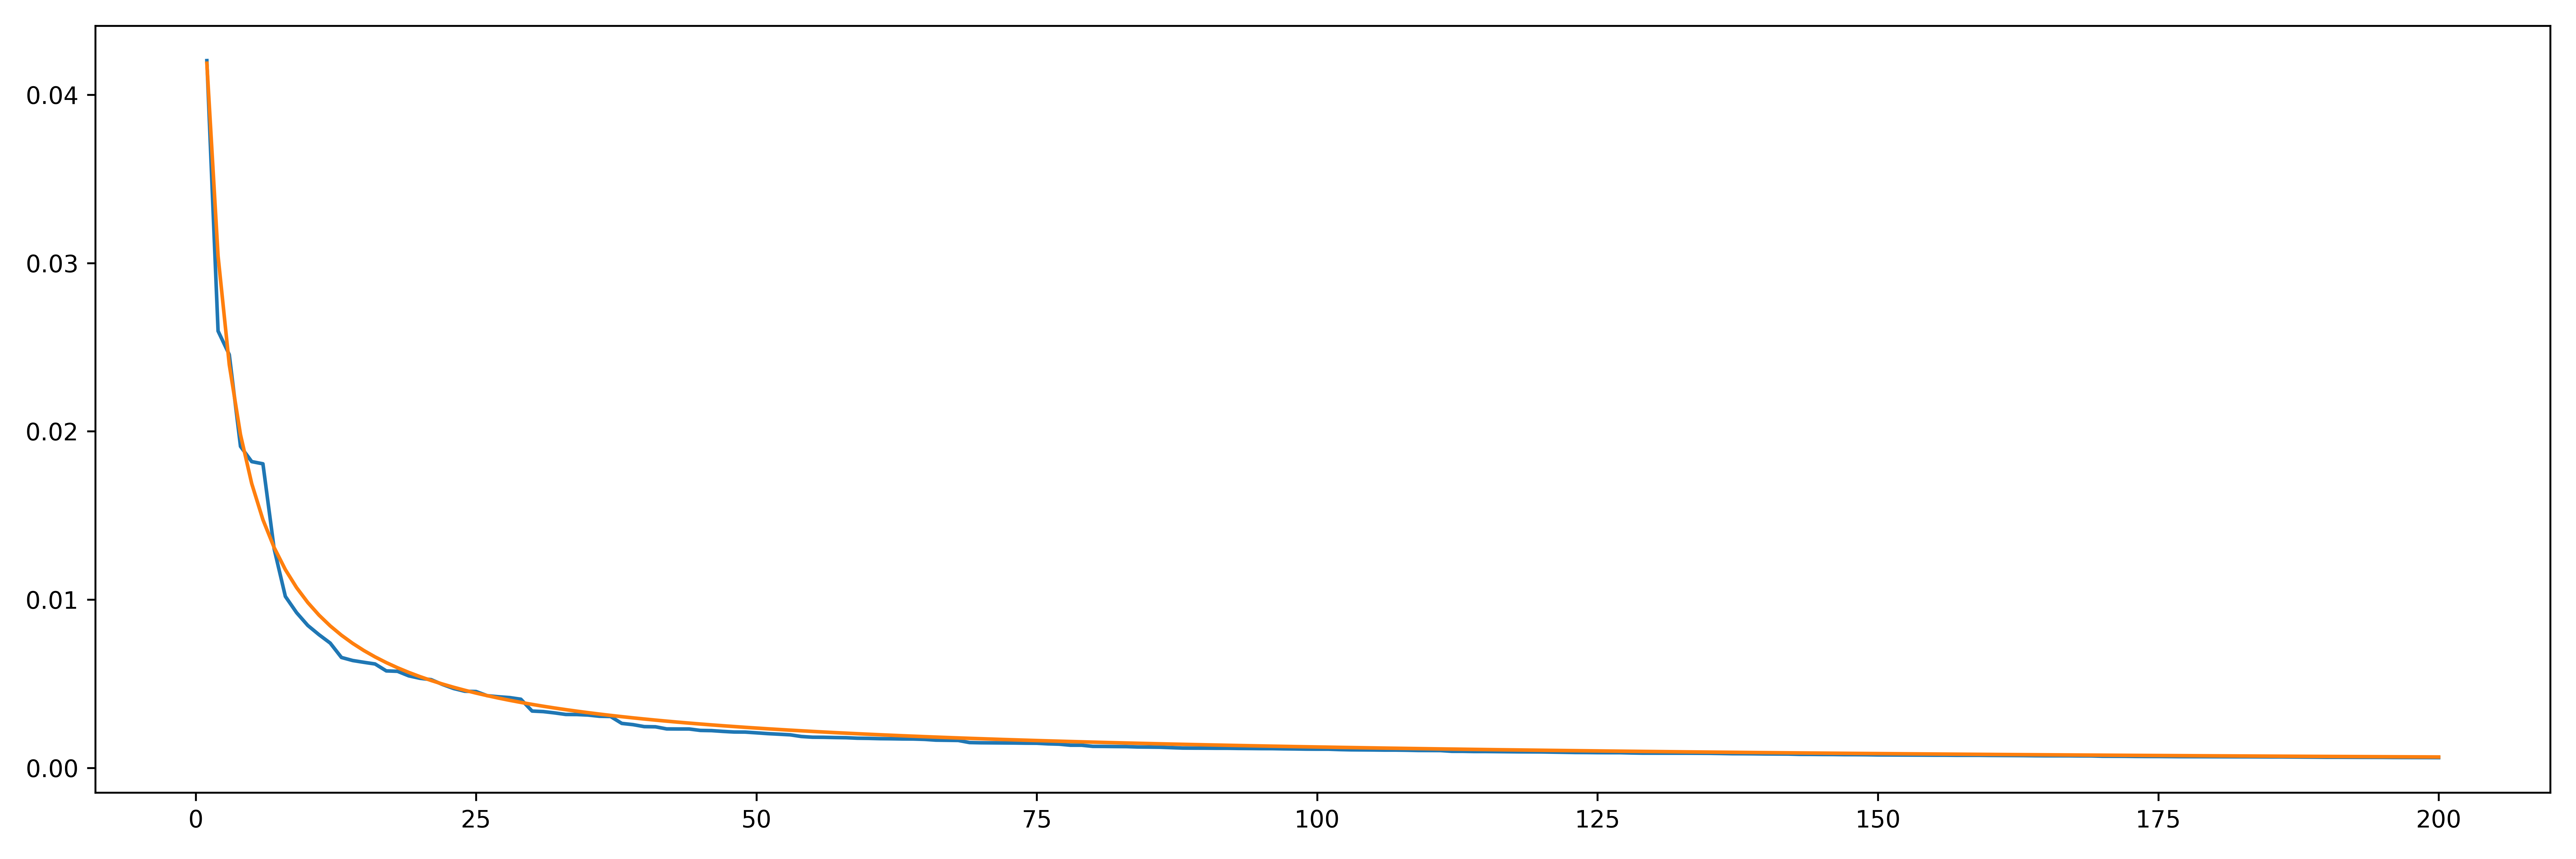
\includegraphics[scale=\myscale,scale=0.4]{figures/linguistique-02}
\end{center}

Il est plus facile de visualiser l'ajustement en utilisant une échelle logarithmique (ici sur les $500$ mots les plus fréquents).

\begin{center}
	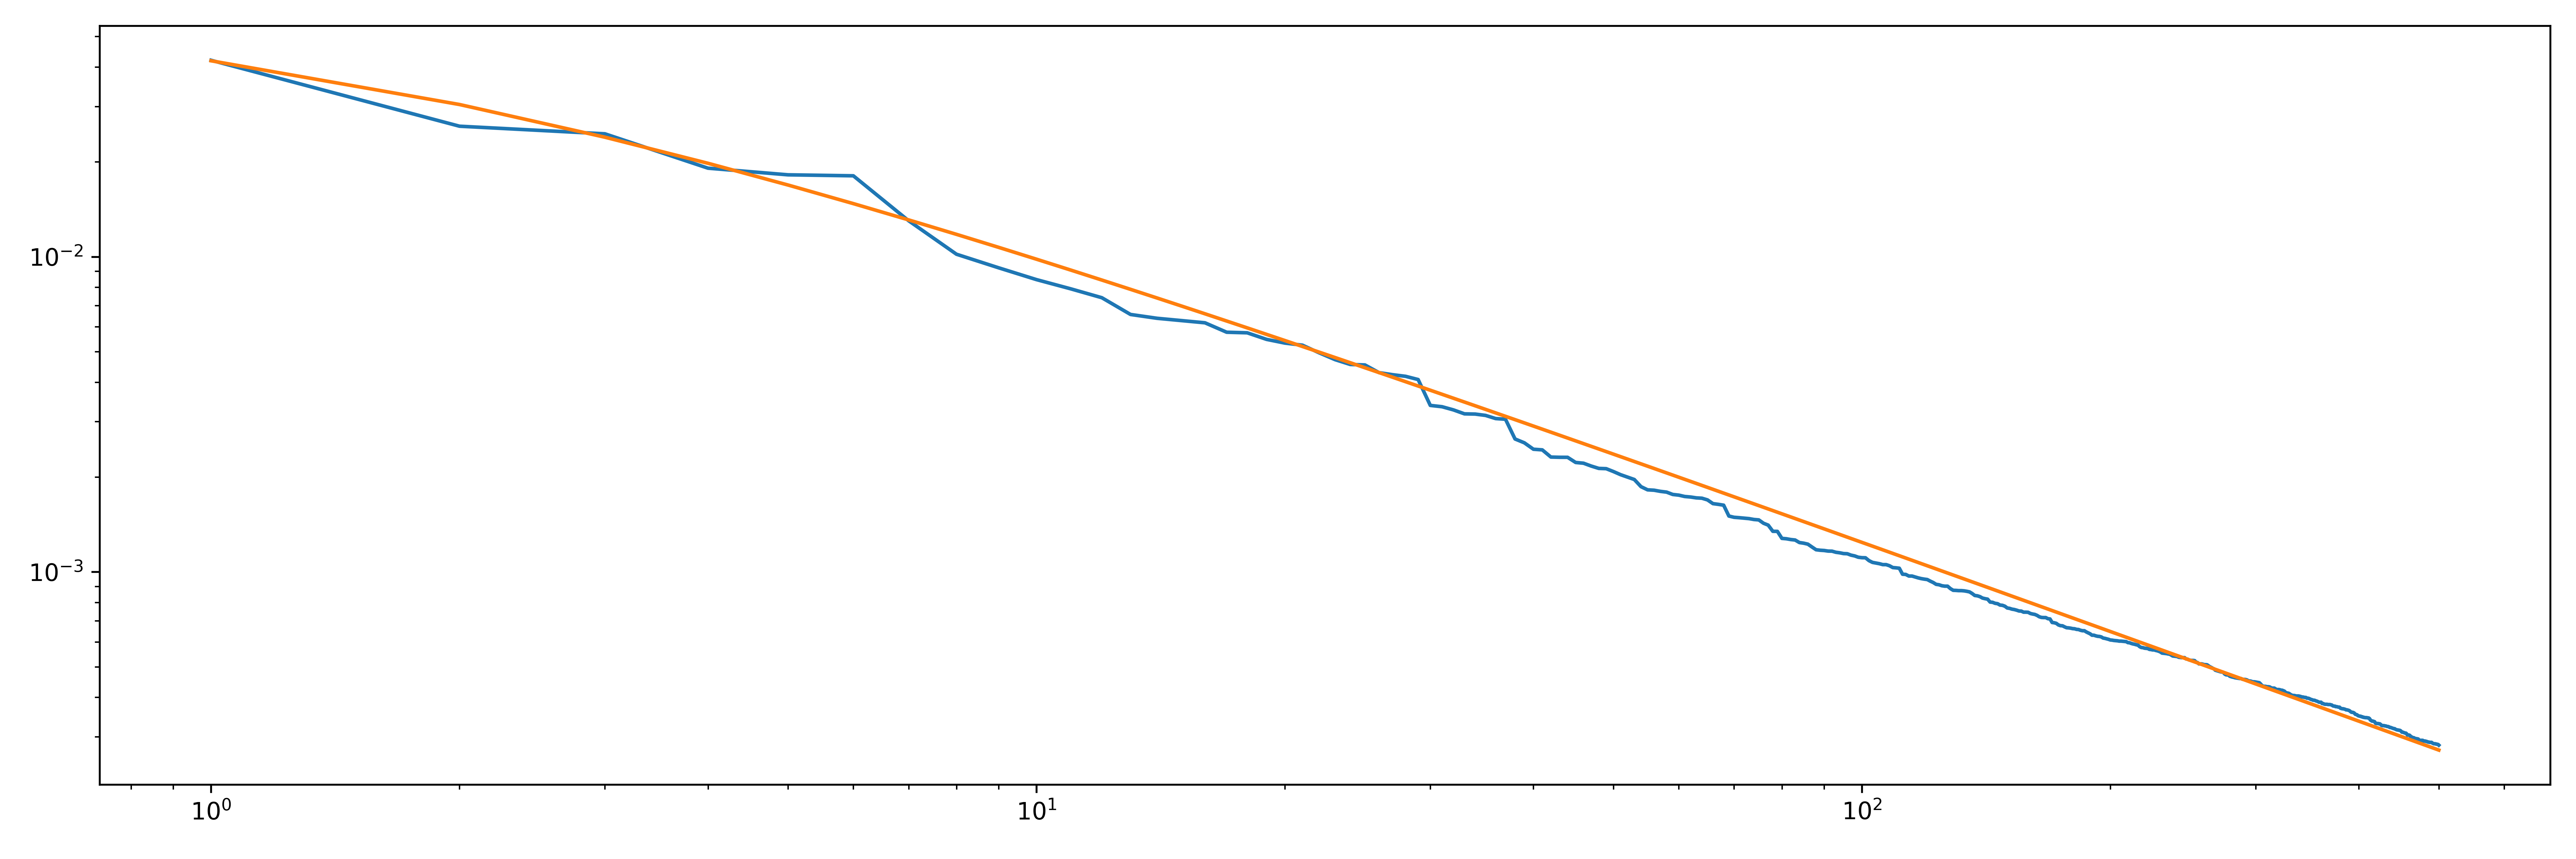
\includegraphics[scale=\myscale,scale=0.4]{figures/linguistique-03}
\end{center}
En effet si $y = \frac{a}{(b+x)^c}$ alors 
$\ln(y) = \ln(a) - c \ln(b+x)$, en posant $Y = \ln(y)$ et $X = \ln(b+x)$ on trouverait l'équation $Y = \ln(a) - cX$ d'une droite. Comme nous traçons $\ln(y)$ en fonction de $\ln(x)$ (et pas de $\ln(b+x)$) nous n'obtenons pas exactement le tracé d'une droite.

Retenons que les mots d'un texte n'apparaissent pas tous avec la même fréquence et que la loi de Zipf-Mandelbrot est une formule empirique qui modélise ces fréquences.


%--------------------------------------------------------------------
\subsection{Co-occurrence}

La fréquence des mots d'une langue ne permet pas de générer des phrases qui paraissent naturelles. Par contre, compter les paires de mots consécutifs va nous permettre de générer des phrases pseudo-naturelles.

La \defi{co-occurrence}\index{co-occurrence} d'une paire de mot (mot1, mot2) est le nombre de fois où mot1 est immédiatement suivi de mot2 dans un texte.
Plus généralement la co-occurrence de (mot1, mot2, \ldots, mot$n$) est le nombre de fois où ces mots apparaissent en se suivant et dans cet ordre.

Par exemple dans les dépêches précédentes, voici les co-occurrences les plus fortes lorsque le premier mot est \mot{the} :
\begin{center}
	\begin{tabular}{lc}
		(\mot{the},\ \mot{company})     & 1941 \\
		(\mot{the},\ \mot{dollar})      & 878  \\		
		(\mot{the},\ \mot{first})       & 810  \\
		(\mot{the},\ \mot{year})        & 704  \\
		(\mot{the},\ \mot{government})  & 620  \\				
	\end{tabular}
\end{center}

Cela nous donne une méthode simple permettant de générer une phrase :
partant d'un premier mot mot1, on choisit pour deuxième mot celui qui 
a la plus grande co-occurrence (mot1, mot2). Puis on choisit le mot suivant réalisant la plus grande co-occurrence (mot2, mot3)\ldots{} On s'arrête lorsque la phrase atteint la longueur voulue.

En commençant par \mot{the} on obtient la phrase :
\mycenterline{
\mot{the company said it has been made by the company}
}


%--------------------------------------------------------------------
\subsection{Softmax et température}

Pour générer des phrases variées et naturelles nous allons ajouter un peu d'aléatoire lors de leur construction. Au lieu de choisir comme mot suivant le plus probable, on peut choisir le mot suivant au hasard, disons parmi les $10$ plus probables.

La façon la plus évidente de le faire est de calculer les $10$ co-occurrences les plus fortes et de choisir un mot au hasard, mais en tenant compte des fréquences. De sorte que, par exemple, après \mot{the}, le mot \mot{company} a deux fois plus de chance d'être choisi que \mot{dollar}.

Voici quelques phrases commençant par \mot{the} que l'on obtient par ce processus aléatoire pondéré :
\mycenterline{\mot{
the end of the company also said it raised to the end assets to acquire		
}}
\mycenterline{\mot{
the United States to the world prices will meet the company said it agreed		
}}
\mycenterline{\mot{
the same month earlier reported 1986 results include nonrecurring costs		
}}
Ces phrases n'ont pas de sens mais elles possèdent quand même une tonalité familière.


\bigskip

Nous allons voir une façon de procéder un peu plus sophistiquée.
Revenons d'abord sur la fonction softmax\index{softmax}.
Pour $X = (x_1,x_2,\ldots,x_k)$ on note :
$$\sigma_i(X)  = \frac{e^{x_i}}{ e^{x_1} + e^{x_2} + \cdots + e^{x_k}}.$$



On définit alors la fonction $\operatorname{softmax}$ par :
$$\begin{array}{rcl}
	\operatorname{softmax} \colon \Rr^k & \longrightarrow & [0,1]^k \subset \Rr^k \\
	X &\longmapsto & \big(\sigma_1(X), \sigma_2(X), \dots, \sigma_k(X)\big)
\end{array}
$$

On a $\sigma_1(X) + \sigma_2(X) + \cdots + \sigma_k(X) = 1$.
On peut donc interpréter les $\sigma_i(X)$ comme des probabilités.
La composante \(\sigma_i(X)\) est d’autant plus grande que \(x_i\) est grand, car la fonction exponentielle amplifie les différences.  
Ainsi, la plus grande valeur parmi les \(\sigma_i(X)\) est atteinte pour l’indice \(i\) tel que \(x_i\) est maximal.
Il s'agit d'une version \og{}lisse\fg{} de la fonction argmax\index{argmax} (on rappelle que la fonction argmax renvoie le rang pour lequel le maximum est atteint).

Nous prenons ici \(X = (x, 1 - x)\) pour visualiser le comportement de la fonction softmax dans un cas simple à deux composantes qui varient de manière complémentaire.
Voici le graphe de $\sigma_1(x) = \frac{e^x}{e^x+e^{1-x}}$ pour $x \in \Rr$.
\begin{center}
	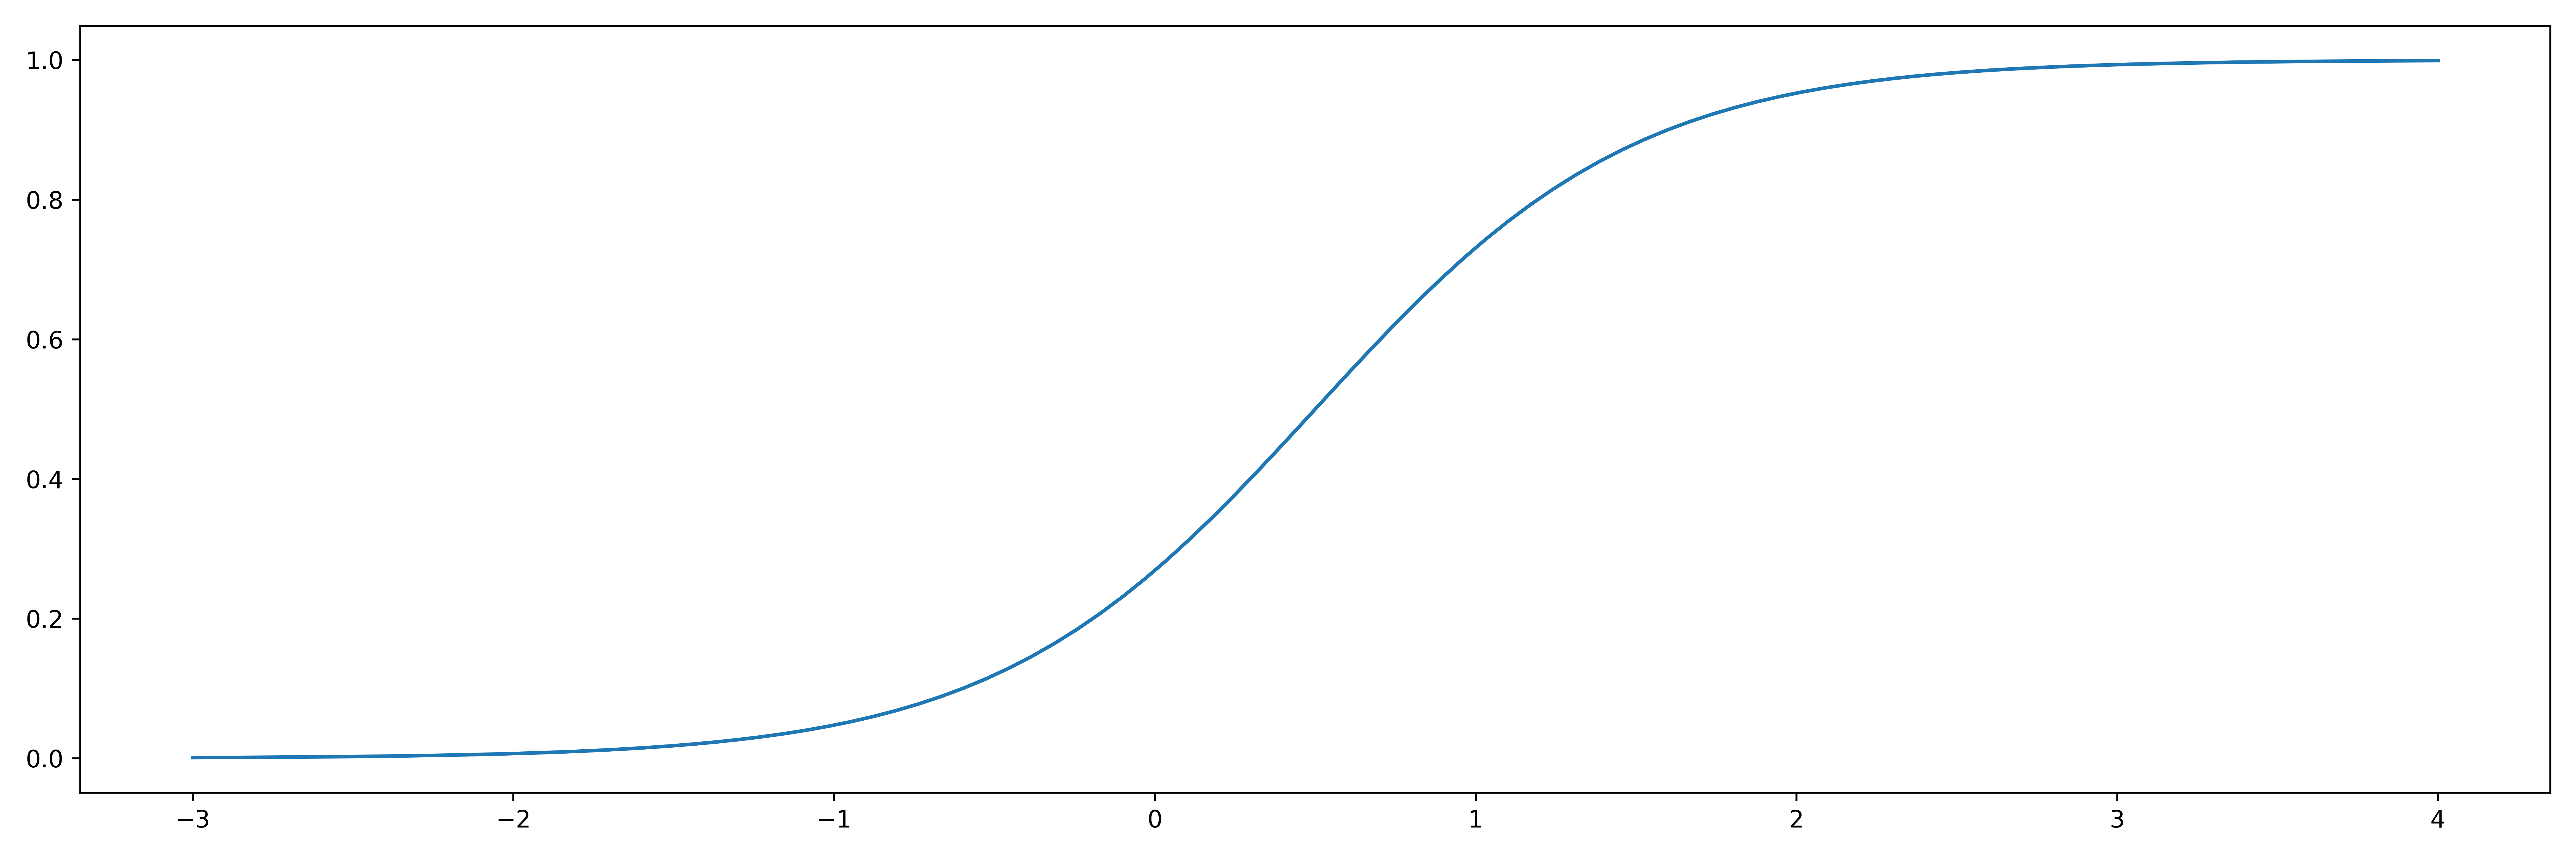
\includegraphics[scale=\myscale,scale=0.4]{figures/softmax-01}
\end{center}

\bigskip

Nous allons rajouter un paramètre, appelé \defi{température}\index{temperature@température}, à la fonction softmax.
Pour $X = (x_1,x_2,\ldots,x_k)$ et $T > 0$, on note :
$$\sigma_{T,i}(X)  = \frac{e^{x_i/T}}{ e^{x_1/T} + e^{x_2/T} + \cdots + e^{x_k/T} }.$$
On a de nouveau $\sigma_{T,1} + \sigma_{T,2} + \cdots + \sigma_{T,k} = 1$.
Et on définit une fonction
$\operatorname{softmax}_T : \Rr^k \to [0,1]^k$, par 
$\operatorname{softmax}_T(X) = \big(\sigma_{T,1}(X), \dots, \sigma_{T,k}(X)\big)$.


Voici les graphes de $\sigma_{T,1}(x) = \frac{e^{x/T}}{e^{x/T}+e^{{1-x}/T}}$ pour $X = (x,1-x)$ et quelques valeurs de $T$.

\begin{center}
	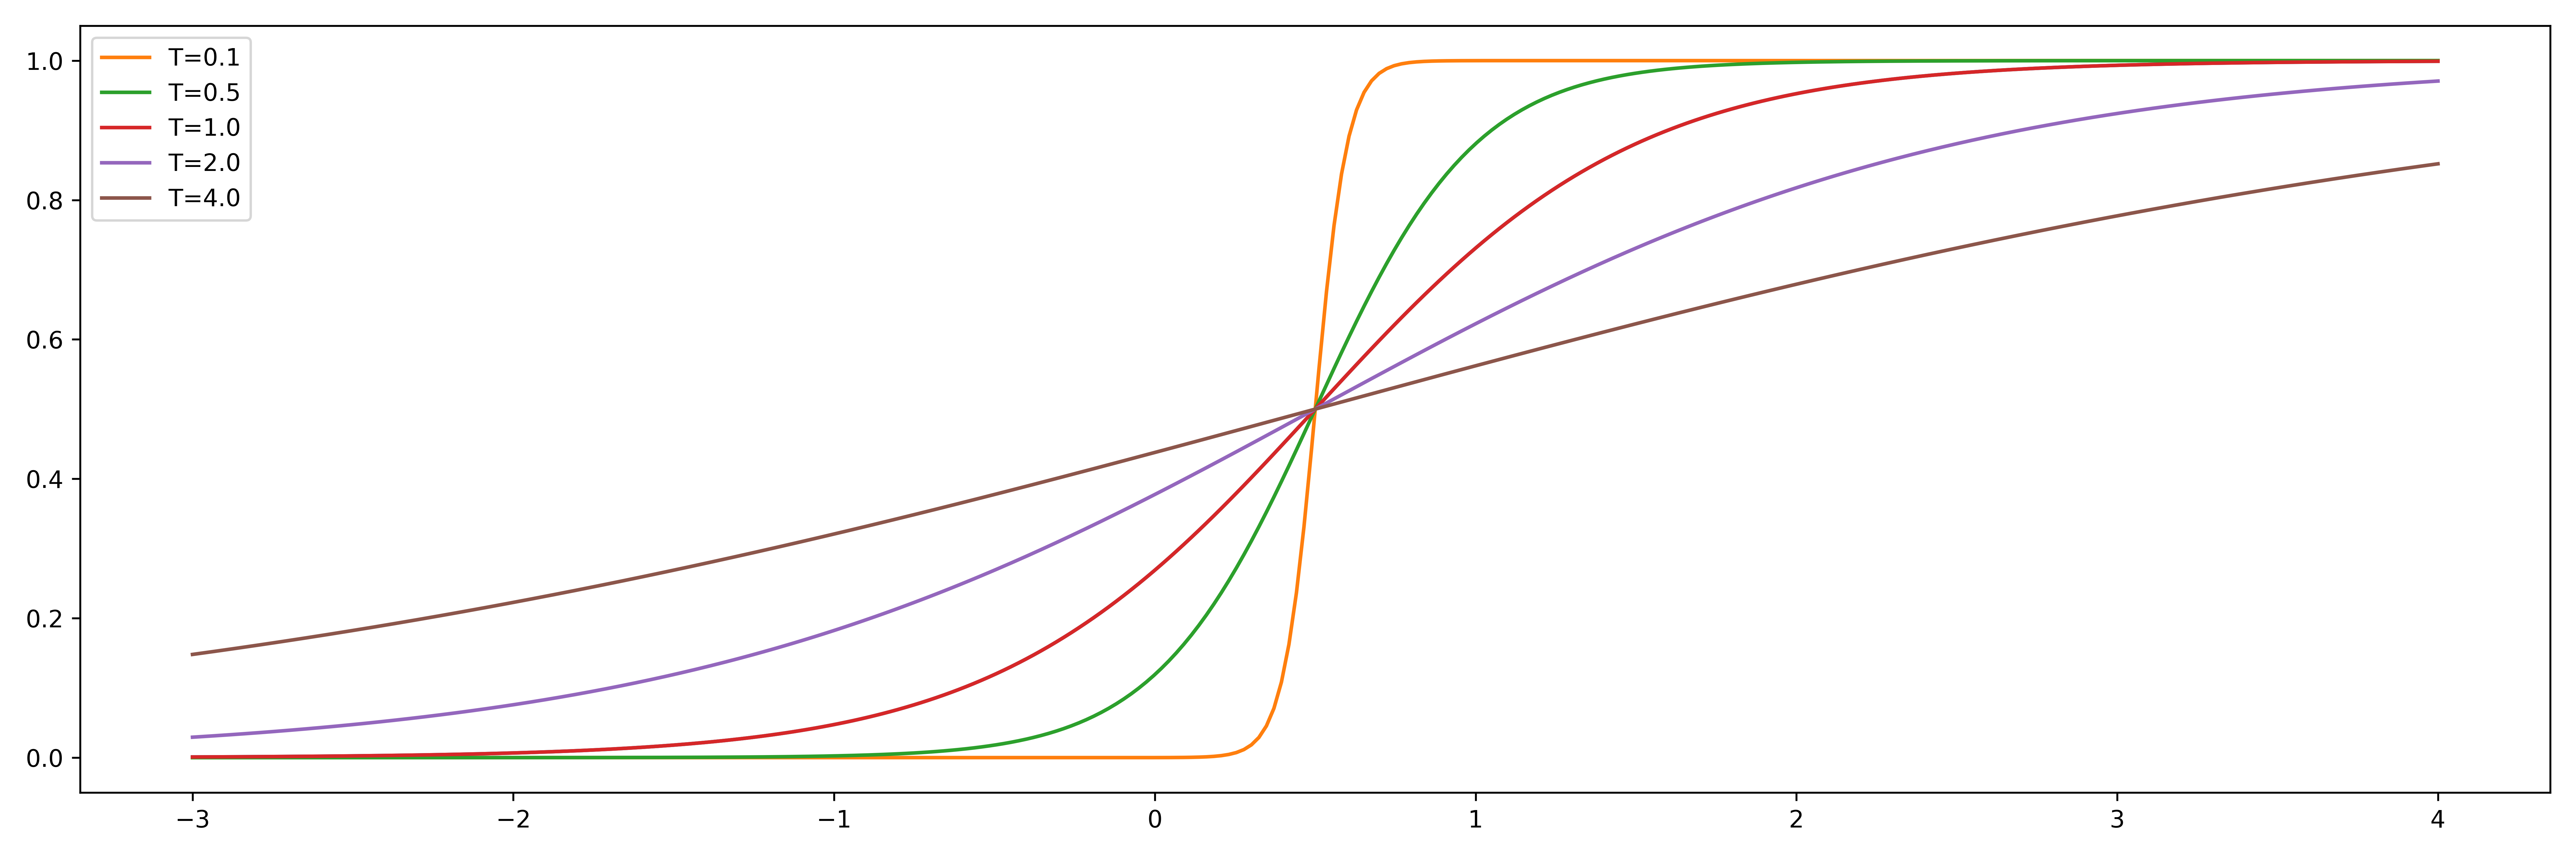
\includegraphics[scale=\myscale,scale=0.4]{figures/softmax-02}
\end{center}

Plus la température est proche de $0$, plus la fonction softmax se rapproche de ce que ferait une fonction argmax, c'est-à-dire que $\sigma_{T,i}$ vaut $1$ là où $x_i$ est le plus grand et $0$ ailleurs.
Plus la température est élevée, plus la fonction softmax se rapproche d'une distribution uniforme, c'est-à-dire $\sigma_{T,i} \simeq \frac 1k$ (quelles que soient les valeurs $x_1,\ldots,x_k$).

Voici un exemple de distribution aléatoire $X = (x_1,x_2,\ldots,x_6) = \frac{1}{53}(2,5,25,3,14,4)$.
\begin{center}
	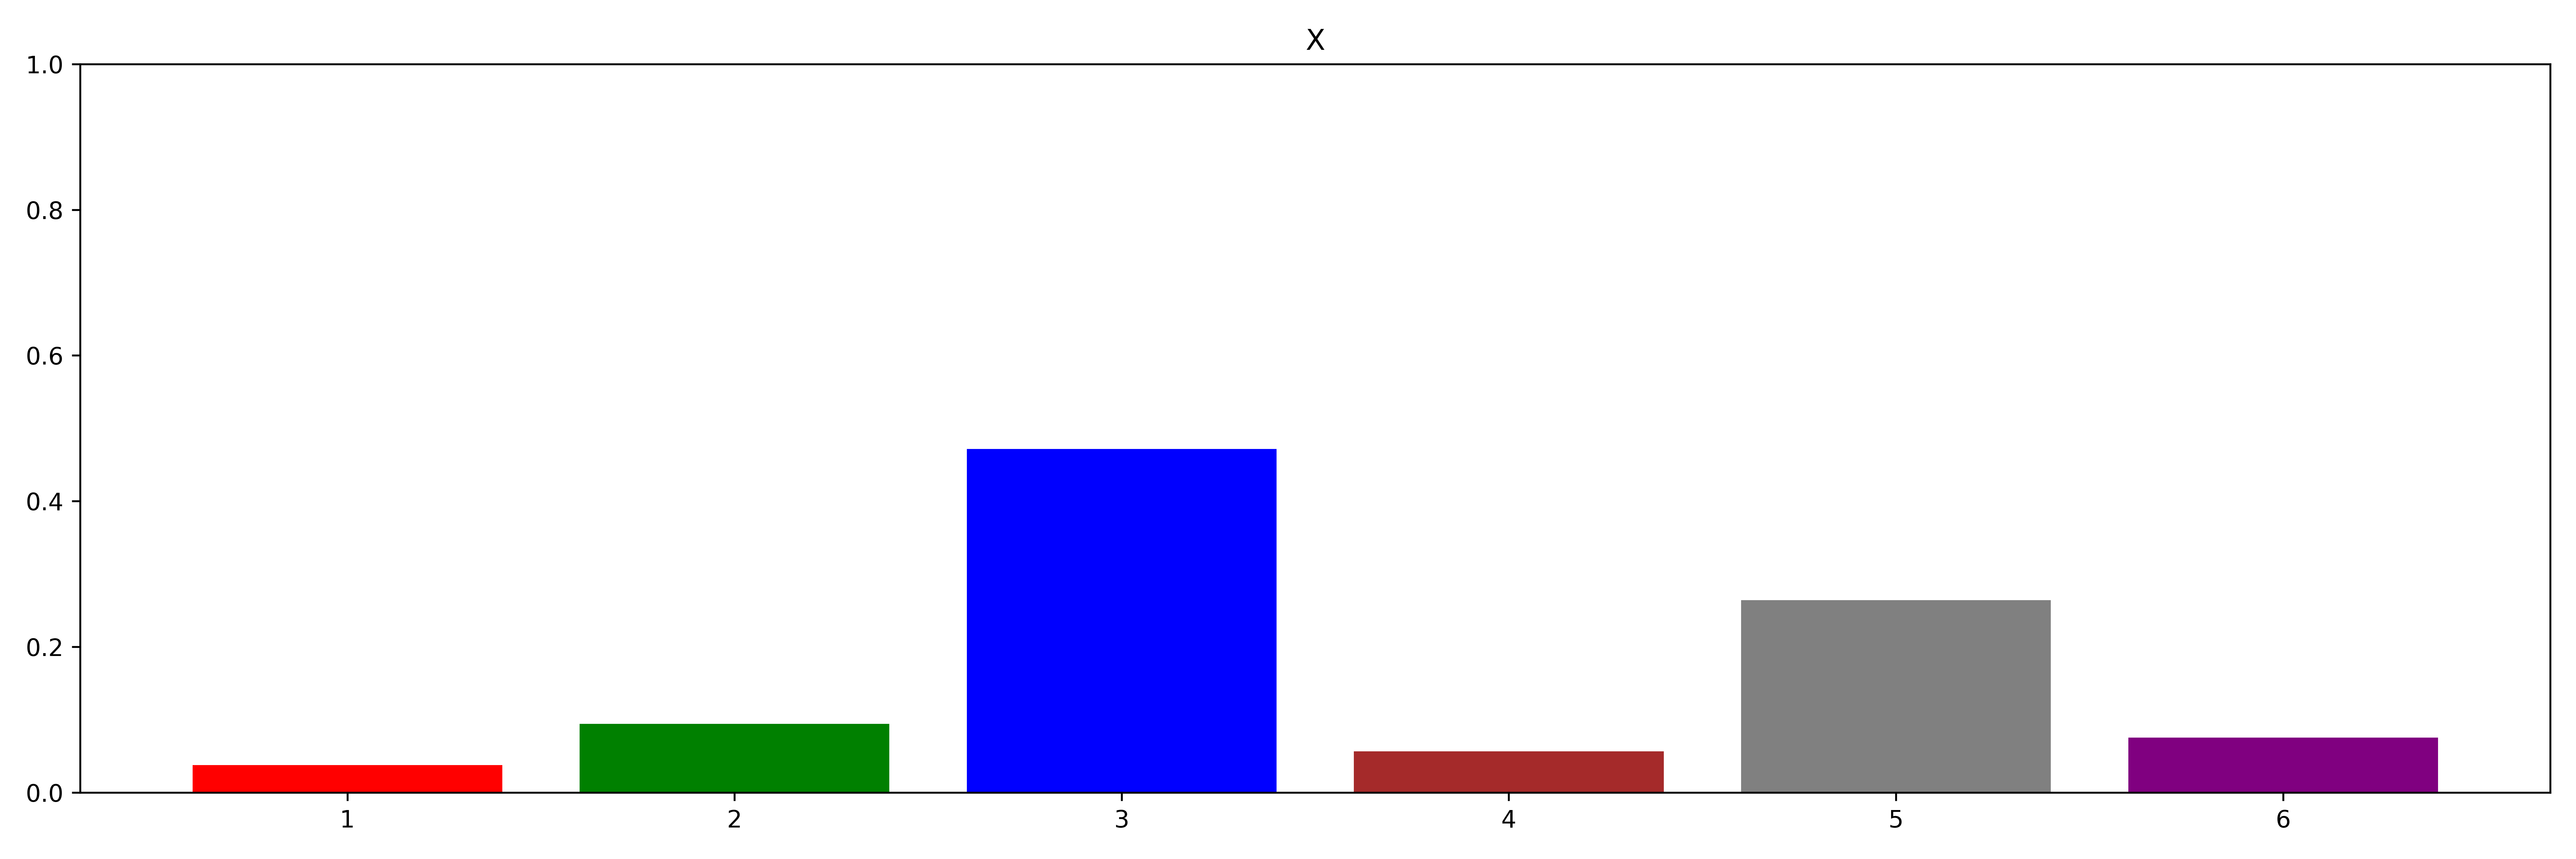
\includegraphics[scale=\myscale,scale=0.4]{figures/softmax-03}
\end{center}

Voici les valeurs renvoyées par $\sigma_{T,i}(X)$ pour différentes températures. Pour $T=0.1$ la valeur $x_i$ la plus élevée est renforcée. Pour $T=0.2$ on retrouve ici à peu près la distribution originale. Pour $T=1$ ou $T=5$ les valeurs retournées correspondent à des distributions quasi-uniformes. 
\begin{center}
	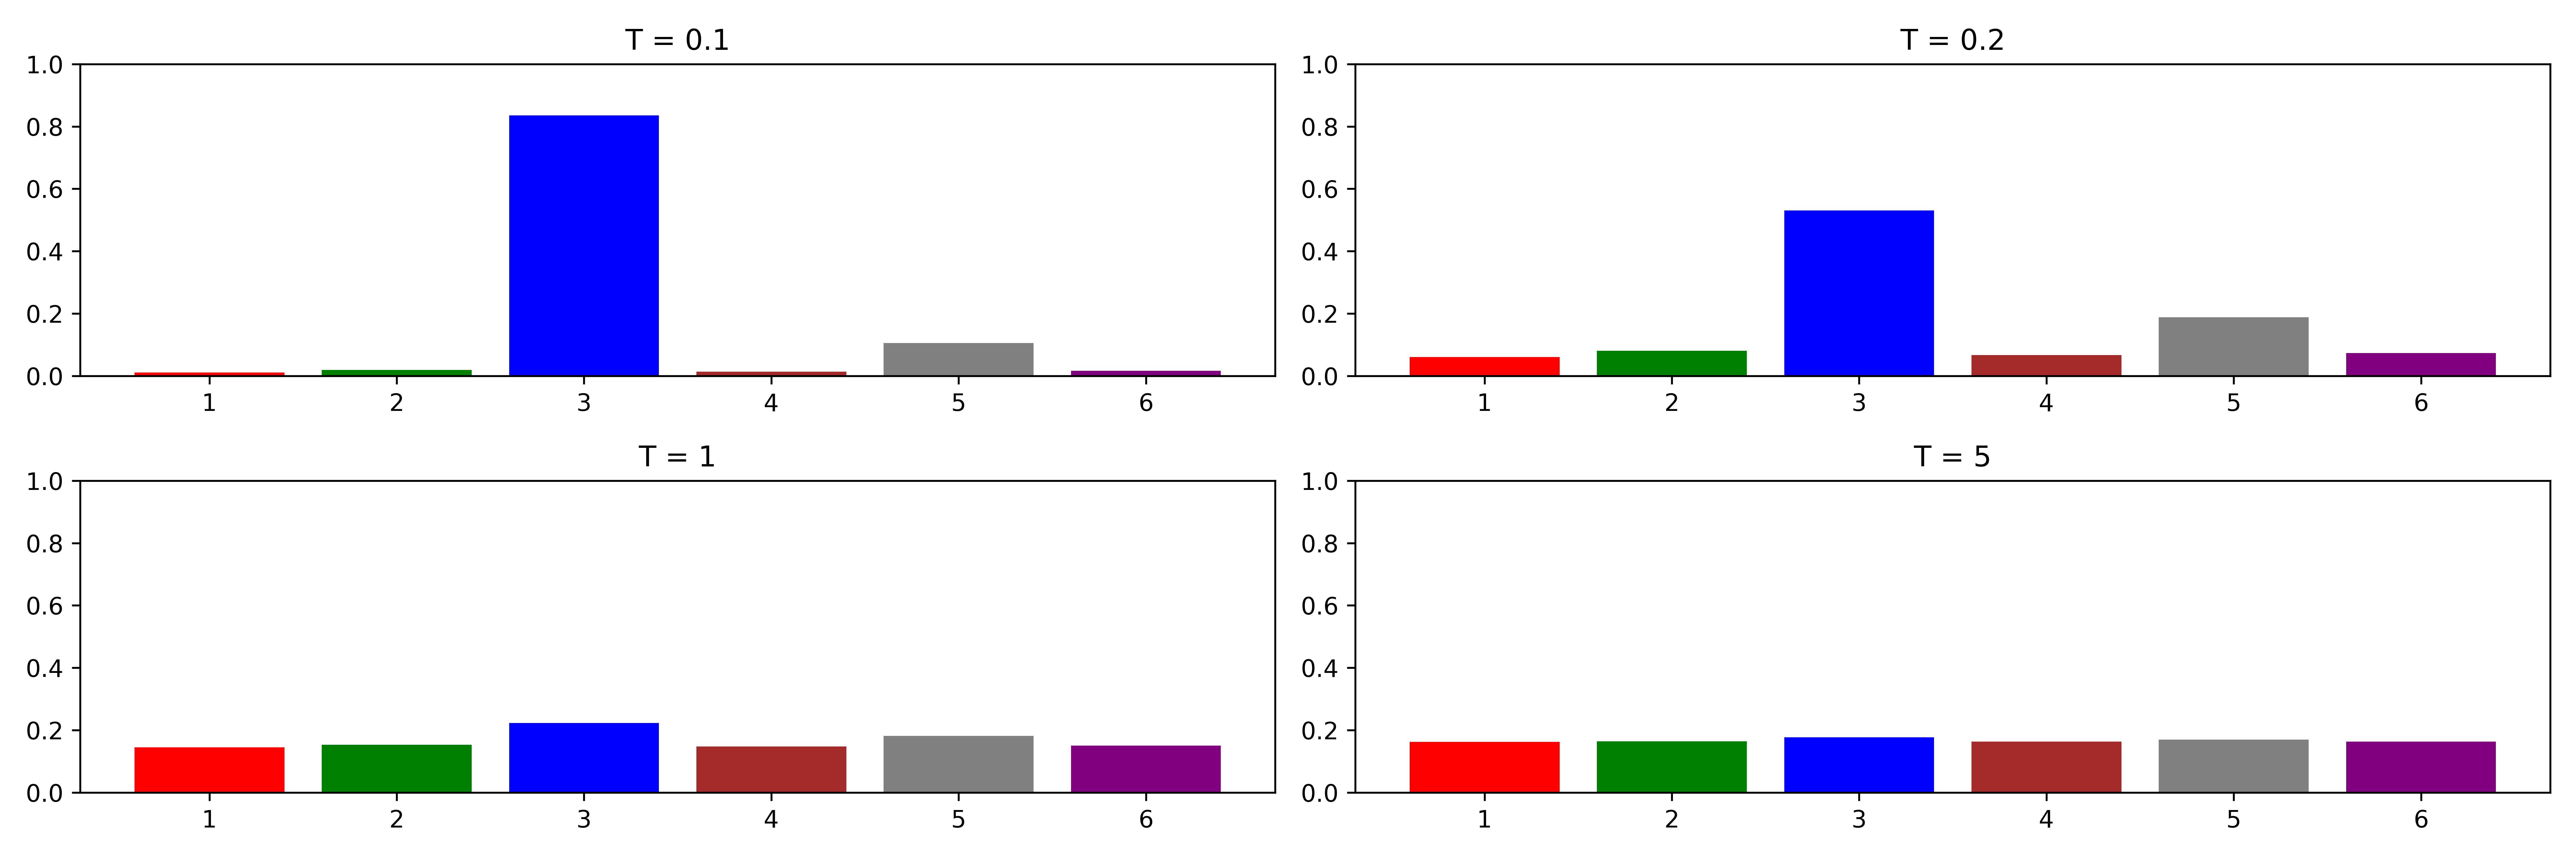
\includegraphics[scale=\myscale,scale=0.4]{figures/softmax-04}
\end{center}

Le vocable \og{}température\fg{} est issu de la physique statistique. Des particules dans un environnement proche du zéro absolu sont quasi-figées. Plus la température augmente plus elles atteignent des vitesses élevées.
Pour nous, le paramètre $T$ permet de prendre plus ou moins de liberté pour le choix du mot suivant. Avec une température très proche de $0$, on prend à coup sûr 
pour mot suivant celui le plus fréquent, avec une température élevée, on prend pour mot suivant un mot au hasard parmi les $k$ plus fréquents avec une probabilité $1/k$.

Voici des exemples de phrases commençant par \mot{the} obtenues pour différentes températures (le choix se fait à chaque fois parmi les 20 mots suivants les plus probables).
Pour $T=0.001$ c'est toujours la même successions de mots :
\mycenterline{\mot{
the company said it has been made by the company
}}

Voici trois phrases obtenues avec $T=0.05$ :
\mycenterline{\mot{
the company said the next week ended March 31	
}}
\mycenterline{\mot{
the company said it said it acquired by the second quarter		
}}
\mycenterline{\mot{
the end of the company said it will be held by the dollar		
}}


$T=0.5$ :
\mycenterline{\mot{
the dollar down slightly short notice about 18 pct this level	
}}
\mycenterline{\mot{
the world trade deficit and Trade Representative to help reduce debt		
}}



$T = 10$ :
\mycenterline{\mot{
the new business for delivery to an attempt was due for comment		
}}
\mycenterline{\mot{
the year earlier it expects oil reserves are in January 28		
}}



%--------------------------------------------------------------------
\subsection{Trigrammes}

On appelle \defi{bi-gramme} une suite (mot1, mot2) de deux mots consécutifs.
On appelle \defi{tri-gramme} une suite de $3$ mots consécutifs et plus généralement un $n$-gramme une suite de $n$ mots consécutifs.
La co-occurrence, c'est exactement compter les bi-grammes. Ce que nous avons fait précédemment, c'est utiliser ces valeurs pour choisir le mot2 qui doit suivre le mot1.
Améliorons notre méthode en comptant d'abord les tri-grammes, c'est-à-dire en comptant le nombre d'occurrences de tous les triplets (mot1, mot2, mot3).
Une fois ce travail effectué, étant donné une paire (mot1, mot2) on peut décider quels sont les mot3 les plus probables.

Voici des phrases commençant par \mot{the} puis \mot{company} et complétées par cette méthode (la température est $T=1$, le mot3 qui suit les deux mots précédents est choisi parmi les $20$ les plus probables) :
\mycenterline{\mot{
the company expects its overall retail income figures
}}
\mycenterline{\mot{
the company reported earnings from many countries to open the Japanese Government 
}}
\mycenterline{\mot{
the company with land holdings and production has become definitive
}}

Les phrases obtenues sont un peu plus naturelles que précédemment.
Nous avons compris une idée clé de la génération de texte par ordinateur : à partir d'un début de phrase, l'algorithme décide du mot suivant, puis recommence à partir de cette nouvelle liste de mots, jusqu'à obtenir une phrase complète.
Il s'agit maintenant d'améliorer la qualité des phrases obtenues.


%%%%%%%%%%%%%%%%%%%%%%%%%%%%%%%%%%%%%%%%%%%%%%%%%%%%%%%%%%%%%%%%%%%%%
\section{Tokens}

%--------------------------------------------------------------------
\subsection{Vocabulaire}

Commençons par établir la terminologie :
\begin{itemize}
	\item Le \defi{corpus} est l'ensemble des textes utilisés pour établir le modèle de prédiction. Ce corpus doit être le plus grand possible (plusieurs millions ou milliards de mots) mais aussi de bonne qualité puisque ce sont les statistiques issues de ces textes qui permettront de générer de nouvelles phrases.
	
	\item Les textes sont découpés en \defi{phrases} (que l'on peut définir en disant qu'elles commencent par une majuscule et finissent par un point).
	Les phrases sont composées de \defi{mots} (les mots sont séparés par des espaces). Chaque mot est formé de \defi{caractères} (par exemple, les lettres
	\mot{a}, \mot{b},\ldots, \mot{z} mais aussi les chiffres, la ponctuation).
\end{itemize}


Pour compléter un début de phrase, on va prédire une suite probable.
La prédiction se fait mot par mot. Nous allons à l'avenir utiliser un découpage différent en utilisant des \emph{tokens}.

Un \defi{token}\index{token} (une \defi{portion} ou un \defi{tronçon}) est une suite de caractères qui correspond à une partie de mot. Chaque modèle de langage fait son choix de tokens. L'ensemble des tokens choisis constitue le \defi{vocabulaire}.

Le modèle \emph{GPT2} utilise $50\,257$ tokens, chacun est numéroté. En voici quelques uns :

\begin{center}	
\begin{tabular}{ll}	
1009 & \mot{ution} \\
1010 & \mot{ters} \\
1011 & \mot{␣take} \\
1012 & \mot{␣Cl} \\
1013 & \mot{␣conf} \\
1014 & \mot{way} \\
\end{tabular} \qquad
\begin{tabular}{ll}	
1015 & \mot{ave} \\
1016 & \mot{␣going} \\
1017 & \mot{␣sl} \\
1018 & \mot{ug} \\
1019 & \mot{␣Americ} \\
\end{tabular}
\end{center}
	
Noter que dans ce modèle les majuscules et minuscules sont distinguées et que l'espace (ici notée par \mot{␣}) est prise en compte pour signifier que le token est un début de mot.
Par exemple \mot{Man}, \mot{man}, \mot{␣Man} et \mot{␣man} sont quatre tokens différents pour \emph{GPT2}.

%--------------------------------------------------------------------
\subsection{À quoi servent les tokens ?}


\begin{itemize}
	\item Les tokens servent à transformer une suite de mots en une liste de nombres.
	Par exemple la phrase :
	\mycenterline{\mot{mathematics is the queen of the sciences}}
	se transforme en la liste de tokens :
	\mycenterline{[\mot{mat}, \mot{hemat}, \mot{ics}, \mot{␣is}, \mot{␣the}, \mot{␣queen}, \mot{␣of}, \mot{␣the}, \mot{␣sciences}]}
	qui à son tour se transforme en une liste d'entiers (les \emph{tokens id}) :
	\mycenterline{[6759, 10024, 873, 318, 262, 16599, 286, 262, 19838]}
	
	Il s'agit d'un encodage sans perte d'information. À partir de la liste des tokens id, on retrouve les tokens et donc la phrase originale.
	
	\item Les tokens permettent de maîtriser la taille du vocabulaire.
	Par exemple le \emph{English Oxford Dictionnary} qui fait référence en langue anglaise, contient plus de $250\,000$ entrées. 
	Chaque mot fréquemment utilisé sera codé par un unique token, alors que les mots plus rares sont découpés en deux tokens ou plus. Il faut interpréter les tokens comme un intermédiaire entre un caractère et un mot complet :
	\mycenterline{caractère $\ \preccurlyeq\ $ token $\ \preccurlyeq\ $ mot}
	
	\item Les tokens peuvent faciliter un apprentissage logique des termes, par exemple en séparant la racine d'un mot et sa terminaison. Ce n'est cependant pas la motivation principale. Voici des exemples (fictifs) :
	\mycenterline{\mot{learning} = \mot{learn} + \mot{ing}}
	\mycenterline{\mot{surfing} = \mot{surf} + \mot{ing}}
	\mycenterline{\mot{learner} = \mot{learn} + \mot{er}}
    \mycenterline{\mot{surfer} = \mot{surf} + \mot{er}}	

	
\end{itemize}	
	
	
\emph{GPT2} a été entraîné sur un corpus d'environ 8 milliards de tokens (en anglais uniquement), \emph{GPT3.5} avec 500  milliards de tokens (dans plus de 100 langues différentes).


%--------------------------------------------------------------------
\subsection{Différents codages}

Nous allons résumer ici les différentes façons de coder un token parmi les $N$ tokens :
\begin{itemize}
	\item \defi{token} : une suite de caractères,
	\item \defi{l'identifiant token} (\emph{token id}) : l'entier $i$ avec $1 \le i \le N$ correspondant au rang du token dans la liste des tokens,
	\item \defi{vecteur identifiant token} (\emph{token id vector}) : le vecteur $e_i$ de la base canonique de $\Rr^N$ (où $i$ est l'identifiant du token).
\end{itemize}

Il ne faut pas confondre le vecteur identifiant $e_i$ avec son image $v_i  = \varphi(e_i) \in \Rr^n$ obtenue par plongement (voir plus loin). C'est ce vecteur image $v_i$ qui sera très important pour la suite, il sera appelé le \defi{vecteur token} (\emph{token vector/hidden state vector/embedding vector}).


\begin{exemple}
	
Dans le modèle \emph{GPT2} on a $N = 50\,257$ et $n=768$.

\myfigure{0.7}{
	\tikzinput{token-01}
} 

Pour le token \mot{␣cat}, dont l'identifiant est $3797$, le vecteur token débute par :
$v_{3797} = 
\left(\begin{smallmatrix}
0.0099 \\
0.0365 \\  
0.1640 \\
-0.2185 \\   
0.0285 \\
\vdots \\
\end{smallmatrix}\right).$
	
\end{exemple}

%--------------------------------------------------------------------
\subsection{Algorithme de tokenisation}

\textbf{Compression.}
La tokenisation a été inventée afin de compresser un texte sans perte d'information.
On considère qu'en moyenne un token regroupe $4$ caractères.
Et, également en moyenne, $4$ tokens forment $3$ mots.

\begin{exemple}
Si on considère un texte de 1000 caractères codés en ASCII, alors la taille mémoire nécessaire est $1000$ octets. La tokenisation transforme ce texte en une liste d'environ $250$ tokens, chaque token est codé sur $2$ octets (pour stocker son identifiant entre $0$ et $50\,257$). Ce qui donne une utilisation de $500$ octets, soit une compression de $50 \%$ sans perte d'information.
\end{exemple}

Pour nous, la tokenisation a pour principal but de fixer le nombre de mots du vocabulaire à une valeur souhaitée. Les mots rares ou inconnus sont alors découpés en plusieurs tokens.

\medskip

Expliquons l'algorithme BPE (\emph{Byte Pair Encoding})\index{token} qui permet d'obtenir une liste de tokens de taille voulue.
Les données initiales sont :
\begin{itemize}
	\item un texte (qui est le texte à compresser ou qui est le texte des données d'apprentissage),
	\item un vocabulaire initial qui est généralement la liste des caractères utilisés,
	\item un nombre $F$ de fusions (\emph{merge}) souhaitées.
\end{itemize}
L'algorithme renvoie le vocabulaire (la liste de tous les tokens) et le texte compressé (une liste de tokens).


\begin{algorithme}
\sauteligne
\begin{itemize}
	\item Transformer le texte en une liste de caractères.	
	\item Initialiser le vocabulaire à l'ensemble des caractères du texte.
	\item Répéter (au plus) $F$ fusions:
	\begin{itemize}
		\item Chercher la paire la plus fréquente de deux éléments du vocabulaire à des positions consécutives dans le texte.
		\item Ajouter cette paire fusionnée au vocabulaire et transformer le texte en utilisant cette fusion.
	\end{itemize}
	\item Renvoyer le vocabulaire et le texte.		
\end{itemize}
\end{algorithme}



\begin{exemple}
Considérons le texte : 
\mycenterline{\mot{ab ab abc dbac bacde}}
\begin{itemize}
	\item Ce texte est formé de $5$ mots, on représente chaque mot comme une liste de caractères.
	
\mycenterline{\ci{texte} = 
[\mot{a}, \mot{b}], [\mot{a}, \mot{b}], [\mot{a}, \mot{b}, \mot{c}],
[\mot{d}, \mot{b}, \mot{a}, \mot{c}],
[\mot{b}, \mot{a}, \mot{c}, \mot{d}, \mot{e}]
}

Le vocabulaire initial est formé des caractères :
\mycenterline{\ci{vocab} = [\mot{a}, \mot{b}, \mot{c}, \mot{d}, \mot{e}] }

\item \textbf{Fusion 1.}
On cherche dans les mots du texte les occurrences de paires de caractères.
La paire la plus fréquente est la paire (\mot{a}, \mot{b}) car \mot{ab} apparaît $3$ fois dans les mots (suivi de la paire \mot{ba} et de la paire \mot{ac} ayant chacune $2$ occurrences).
On ajoute \mot{ab} au vocabulaire et on ajuste le texte par fusion :

\mycenterline{\ci{vocab} = [\mot{a}, \mot{b}, \mot{c}, \mot{d}, \mot{e}, \mot{ab}] }

\mycenterline{\ci{texte} = 
	[\mot{ab}], [\mot{ab}], [\mot{ab}, \mot{c}],
	[\mot{d}, \mot{b}, \mot{a}, \mot{c}],
	[\mot{b}, \mot{a}, \mot{c}, \mot{d}, \mot{e}]
}

\item  \textbf{Fusion 2.}
On cherche dans les mots du texte les occurrences de paires de mots du nouveau vocabulaire. On fusionne ensuite \mot{b} et \mot{a} 
(2 occurrences de \mot{ba}) :

\mycenterline{\ci{vocab} = [\mot{a}, \mot{b}, \mot{c}, \mot{d}, \mot{e}, \mot{ab}, \mot{ba}] }

\mycenterline{\ci{texte} = 
[\mot{ab}], [\mot{ab}], [\mot{ab}, \mot{c}],
[\mot{d}, \mot{ba}, \mot{c}],
[\mot{ba}, \mot{c}, \mot{d}, \mot{e}]
} 

\item  \textbf{Fusion 3.}
La paire du vocabulaire la plus fréquente est maintenant la paire
(\mot{ba}, \mot{c}) avec $2$ occurrences. On les fusionne :

\mycenterline{\ci{vocab} = [\mot{a}, \mot{b}, \mot{c}, \mot{d}, \mot{e}, \mot{ab}, \mot{ba}, \mot{bac}] }

\mycenterline{\ci{texte} = 
	[\mot{ab}], [\mot{ab}], [\mot{ab}, \mot{c}],
[\mot{d}, \mot{bac}],
[\mot{bac}, \mot{d}, \mot{e}]
} 

\item Dans cet exemple, il n'y a plus de paires doublées, on s'arrête là.

\end{itemize}

Les tokens sont les éléments du vocabulaire que l'on numérote ici de $1$ à $8$.
Le texte tokenisé est alors codé sous la forme :
\mycenterline{\ci{texte} = [6], [6], [6,3], [4,8], [8,4,5]}

\end{exemple}

Pour \emph{GPT2} le vocabulaire initial est l'ensemble des $256$ caractères ASCII plus un caractère spécial (EOS, \emph{End Of Sentence}).
Le nombre de fusions est $F=50\,000$. L'algorithme va fournir un total de $50\,257$ tokens.
Il n'y a pas de raison de chercher à augmenter ce nombre de tokens. En effet, pour une langue donnée le nombre de mots utilisés est borné.




%%%%%%%%%%%%%%%%%%%%%%%%%%%%%%%%%%%%%%%%%%%%%%%%%%%%%%%%%%%%%%%%%%%%%
\section{Plongement}

Le but d'un plongement est de regrouper les mots par catégories.
Voici un exemple de regroupement que l'on peut obtenir pour les mots suivants :
\mycenterline{\mot{one}, \mot{two}, \mot{three}, \mot{four}, \mot{five}, \mot{six}, \mot{seven}, \mot{eight}, \mot{nine}, \mot{ten}}

\mycenterline{\mot{doctor}, \mot{lawyer}, \mot{teacher}, \mot{engineer}, \mot{scientist}, \mot{artist}, \mot{writer}, \mot{actor}, \mot{singer}, \mot{dancer}}

\mycenterline{\mot{red}, \mot{green}, \mot{blue}, \mot{yellow}, \mot{orange}, \mot{purple}, \mot{pink}, \mot{brown}, \mot{black}, \mot{white}}

\begin{center}
	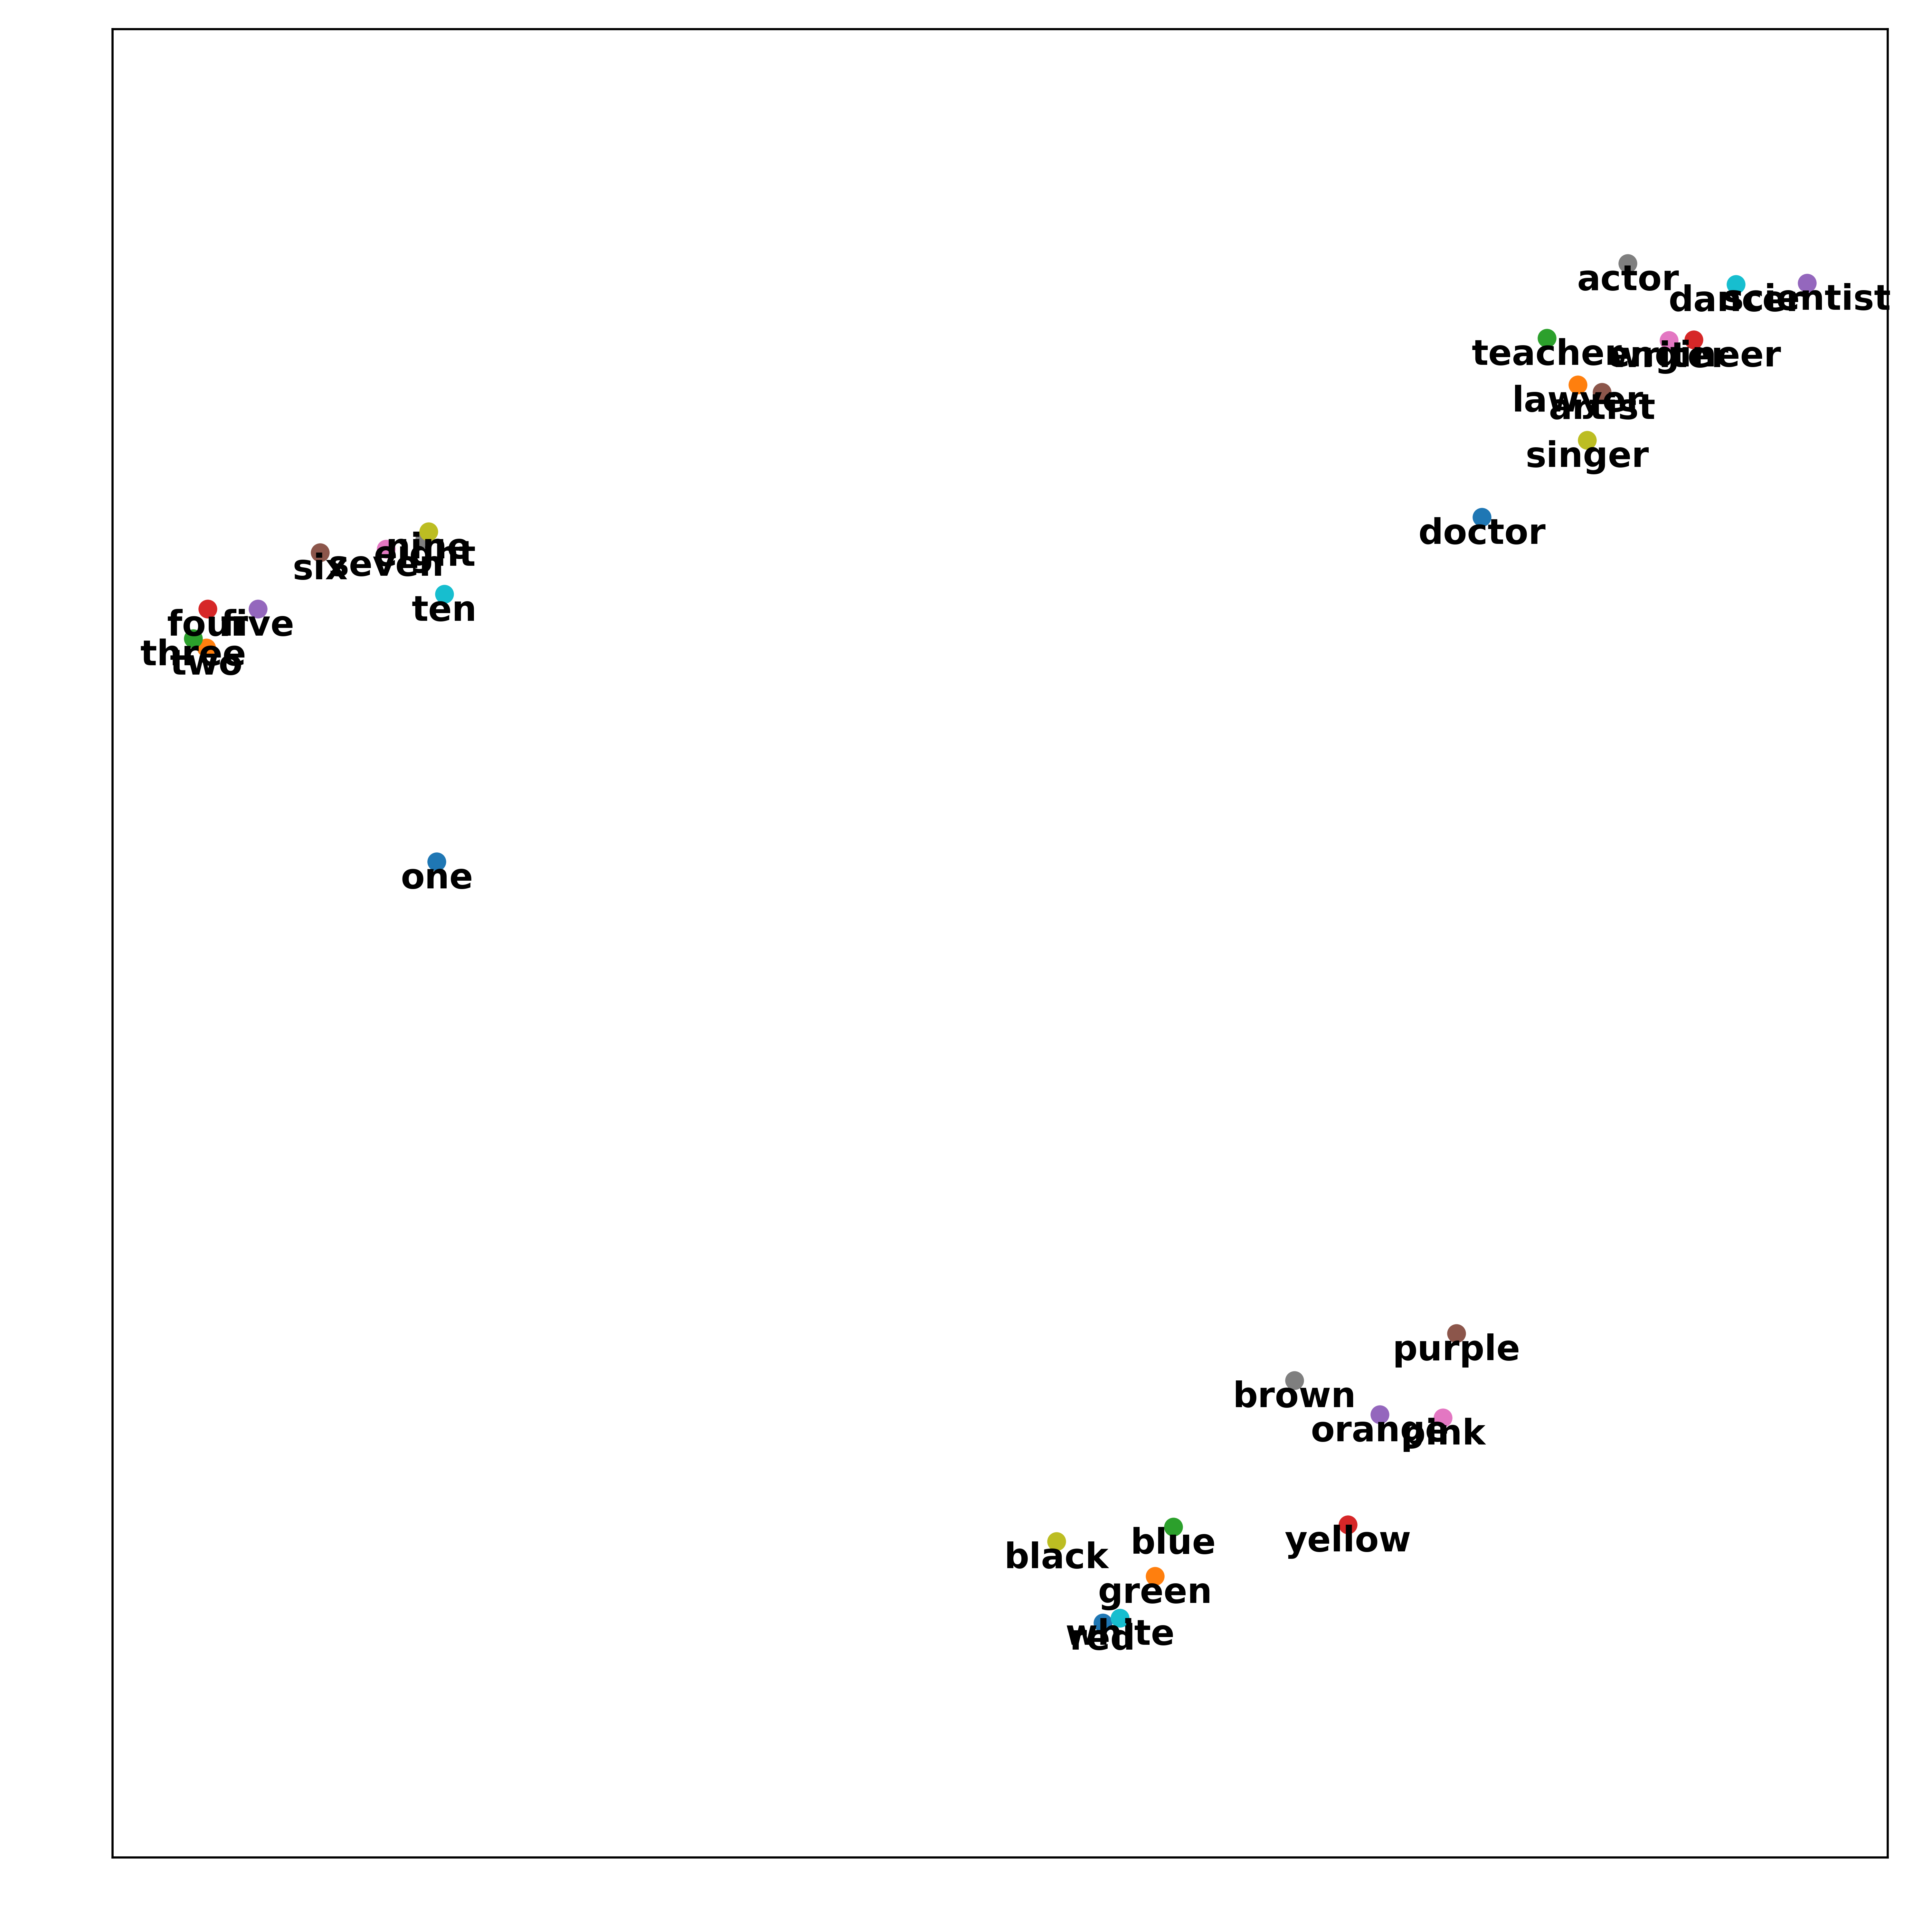
\includegraphics[scale=\myscale,scale=0.3]{figures/projection-pca-0.png}
\end{center}

On note bien le regroupement par catégories : les chiffres, les professions et les couleurs.
Cependant cette représentation dans le plan ne donne qu'une idée partielle du résultat car chaque mot sera en fait représenté par un point (plus exactement par un vecteur) dans un espace de grande dimension.



%--------------------------------------------------------------------
\subsection{Un mot est un vecteur}

\textbf{Plongement.}\index{plongement}
Nous allons transformer un mot (ou plus exactement un token) en un vecteur.
Cette opération s'appelle le plongement.
Mathématiquement cela correspond à une fonction (une application linéaire) :
$$
\begin{array}{rccc}
	\varphi : & \Rr^N & \longrightarrow & \Rr^n \\
	          & e_i   & \longmapsto     & v_i  
\end{array}
$$

\begin{itemize}
	\item $N$ est le nombre total de tokens (par exemple $N=50\,257$ pour \emph{GPT2} et environ $100\,000$ pour \emph{GPT3.5} et \emph{GPT4}),
	
	\item $n$ est la \defi{dimension de plongement}, par exemple $n=768$ pour \emph{GPT2} (et entre $1024$ et $2048$ pour les modèles plus récents).
	
	\item $e_i$ est le vecteur identifiant le token numéro $i$ (avec $1 \le i \le N$), c'est le $i$-ème vecteur de la base canonique de $\Rr^N$.
	
	\item $v_i = \varphi(e_i)$ est le \defi{vecteur token}.
\end{itemize}


Une fois les tokens définis (voir la section précédente) ce plongement est calculé une fois pour toutes.



\medskip

\textbf{Matrice.} Comme $\varphi$ est une application linéaire, elle est définie par une matrice $A \in M_{n,N}$ ayant $n$ lignes et $N$ colonnes.
La $i$-ème colonne de la matrice $A$ est le vecteur $v_i$. Cette matrice s'appelle la \defi{matrice de plongement}.
Ainsi, en termes de vecteurs, nous avons simplement :
$$v_i =  A e_i.$$


Remarques mathématiques :
$\varphi$ est une application linéaire. Comme on a défini $\varphi$ sur la base canonique de $\Rr^N$, $\varphi$ s'étend par linéarité sur tout $\Rr^N$, mais nous n'en aurons pas vraiment besoin. D'autre part, le mot plongement n'est pas ici un plongement au sens mathématique usuel.

\medskip

\textbf{Point ou vecteur ?} 
On peut à la fois considérer $v_i$ comme un point ou bien comme un vecteur de $\Rr^n$.
Si on considère les éléments de $\Rr^n$ comme des points, alors 
la distance entre deux points $X$ et $Y$ est par exemple la \defi{distance euclidienne} définie par :
$$\| X-Y \| = \sqrt{\sum_{i=1}^n (x_i - y_i)^2}.$$

\myfigure{0.8}{
	\tikzinput{cosinus-02}
} 

Mais en fait nous allons considérer les éléments de $\Rr^n$ comme des vecteurs.
La \defi{similarité cosinus}\index{similarite@similarité cosinus} entre $X$ et $Y$ est le cosinus de l'angle entre ces deux vecteurs :
$$S_{\cos}(X,Y) = \cos(\theta) = \frac{\langle X \mid Y \rangle}{\| X \| \; \| Y\| }.$$
On a $\cos (\theta) \in [-1,1]$, ce n'est pas une distance au sens mathématique usuel.

Cette formule provient d'une formule qui relie le produit scalaire à l'angle entre deux vecteurs :
$$\langle X \mid Y \rangle  = \| X \| \ \| Y \| \cos(\theta)$$
où on rappelle que :
\begin{itemize}
	\item $\langle X \mid Y \rangle  = x_1y_1+x_2y_2+\cdots +x_ny_n$ est le produit scalaire des vecteurs $X$ et $Y$,
	\item $\| X \| = \sqrt{x_1^2+\cdots+x_n^2}$ et $\| Y \| = \sqrt{y_1^2+\cdots+y_n^2}$ sont les normes de $X$ et $Y$,
	\item $\theta$ est l'angle entre les vecteurs $X$ et $Y$.
\end{itemize}

\begin{itemize}
	\item Plus $\cos(\theta)$ est proche de $1$, plus l'angle est proche de $0$ et alors  les vecteurs ont presque la même direction et le même sens,
	\item plus $\cos(\theta)$ est proche de $-1$, plus l'angle est proche de $\pi$ et alors les vecteurs ont presque la même direction mais des sens contraires,
	\item si $\cos(\theta)$ est proche de $0$ alors les vecteurs sont presque orthogonaux.
\end{itemize}

\myfigure{0.7}{
	\tikzinput{cosinus-03}
} 


\begin{exemple}
Soient $X = \left(\begin{smallmatrix}2 \\ 3 \end{smallmatrix}\right) \in \Rr^2$ et $Y = \left(\begin{smallmatrix}4 \\ 4 \end{smallmatrix}\right)\in \Rr^2$.

\myfigure{0.9}{
	\tikzinput{cosinus-01}
} 

\begin{itemize}
	\item Distance euclidienne $\|X-Y\| = \sqrt{(2-4)^2 + (3-4)^2} = \sqrt5 \simeq 2.24$.
	 
	\item Similarité cosinus : $S_{\cos}(X,Y) = \frac{2\cdot 4 + 3\cdot4}{\sqrt{13}\sqrt{32}} = \frac{5}{\sqrt{26}} \simeq 0.98$. Le cosinus est proche de $1$ donc l'angle $\theta$ est proche de $0$.
\end{itemize}	
\end{exemple}

\begin{exemple}
Dans le modèle \emph{GPT2} les tokens \mot{␣dog} et \mot{␣cat} ont pour vecteurs plongés :

$$v_{\text{\mot{␣dog}}} = \begin{pmatrix}
	 0.0944 \\
	 -0.0771 \\
	 0.0346 \\
	 -0.0351 \\
	 -0.0892 \\ 
     \vdots \\
     \end{pmatrix} \in \Rr^{768}
\qquad \qquad
v_{\mot{␣cat}} = \begin{pmatrix}
	0.0099 \\
	0.0365 \\
	0.1640 \\
	-0.218 \\
	0.0285 \\
	\vdots
\end{pmatrix} \in \Rr^{768}
$$
\begin{itemize}
	\item La similarité cosinus 
$S_{\cos} (v_{\text{\mot{␣dog}}}, v_{\text{\mot{␣cat}}} ) \simeq 0.55$
soit un angle $\theta \simeq 57^\circ$. Ainsi le mots \mot{␣dog} et \mot{␣cat} sont bien distingués.
    \item Le token le plus proche de \mot{␣dog} est \mot{␣dogs} (au pluriel) avec une similarité de $0.79$ (soit $\theta \simeq 38^\circ$). Parmi les $50\,257$ tokens, les plus similaires à \mot{␣dog} sont dans l'ordre :
\mycenterline{ \mot{␣dogs}, \quad \mot{␣Dog}, \quad \mot{Dog}, \quad \mot{canine}, \quad \mot{dog}, \quad
	\mot{␣Dogs}, \quad \mot{␣puppy}, \quad \mot{␣pet}, \quad \mot{␣cat}, \quad\ldots
}
    \item Le token le moins similaire est \mot{␣Stephenson} avec une similarité de $0.08$ (soit $\theta \simeq 85^\circ$).
\end{itemize} 
\end{exemple}

On retient que si la similarité cosinus est proche de $1$, les mots ont des significations proches. Selon les modèles, une similarité cosinus proche de $-1$ peut indiquer que les mots ont des significations opposées et si la similarité cosinus est proche de $0$ les mots n'ont pas de lien entre eux.

\smallskip

Remarque importante : la similarité cosinus $S_{\cos}(X,Y)$ ne dépend que de la direction de $X$ et de $Y$, pas de la longueur des vecteurs.


% Remarque : dans certains modèles linguistiques, les coordonnées des vecteurs tokens $f_i$ sont toutes positives, c'est-à-dire $v_i \in (\Rr_+)^n$. 
% 	Dans ce cas le produit scalaire de deux tels vecteurs est positif ou nul et on aurait $\cos(\theta) \in [0,1]$.

\begin{exemple}
Dans notre situation linguistique, la longueur du vecteur correspond à la certitude que l'on a dans notre résultat.

\myfigure{0.9}{
	\tikzinput{cosinus-04}
} 

\end{exemple}

\medskip

\textbf{Pourquoi utiliser la similarité cosinus ?}
Voici une explication sous la forme d'un exemple (fictif).
\begin{exemple}
Chacun de nos axes de $\Rr^n$ correspond à une catégorie, par exemple un axe pour \mot{homme}, un axe pour \mot{femme}, un axe pour \mot{enfant}, un axe pour \mot{royauté}\ldots{} (évidemment dans la réalité ce ne sera pas aussi simple).
Dans ces coordonnées (\mot{homme}, \mot{femme}, \mot{enfant}, \mot{royauté}) de $\Rr^4$ imaginons que le mot \mot{roi} ait pour direction le vecteur 
$X_1 = \left(\begin{smallmatrix}1\\0\\0\\1\end{smallmatrix}\right)$ 
(c'est autant un homme qu'un symbole de royauté),
la mot \mot{reine} a pour direction le vecteur 
$X_2 = \left(\begin{smallmatrix}0\\1\\0\\1\end{smallmatrix}\right)$
 et \mot{princesse} 
 $X_3 = \left(\begin{smallmatrix}0\\1\\1\\1\end{smallmatrix}\right)$.


\begin{center}
	\begin{tabular}{lccc}
					 & \mot{roi} & \mot{reine} & \mot{princesse}  \\
	\mot{homme}      & 1 & 0 & 0 \\
	\mot{femme}      & 0 & 1 & 1 \\
	\mot{enfant}	 & 0 & 0 & 1 \\
	\mot{royaute}	 & 1 & 1 & 1 \\
	\end{tabular}
\end{center}

Si dans une phrase on trouve trois fois le mot \mot{homme} et aussi le mot \mot{couronne} et le mot \mot{château} (deux symboles de royauté), on va associer à ce texte le vecteur $Y = \left(\begin{smallmatrix}3\\0\\0\\2\end{smallmatrix}\right)$ obtenu en comptant les occurrences de chaque catégorie.

Calculons la similarité cosinus entre $Y$ et les $X_i$ :
$$
S_{\cos}(X_1,Y) \simeq 0.98 \qquad
S_{\cos}(X_2,Y) \simeq 0.39 \qquad
S_{\cos}(X_3,Y) \simeq 0.32 
$$

La similarité cosinus entre $Y$ et $X_1$ (\mot{roi}) est plus forte que celle entre $Y$ et $X_2$ (\mot{reine}) et entre $Y$ et  $X_3$ (\mot{princesse}). Il est donc naturel d'associer à notre phrase le mot \mot{roi}.


Noter qu'en terme de distance euclidienne $X_1$ (pour \mot{roi}) et $Y$ (pour notre phrase) sont éloignés.
\end{exemple}


\begin{exemple}
Poursuivons cet exemple. Cette fois, notre tâche est de résumer un texte par un seul mot.
On procède de la façon suivante : chaque fois qu'on rencontre le terme \mot{roi}, on ajoute le vecteur
$X_1 = \left(\begin{smallmatrix}1\\0\\0\\1\end{smallmatrix}\right)$,
chaque fois qu'on rencontre le mot \mot{princesse}, on ajoute le vecteur
$X_3 = \left(\begin{smallmatrix}0\\1\\1\\1\end{smallmatrix}\right)$, etc.
Un long conte rempli de princesses nous donnera un vecteur de grande norme, tandis qu’un court texte sur le même sujet produira un vecteur de norme plus petite.
Cependant, si notre processus est bien calibré, ces deux vecteurs devraient avoir (à peu près) la même direction.
\end{exemple}


\medskip

\textbf{La malédiction de la dimension.}  

Nos sens ne sont pas adaptés aux espaces de grande dimension. Si l’on prend au hasard $1000$ points dans $\Rr^{768}$, avec des coordonnées tirées uniformément dans $[0,1]$, alors la distance entre deux points quelconques sera en moyenne d’environ $11.3$, avec un écart-type de seulement $0.25$.  
Cela signifie que presque tous les points sont situés à une distance comprise entre $11.0$ et $11.5$ les uns des autres. Il n’y a donc plus vraiment de distinction entre points proches et points éloignés. La distance euclidienne n'est donc plus pertinente.

Dans notre contexte, les vecteurs représentant les textes ou les mots sont souvent \emph{très creux} : la grande majorité de leurs composantes sont nulles (ou négligeables). Par exemple, un vecteur peut n’avoir que $50$ composantes non nulles sur $768$ (bien sûr ce ne sont pas toujours les mêmes composantes nulles à chaque fois). La distance euclidienne ne permet pas de profiter de ce fait.

En revanche, la similarité cosinus compare essentiellement la direction des vecteurs en ignorant implicitement les coordonnées nulles. Elle permet donc de calculer comme si on était dans l'espace des composantes non-nulles, donc de se ramener à des calculs en dimension $50$ au lieu de $768$ pour notre exemple. Ainsi la similarité cosinus permet de mieux distinguer des mots proches de mots éloignés.





%--------------------------------------------------------------------
\subsection{Projections}

\index{projection}

\textbf{Projections.}
Les mots/tokens vont être plongés dans un espace $\Rr^n$ de grande dimension, par exemple avec $n=768$ ou $n=1024$. 
Notre perception est limitée aux dimensions $2$ (le plan) et $3$ (l'espace), on va donc se ramener à cette situation pour nos illustrations graphiques.

On se représente bien un carré (à gauche) et aussi un cube de l'espace projeté sur un plan (au centre), mais il est plus difficile de bien visualiser un hyper-cube de $\Rr^4$ (à droite avec les coordonnées de chaque sommet).


\begin{center}
\begin{minipage}{0.25\textwidth}
\myfigure{0.8}{
	\tikzinput{cube-01}
 } 	
\end{minipage}
\begin{minipage}{0.3\textwidth}
\myfigure{0.8}{	
 	\tikzinput{cube-02}
 } 
\end{minipage}	
\begin{minipage}{0.4\textwidth}
\myfigure{0.8}{ 	
 	\tikzinput{cube-03}
 } 
\end{minipage} 
\end{center}

Nous allons projeter les éléments de $\Rr^n$ dans le plan ou l'espace.
Nous notons $\pi$ cette projection :
$$\pi : \Rr^n \to \Rr^2 \qquad \text{ ou } \qquad \pi : \Rr^n \to \Rr^3$$



%Une telle projection 
%$\pi : \Rr^2 \to \Rr$ est défini par une matrice $P \in M_{2,n}$ (à $2$ lignes et $n$colonnes) vérifiant $P^2=P$, c'est-à-dire $\pi(X) = PX$. 
%Pour $\pi : \Rr^3 \to \Rr$ on a $\pi(X)= PX$ avec  $P \in M_{3,n}$ avec $P^2=P$.

\bigskip

\textbf{Projections sur une droite.}
Voici la formule pour projeter orthogonalement un vecteur $x \in \Rr^n$ sur une droite dirigée par un vecteur $u \in \Rr^n$ de norme $1$ :
$$p(x) = \langle x \mid u \rangle u$$
On obtient une fonction à valeurs réelles en ne retenant que le produit scalaire : $\pi : \Rr^n \to \Rr$ définie par $\pi(x) = \langle x \mid u \rangle$.

\myfigure{1}{ 	
	\tikzinput{projection-01}
} 

On peut bien sûr définir le vecteur $u$ à la main, mais on peut aussi choisir pour $u$ un vecteur calculé par le plongement comme dans l'exemple suivant.
Nous allons utiliser le modèle \emph{BERT} qui a pour avantage d'avoir beaucoup de mots entiers qui sont des tokens, ce qui rend les exemples plus compréhensibles. \emph{BERT} compte $30\,522$ tokens, parmi ceux-ci plus de $20\,000$ sont des mots complets. Le plongement de \emph{BERT} associe à chaque token un vecteur de $\Rr^{768}$.

\begin{exemple}
Considérons des noms d'animaux et des noms de villes :
\mycenterline{
\mot{cat}, \mot{dog}, \mot{mouse}, \mot{elephant}, \mot{lion}, \mot{tiger}, \mot{bear}, \mot{wolf}, \mot{horse}, \mot{zebra}
}
\mycenterline{
\mot{paris}, \mot{berlin}, \mot{madrid}, \mot{rome}, \mot{lisbon}, \mot{brussels}, \mot{amsterdam}, \mot{vienna}, \mot{athens}
}

On souhaite visualiser si le plongement du modèle (ici \emph{BERT}) distingue bien ces mots.
On pourrait définir à la main un vecteur $u \in \Rr^{768}$ et projeter chaque vecteur $v_i$ sur la droite dirigée par $u$, mais il n'est pas facile de faire un choix judicieux pour $u$.

Il est plus malin de calculer d'abord les plongements $v_{\text{\mot{animal}}}$ et 
$v_{\text{\mot{city}}}$ des tokens \mot{animal} et \mot{city}. Puis on définit pour $u$ le vecteur :
	$$u = v_{\text{\mot{animal}}} - v_{\text{\mot{city}}}$$
(que l'on peut rendre unitaire si besoin).
Ensuite on considère la projection sur la droite dirigée par $u$ :
pour chaque vecteur token $v_i$ on calcule le produit scalaire $\langle v_i \mid u \rangle$. Si notre modèle est correct alors plus ce produit scalaire est haut, plus le token correspond à la catégorie \og{}animaux\fg{}, plus le produit scalaire est bas, plus le token correspond à la catégorie \og{}villes\fg{}.

Voici le tracé de nos mots obtenus par cette méthode :

\begin{center}
	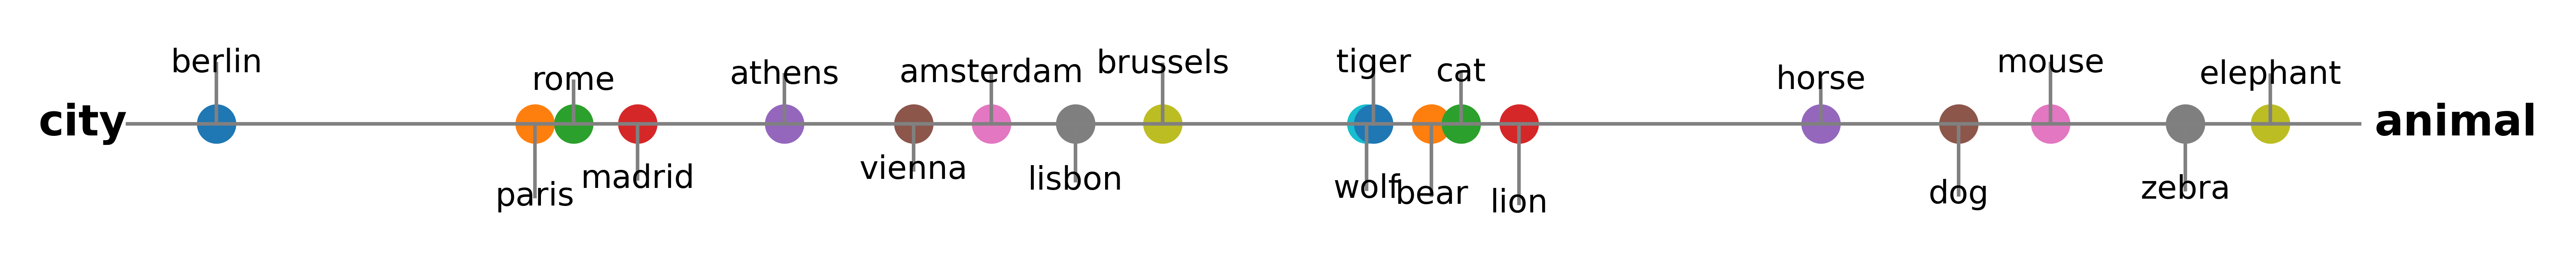
\includegraphics[scale=\myscale,scale=0.63]{figures/projection-droite}
\end{center}

On constate que le modèle sépare correctement les villes (à gauche) des animaux (à droite).
\end{exemple}


\bigskip

\textbf{Projection sur un plan ou sur un espace.}
La formule précédente s'étend naturellement en dimension $2$ et $3$.
Considérons les vecteurs $u,v \in \Rr^n$ formant une base orthonormée (c'est-à-dire $\|u\| = 1$, $\|v\| = 1$ et $\langle u \mid v \rangle =0$), la projection orthogonale sur le plan défini par $(u,v)$ est l'application $\pi : \Rr^n \to \Rr^2$ définie par 
$$\pi(x) = \big(\langle x \mid u \rangle, \langle x \mid v \rangle\big).$$

\myfigure{1}{ 	
	\tikzinput{projection-02}
} 


De même pour $u,v,w \in \Rr^n$ formant une base orthonormée, $\pi : \Rr^n \to \Rr^3$ est définie par 
$$\pi(x) = \big(\langle x \mid u \rangle, \langle x \mid v \rangle, \langle x \mid w \rangle\big).$$

\begin{exemple}
Voici la projection d'une liste de tokens de fruits et de pays sur le plan de $\Rr^{768}$ engendré par les vecteurs $u = f_1 = \left(\begin{smallmatrix}1 \\ 0 \\ 0 \\ 0 \\ \vdots \end{smallmatrix}\right)$ et $v = f_3 =  \left(\begin{smallmatrix}0 \\ 0 \\ 1 \\ 0 \\\vdots \end{smallmatrix}\right)$.


\begin{center}
	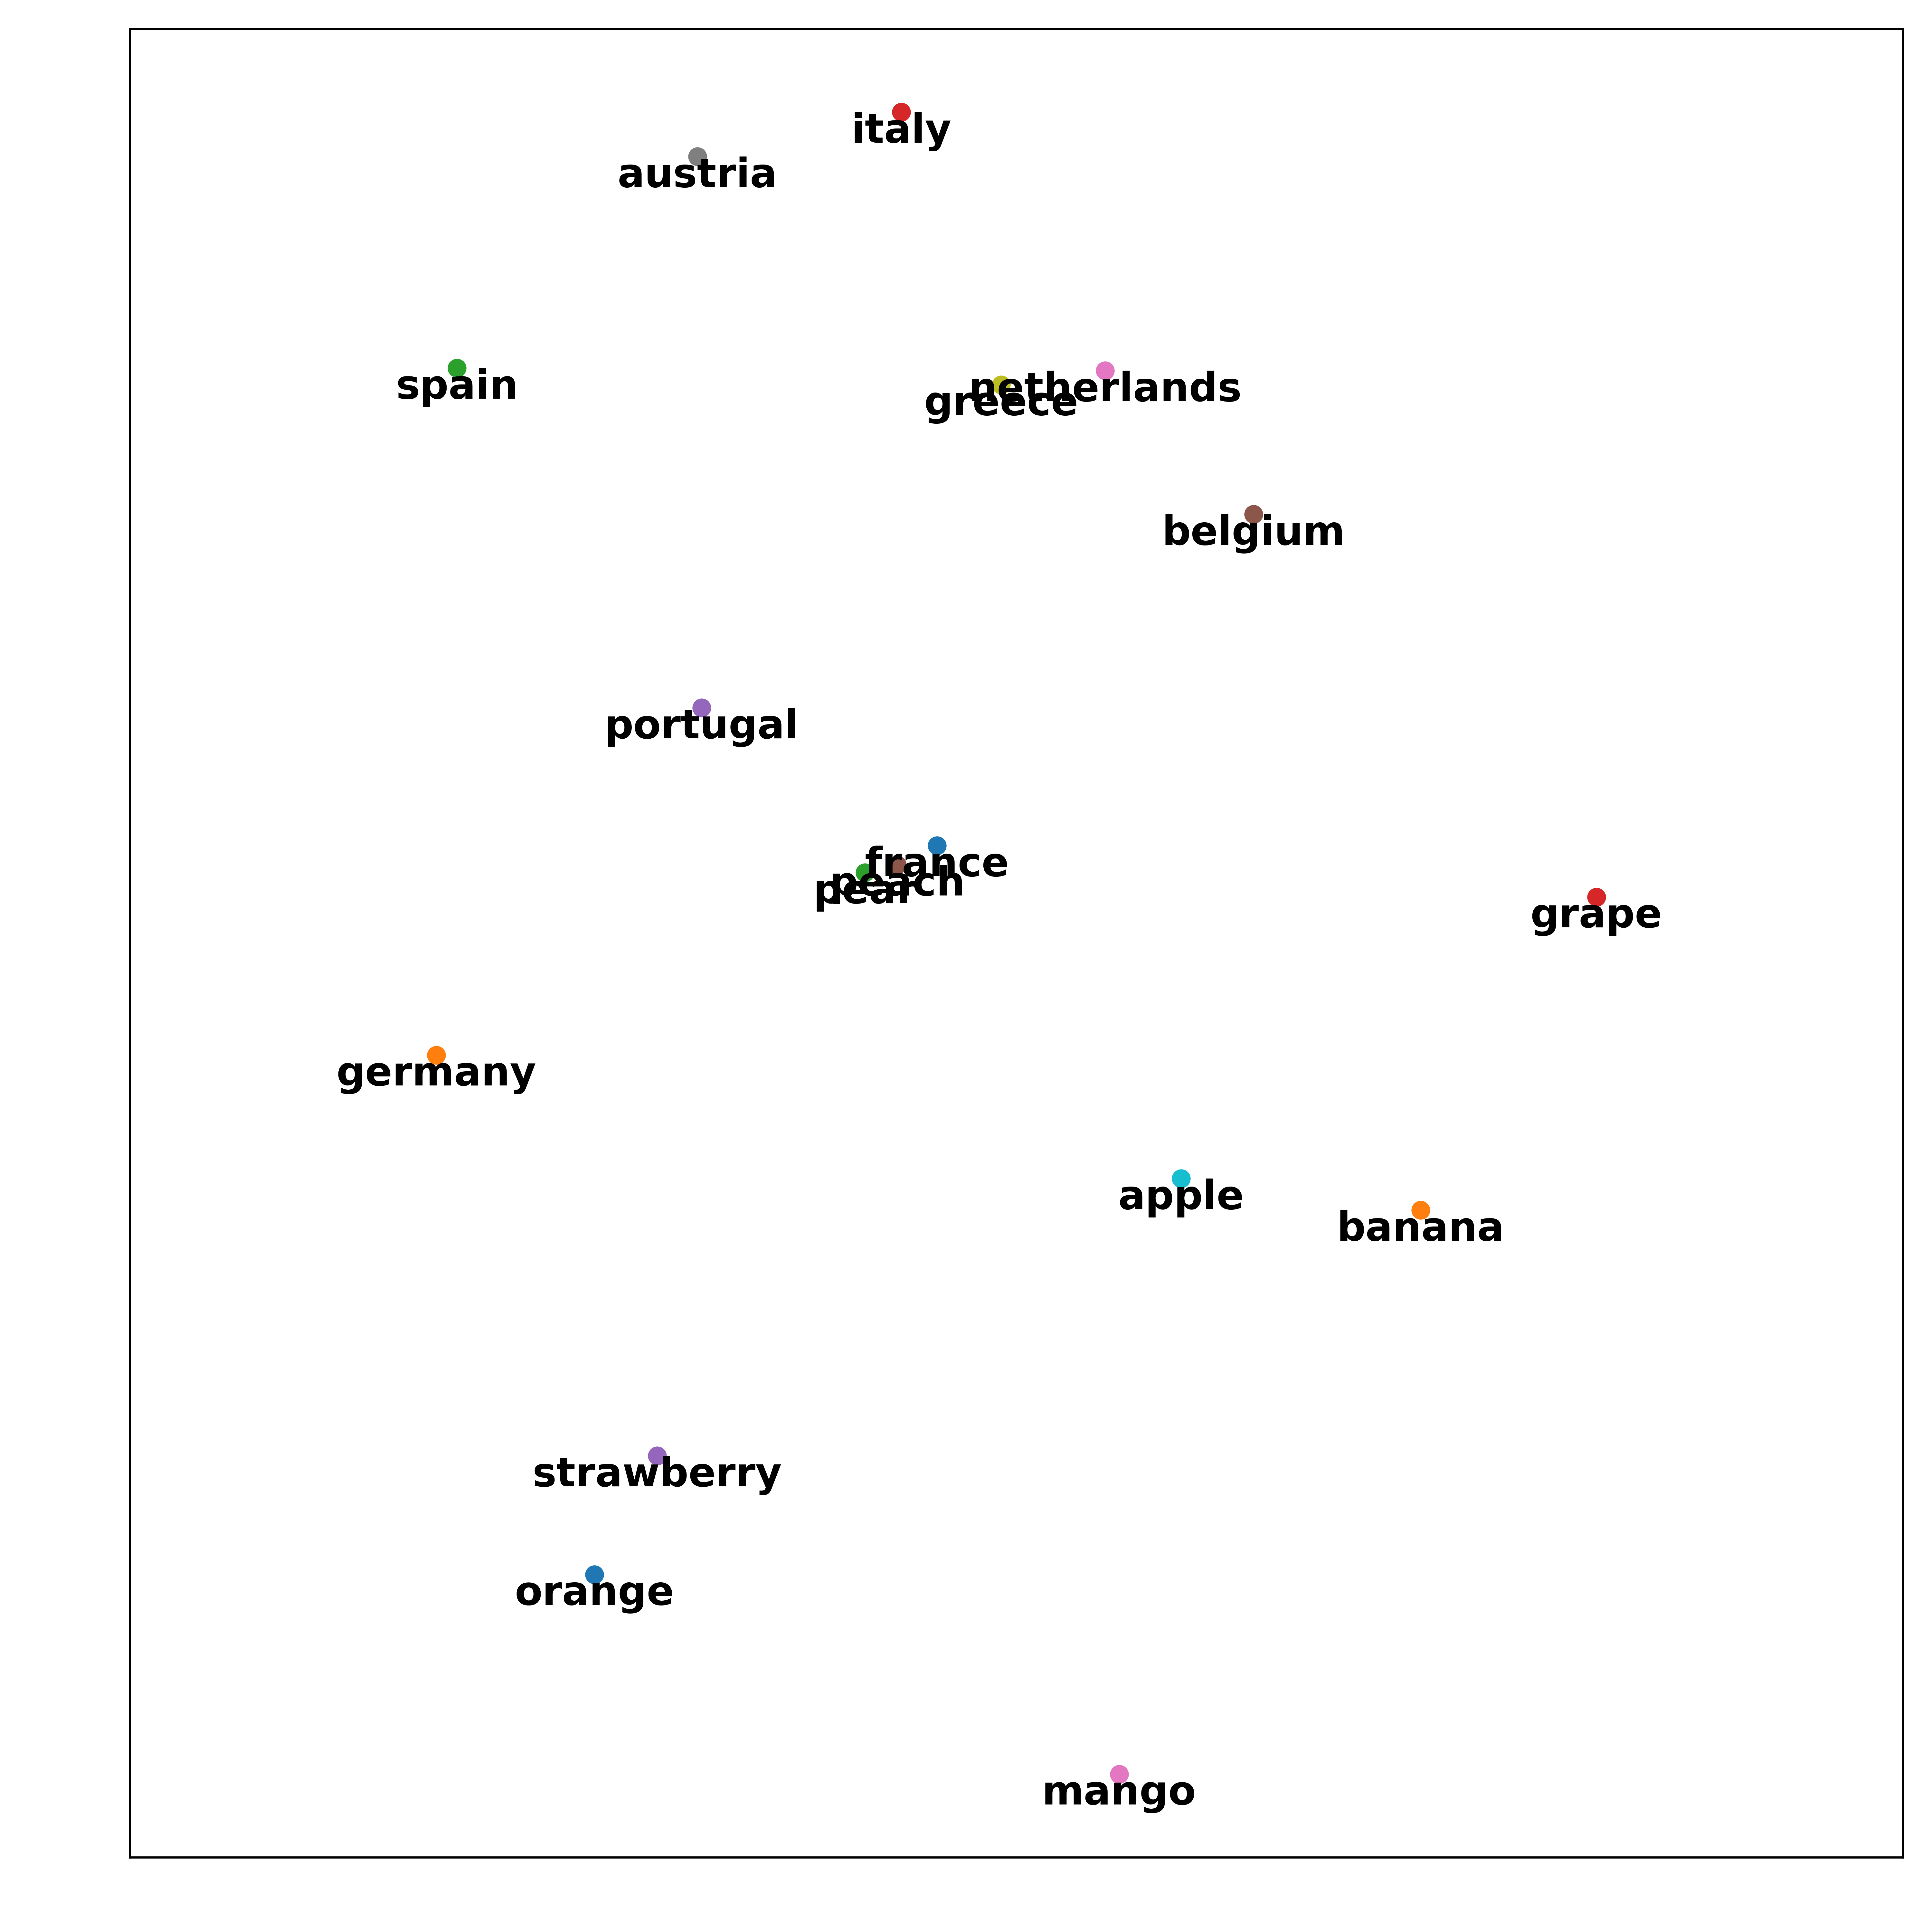
\includegraphics[scale=\myscale,scale=0.3]{figures/projection-plan}
\end{center}

Noter que globalement la séparation entre les fruits et les pays est correcte, sauf pour les tokens \mot{pear}, \mot{peach}, \mot{france} regroupés au centre.
Cela ne signifie pas que le modèle sépare mal ces tokens, mais juste que notre projection ne montre pas correctement cette séparation.
\end{exemple}

Revenons sur le dernier point soulevé par cet exemple avec deux analogies.
Lorsque vous observez le ciel étoilé, ce n'est pas parce que deux étoiles vous semblent proches dans le ciel, qu'elles le sont réellement. L'une peut être beaucoup plus éloignée de la Terre que l'autre. 
Une autre analogie est la suivante : lorsque vous regardez une radio d'un corps humain il est difficile de reconstituer la situation 3D, c'est d'ailleurs pour cela que l'on fait souvent des radios suivant plusieurs points de vue. 
Ici, il est illusoire de vouloir comprendre un espace de dimension $768$ ou plus en n'étudiant seulement que quelques projections.
Cependant nous allons voir comment obtenir des projections plus pertinentes que d'autres.


\bigskip


\textbf{Analyse en composantes principales.}
Comment trouver une bonne projection qui mette le mieux en évidence l'étalement de nos données ? Il existe une technique statistique appelée analyse en composantes principales (\emph{pca}, \emph{principal component analysis}). 
Nous ne cherchons pas à expliquer cette méthode un peu sophistiquée, mais qui s'écrit en quelques lignes en \Python{}. Ici \ci{X} est une liste \ci{numpy} de vecteurs de $\Rr^n$, et cette fonction renvoie la projection de ces vecteurs dans le plan ($k=2$) ou l'espace ($k=3$).

\begin{center}
\begin{lstlisting}
def pca(X, k=2):
	Xmean = X.mean(axis=0)                                  # Moyenne
	XX = X - Xmean                              # Centrer les données	
	C = np.dot(XX.T, XX) / (XX.shape[0] - 1)  # Matrice de covariance	
	d, u = np.linalg.eigh(C)       # Décomposition en valeurs propres	
	idx = np.argsort(d)[::-1]               # Tri des valeurs propres	
	u = u[:, idx]                          # Tri des vecteurs propres	
	U = u[:, :k]     # Projection sur les k premiers vecteurs propres
	return np.dot(XX, U)
\end{lstlisting}
\end{center}

\begin{exemple}
En reprenant l'exemple précédent avec la projection obtenue par notre nouvelle méthode, on constate que cette fois les fruits sont clairement séparés des pays (ci-dessous à gauche). Sur la figure de droite on a projeté tous les $30\,522$ tokens de \emph{BERT}. 
\begin{center}
	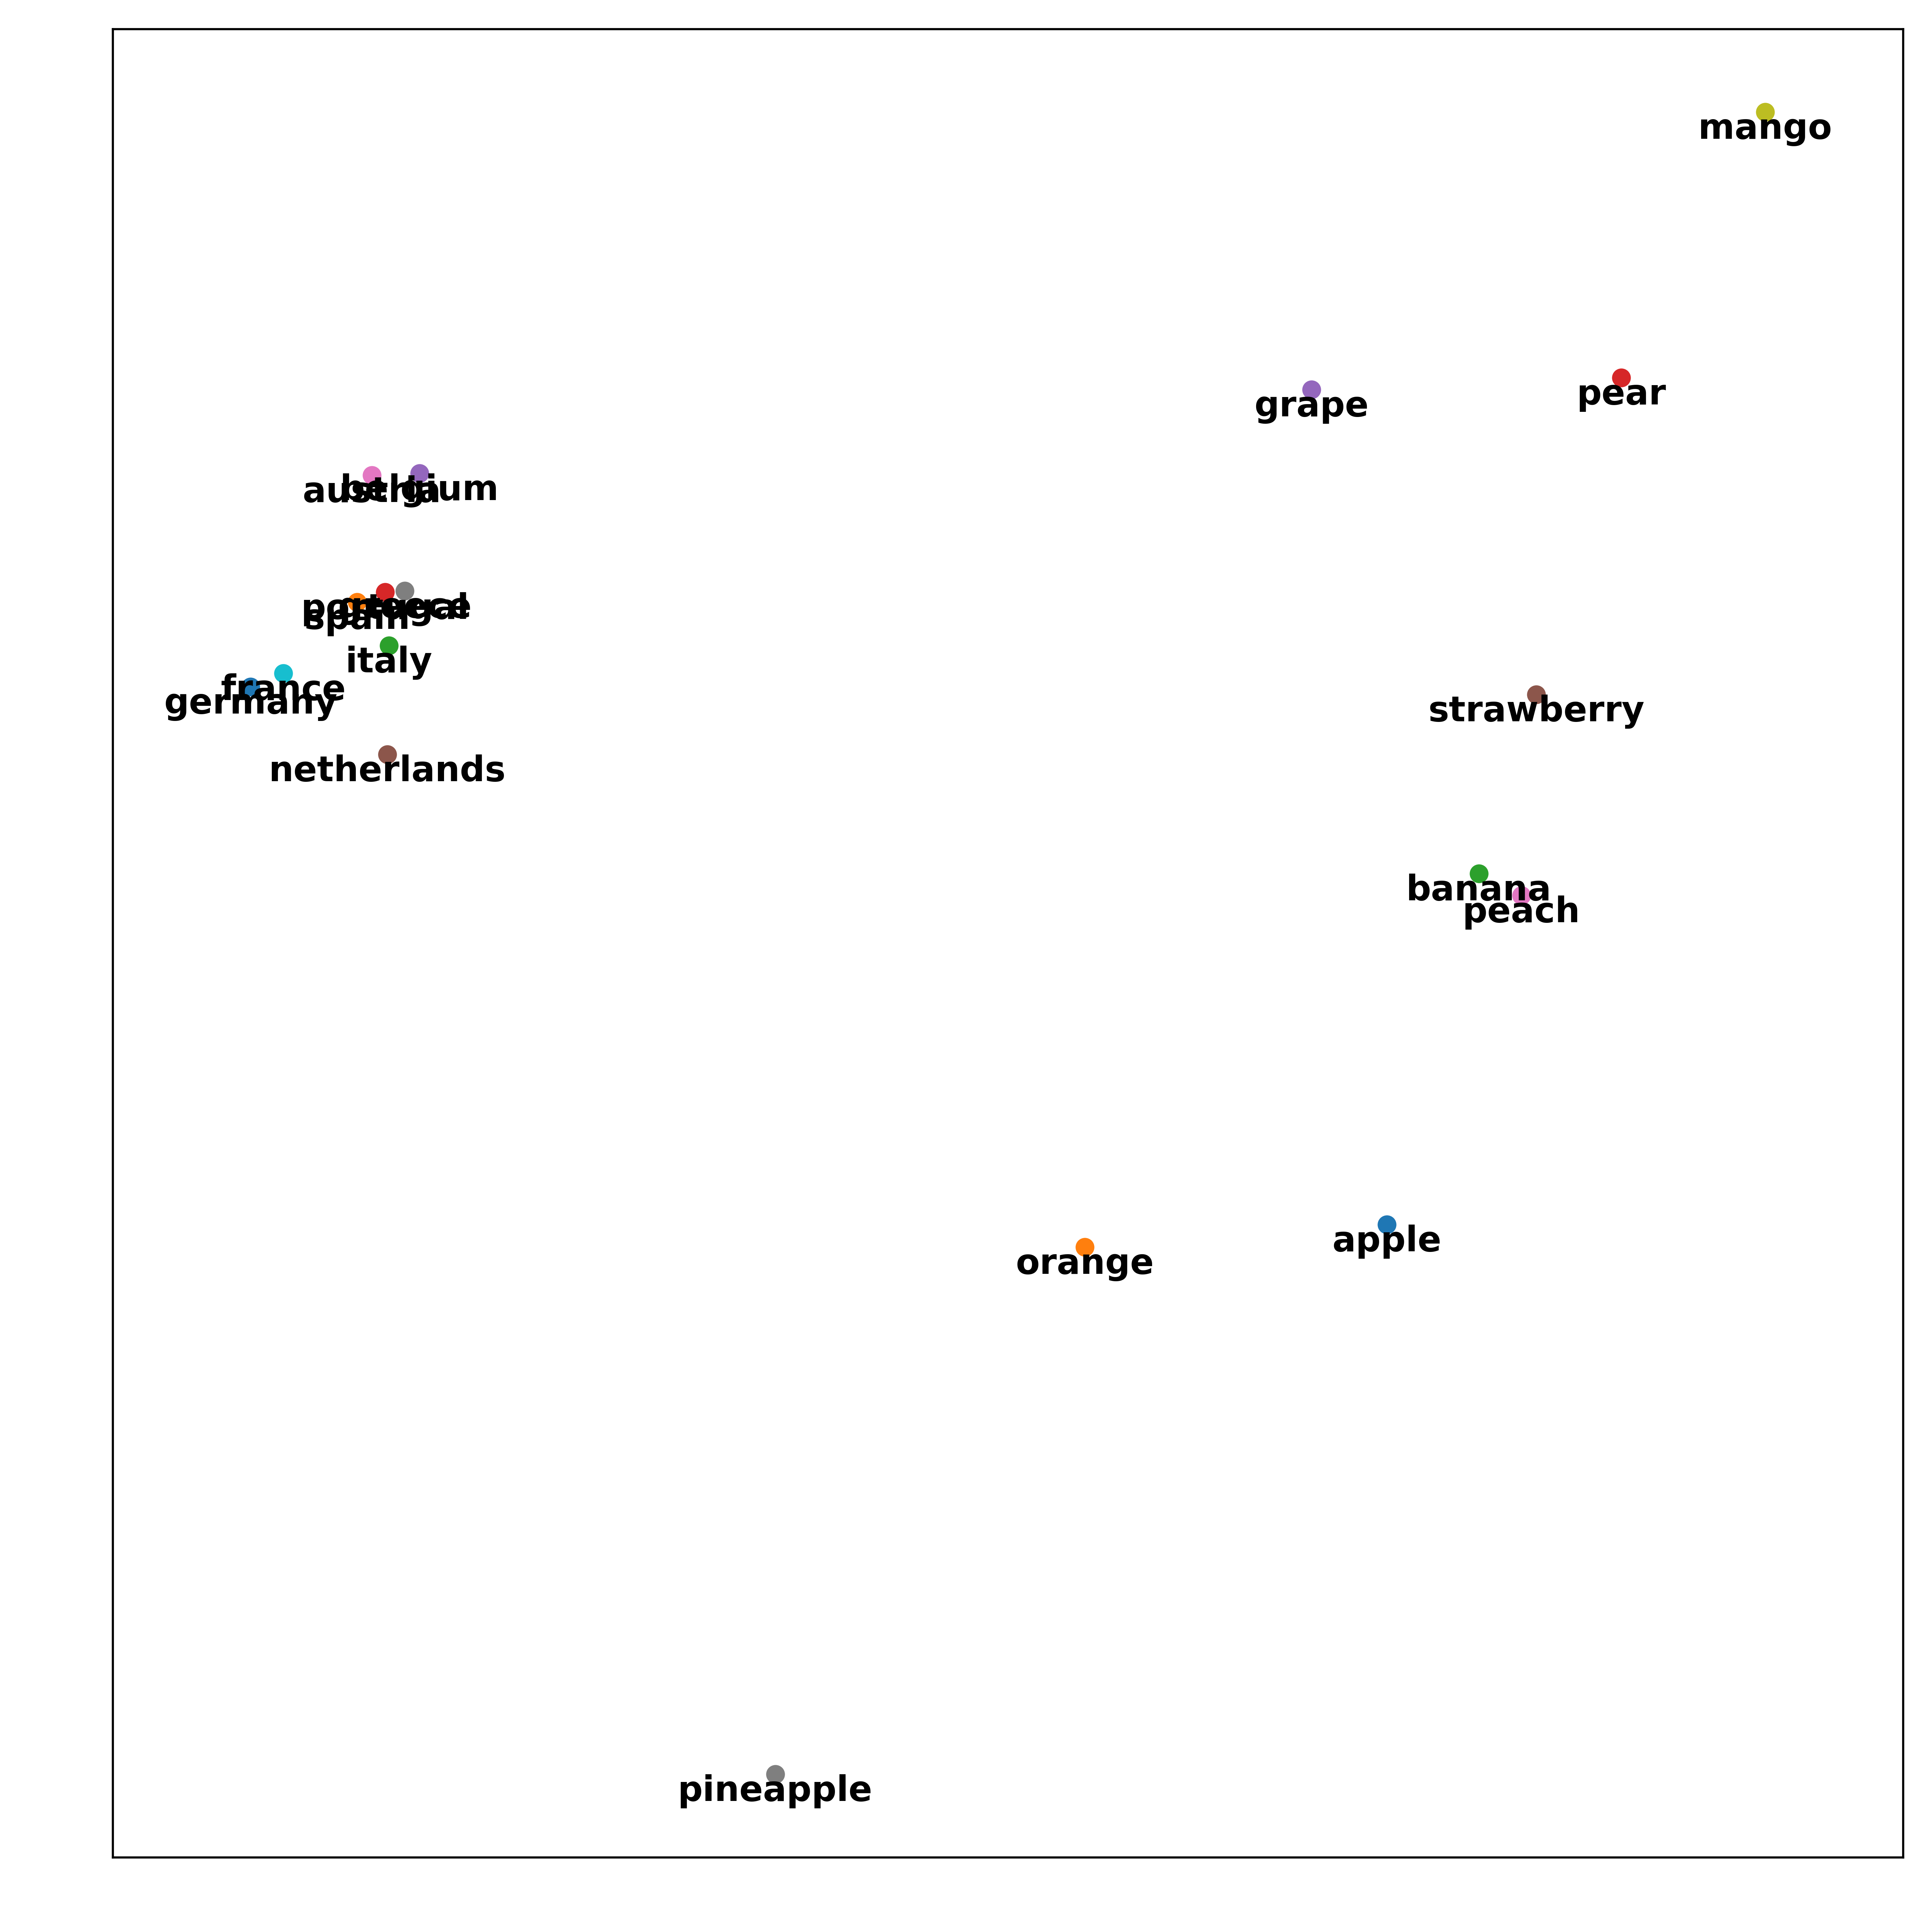
\includegraphics[scale=\myscale,scale=0.3]{figures/projection-pca-1}
	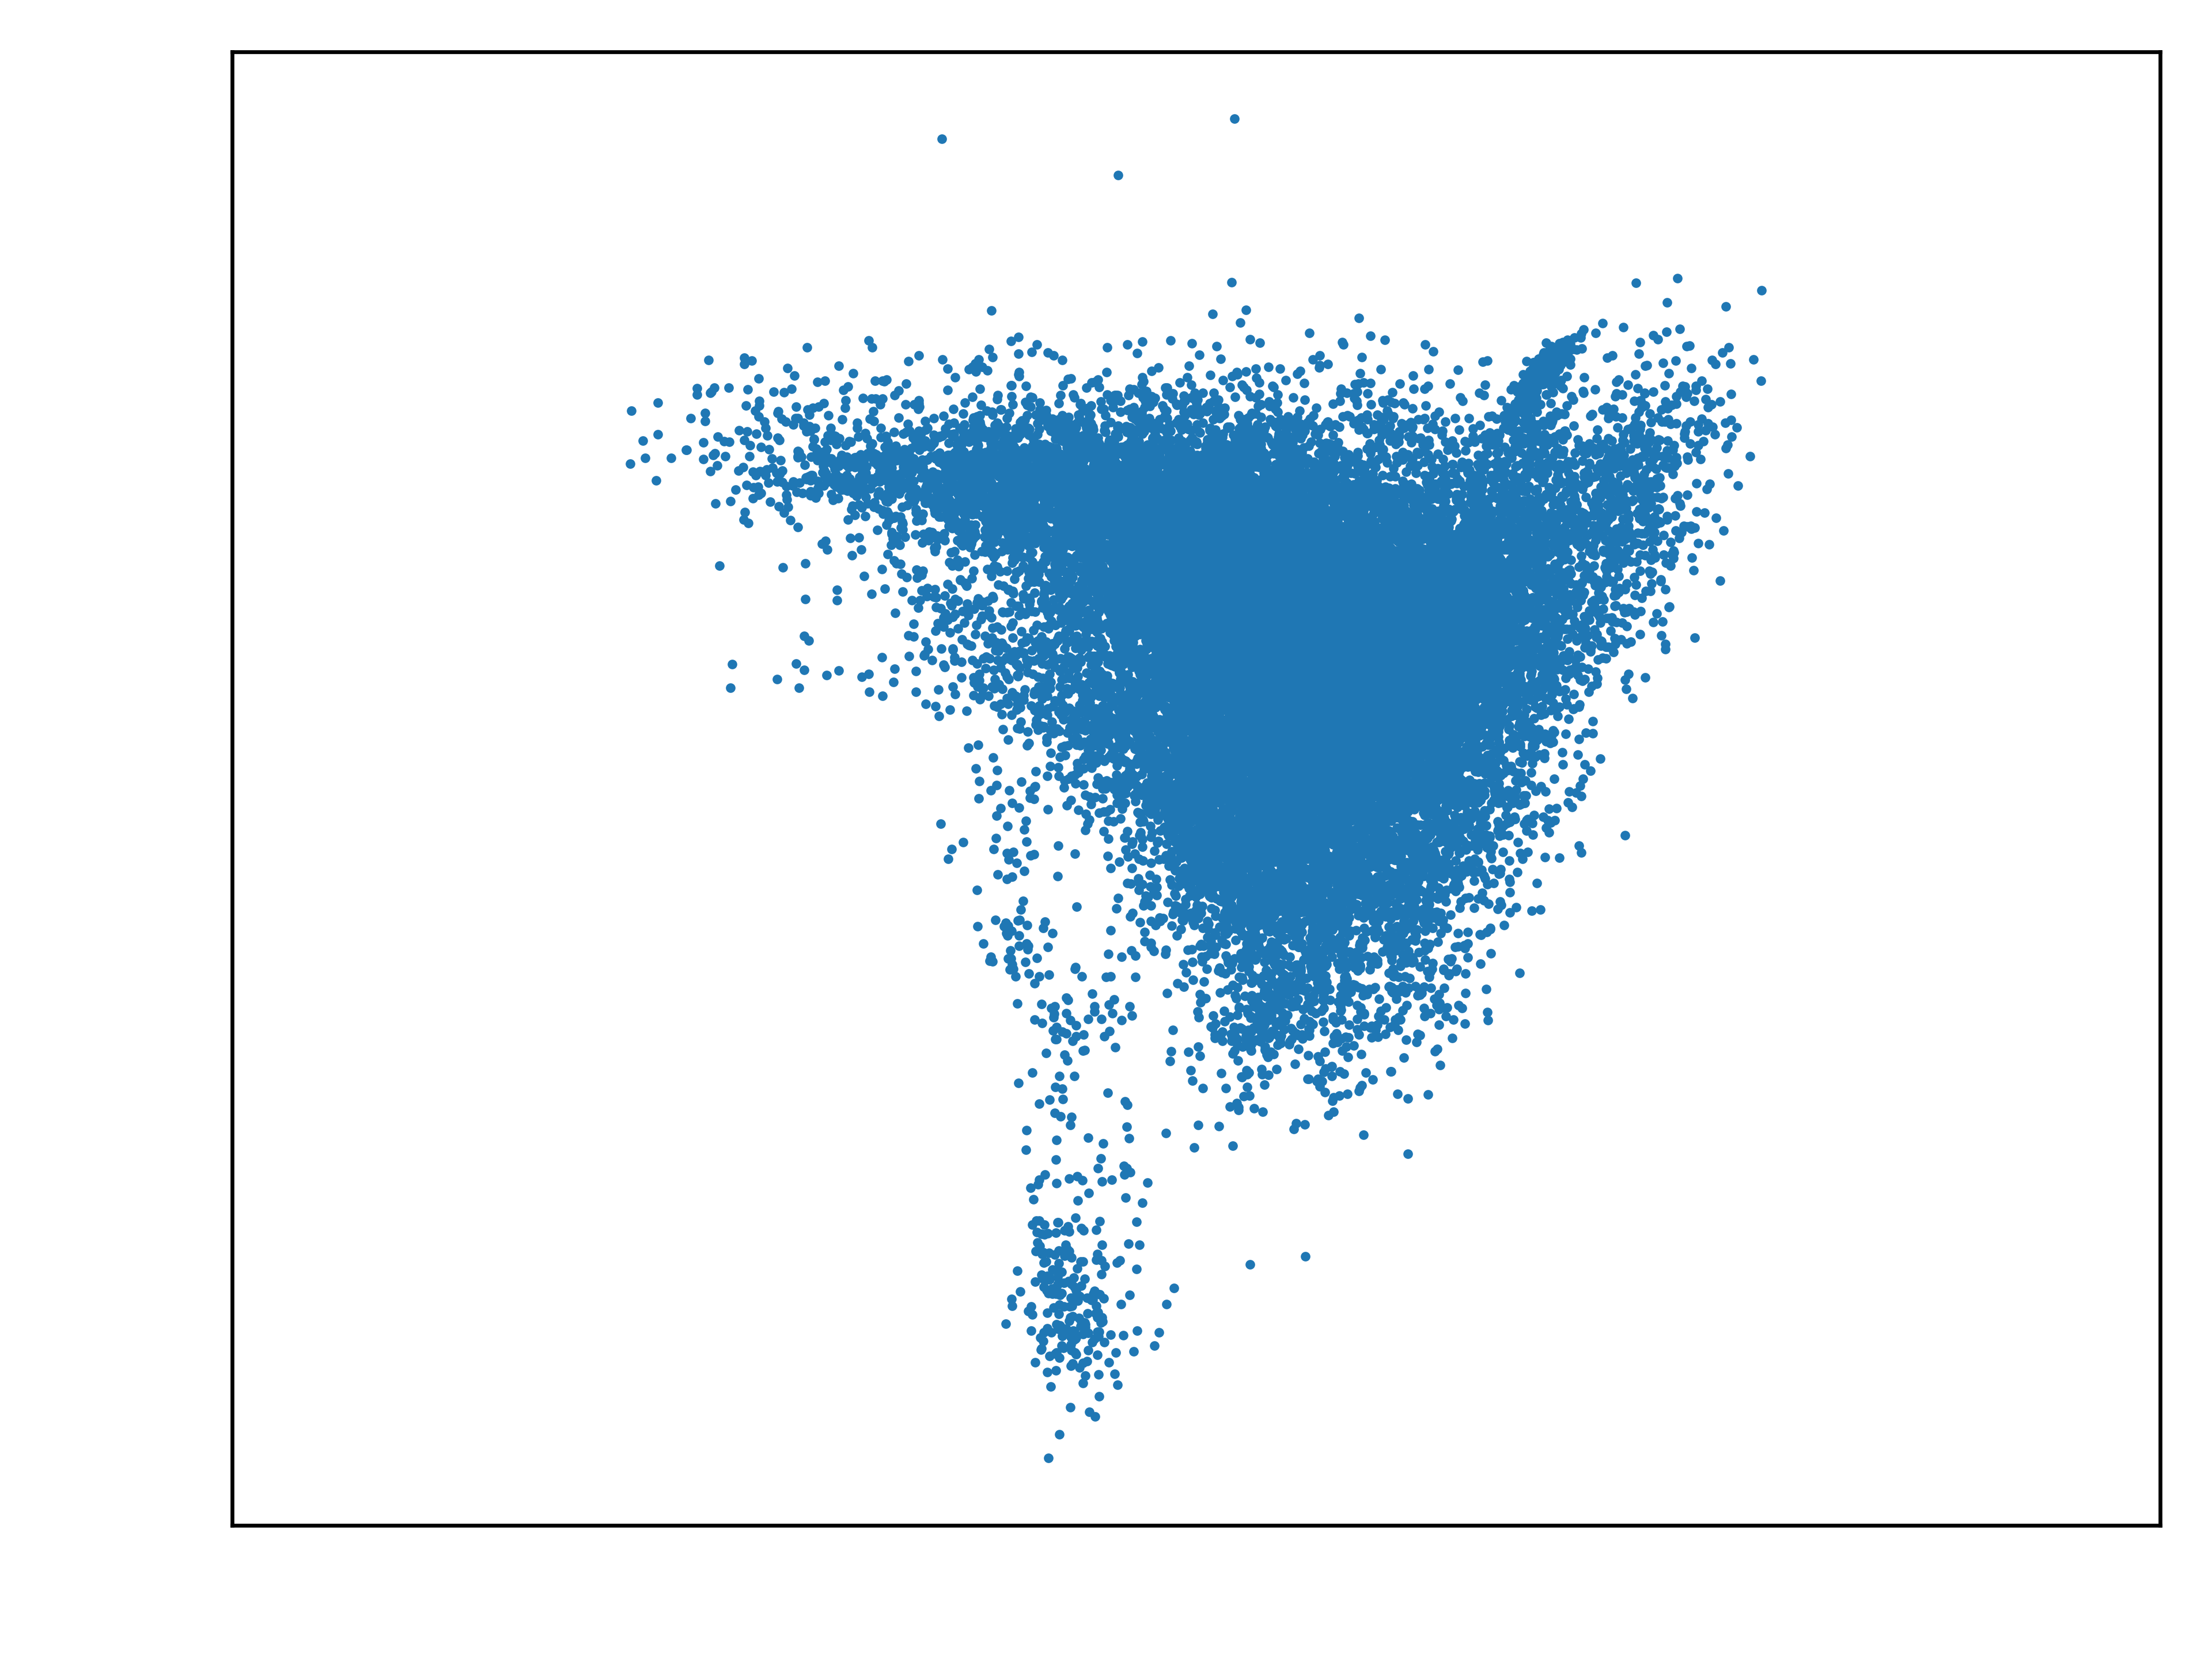
\includegraphics[scale=\myscale,scale=0.5]{figures/projection-pca-4}
\end{center}
\end{exemple}


\begin{exemple}
On considère des mots/tokens de trois thèmes différents : \og{}animaux\fg{}, \og{}métiers\fg{} et \og{}villes\fg{}. Les mots sont clairement séparés selon leur catégorie, cela se voit sur la projection 2D et la projection 3D.

\begin{center}
	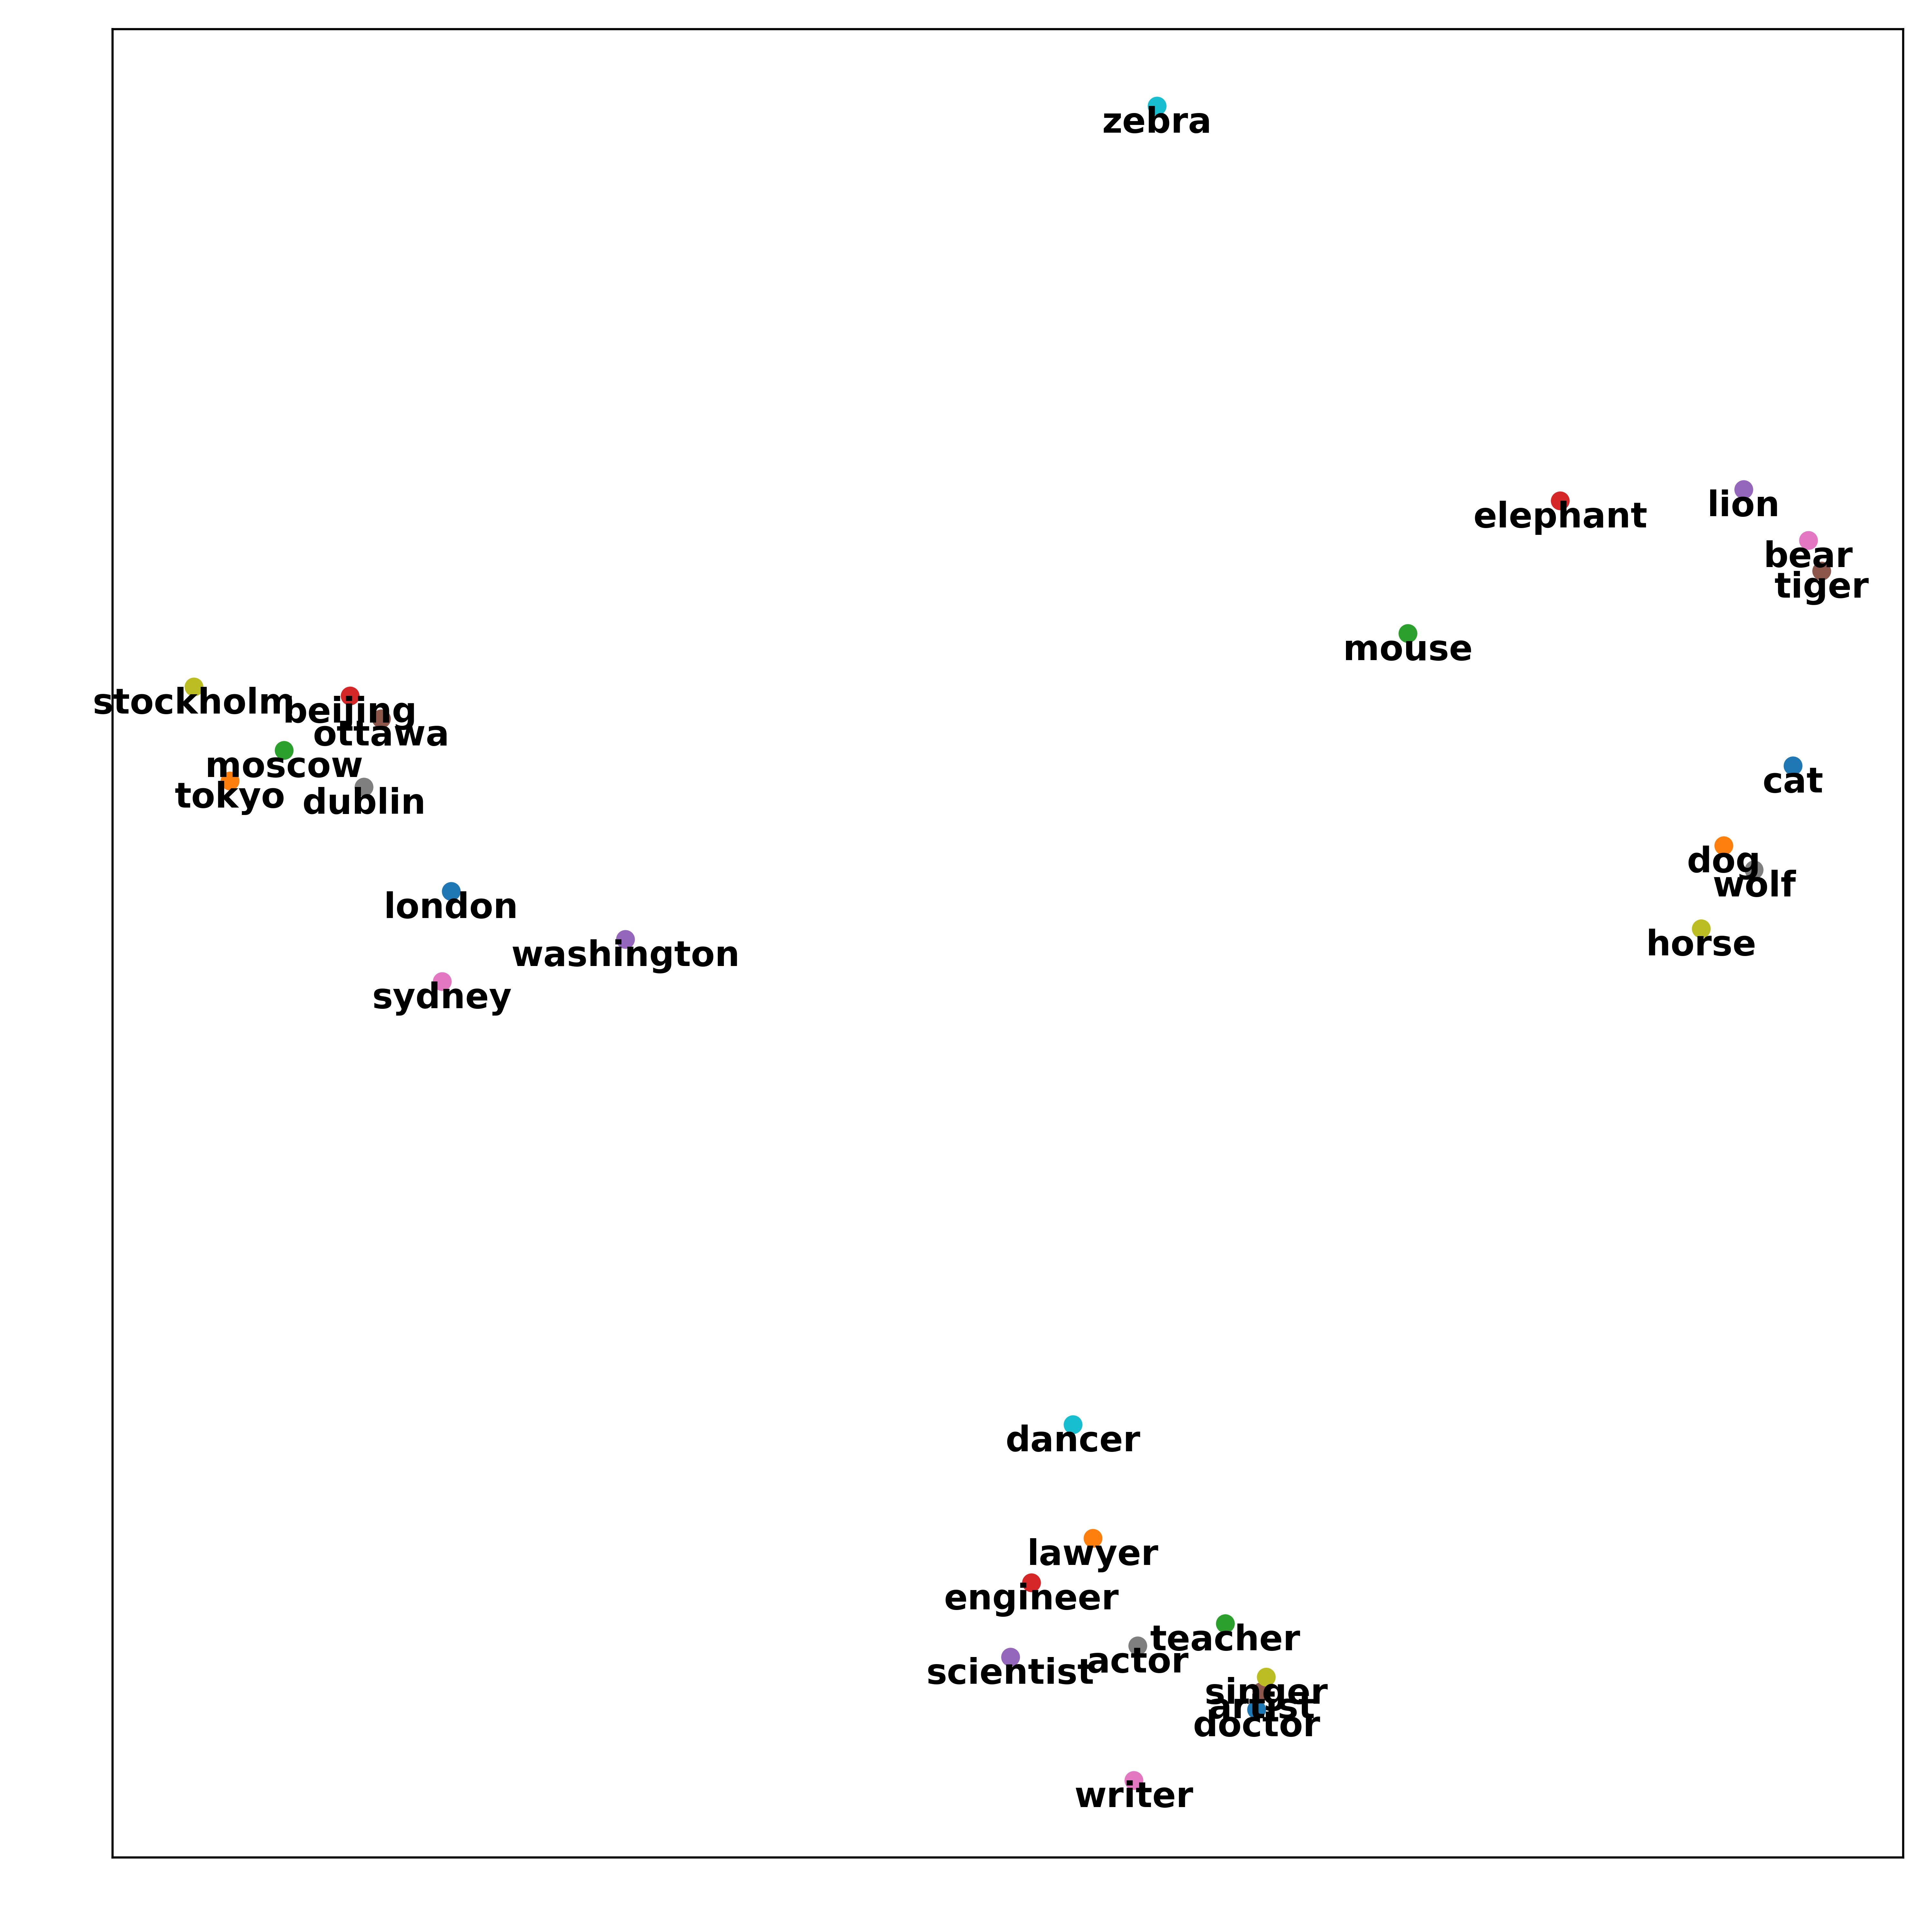
\includegraphics[scale=\myscale,scale=0.3]{figures/projection-pca-2}
	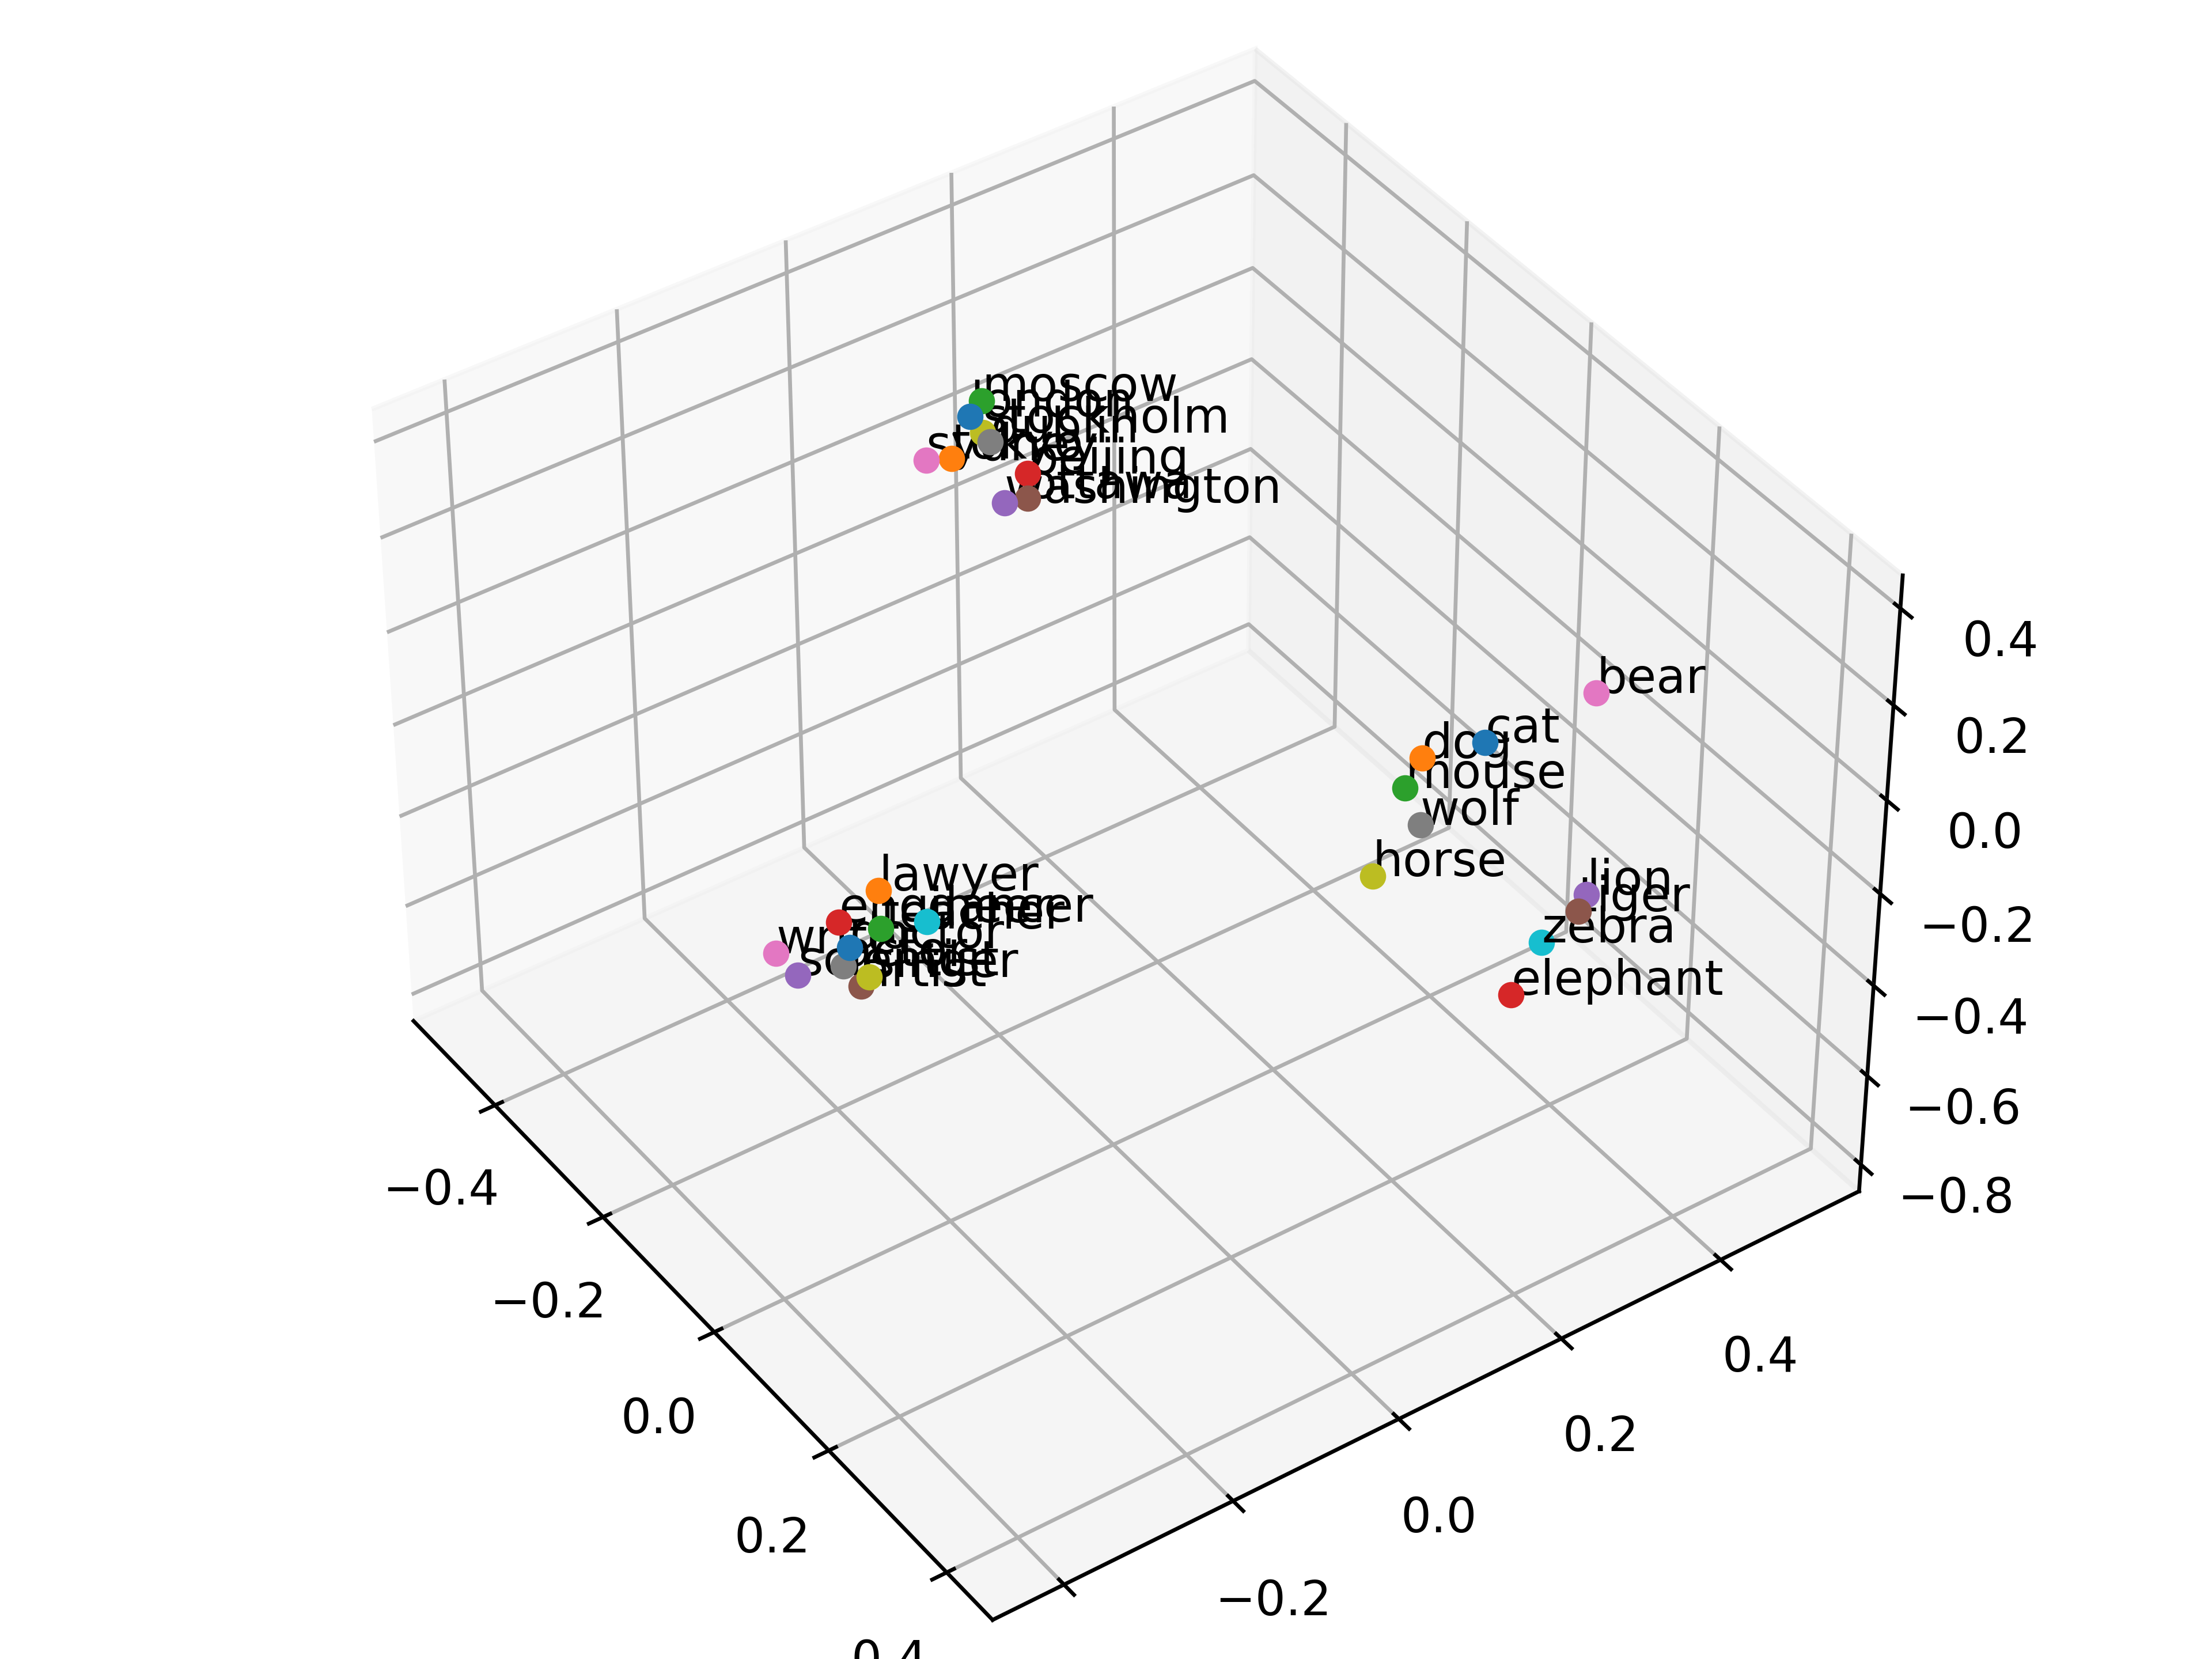
\includegraphics[scale=\myscale,scale=0.5]{figures/projection-pca-3}
\end{center}
\end{exemple}

\bigskip

\textbf{King - Man + Woman = Queen.}
Nous avons vu que les tokens/mots sont plongés dans l'espace en respectant une certaine logique. Voyons à quel point le plongement des tokens permet de comprendre la logique linguistique.
Il existe un phénomène fascinant mais qui relève pour partie d'un mythe, c'est la formule :
$$\text{\mot{king}} - \text{\mot{man}}  + \text{\mot{woman}} = \text{\mot{queen}}$$

Il faut comprendre cette identité sur les vecteurs tokens obtenus par le plongement de chaque mot. Observons la figure de gauche ci-dessous qui est la projection (pca) des plongements des mots \mot{man}, \mot{king}, \mot{woman}, \mot{queen}. On observe en effet que le vecteur qui va de \mot{man} à \mot{king} (c'est donc la projection du vecteur $v_{\text{\mot{king}}} - v_{\text{\mot{man}}}$) est presque égal au vecteur qui va de  \mot{woman} à \mot{queen} (c'est donc la projection du vecteur $v_{\text{\mot{queen}}} - v_{\text{\mot{woman}}}$).

\begin{center}
\begin{minipage}{0.5\textwidth}
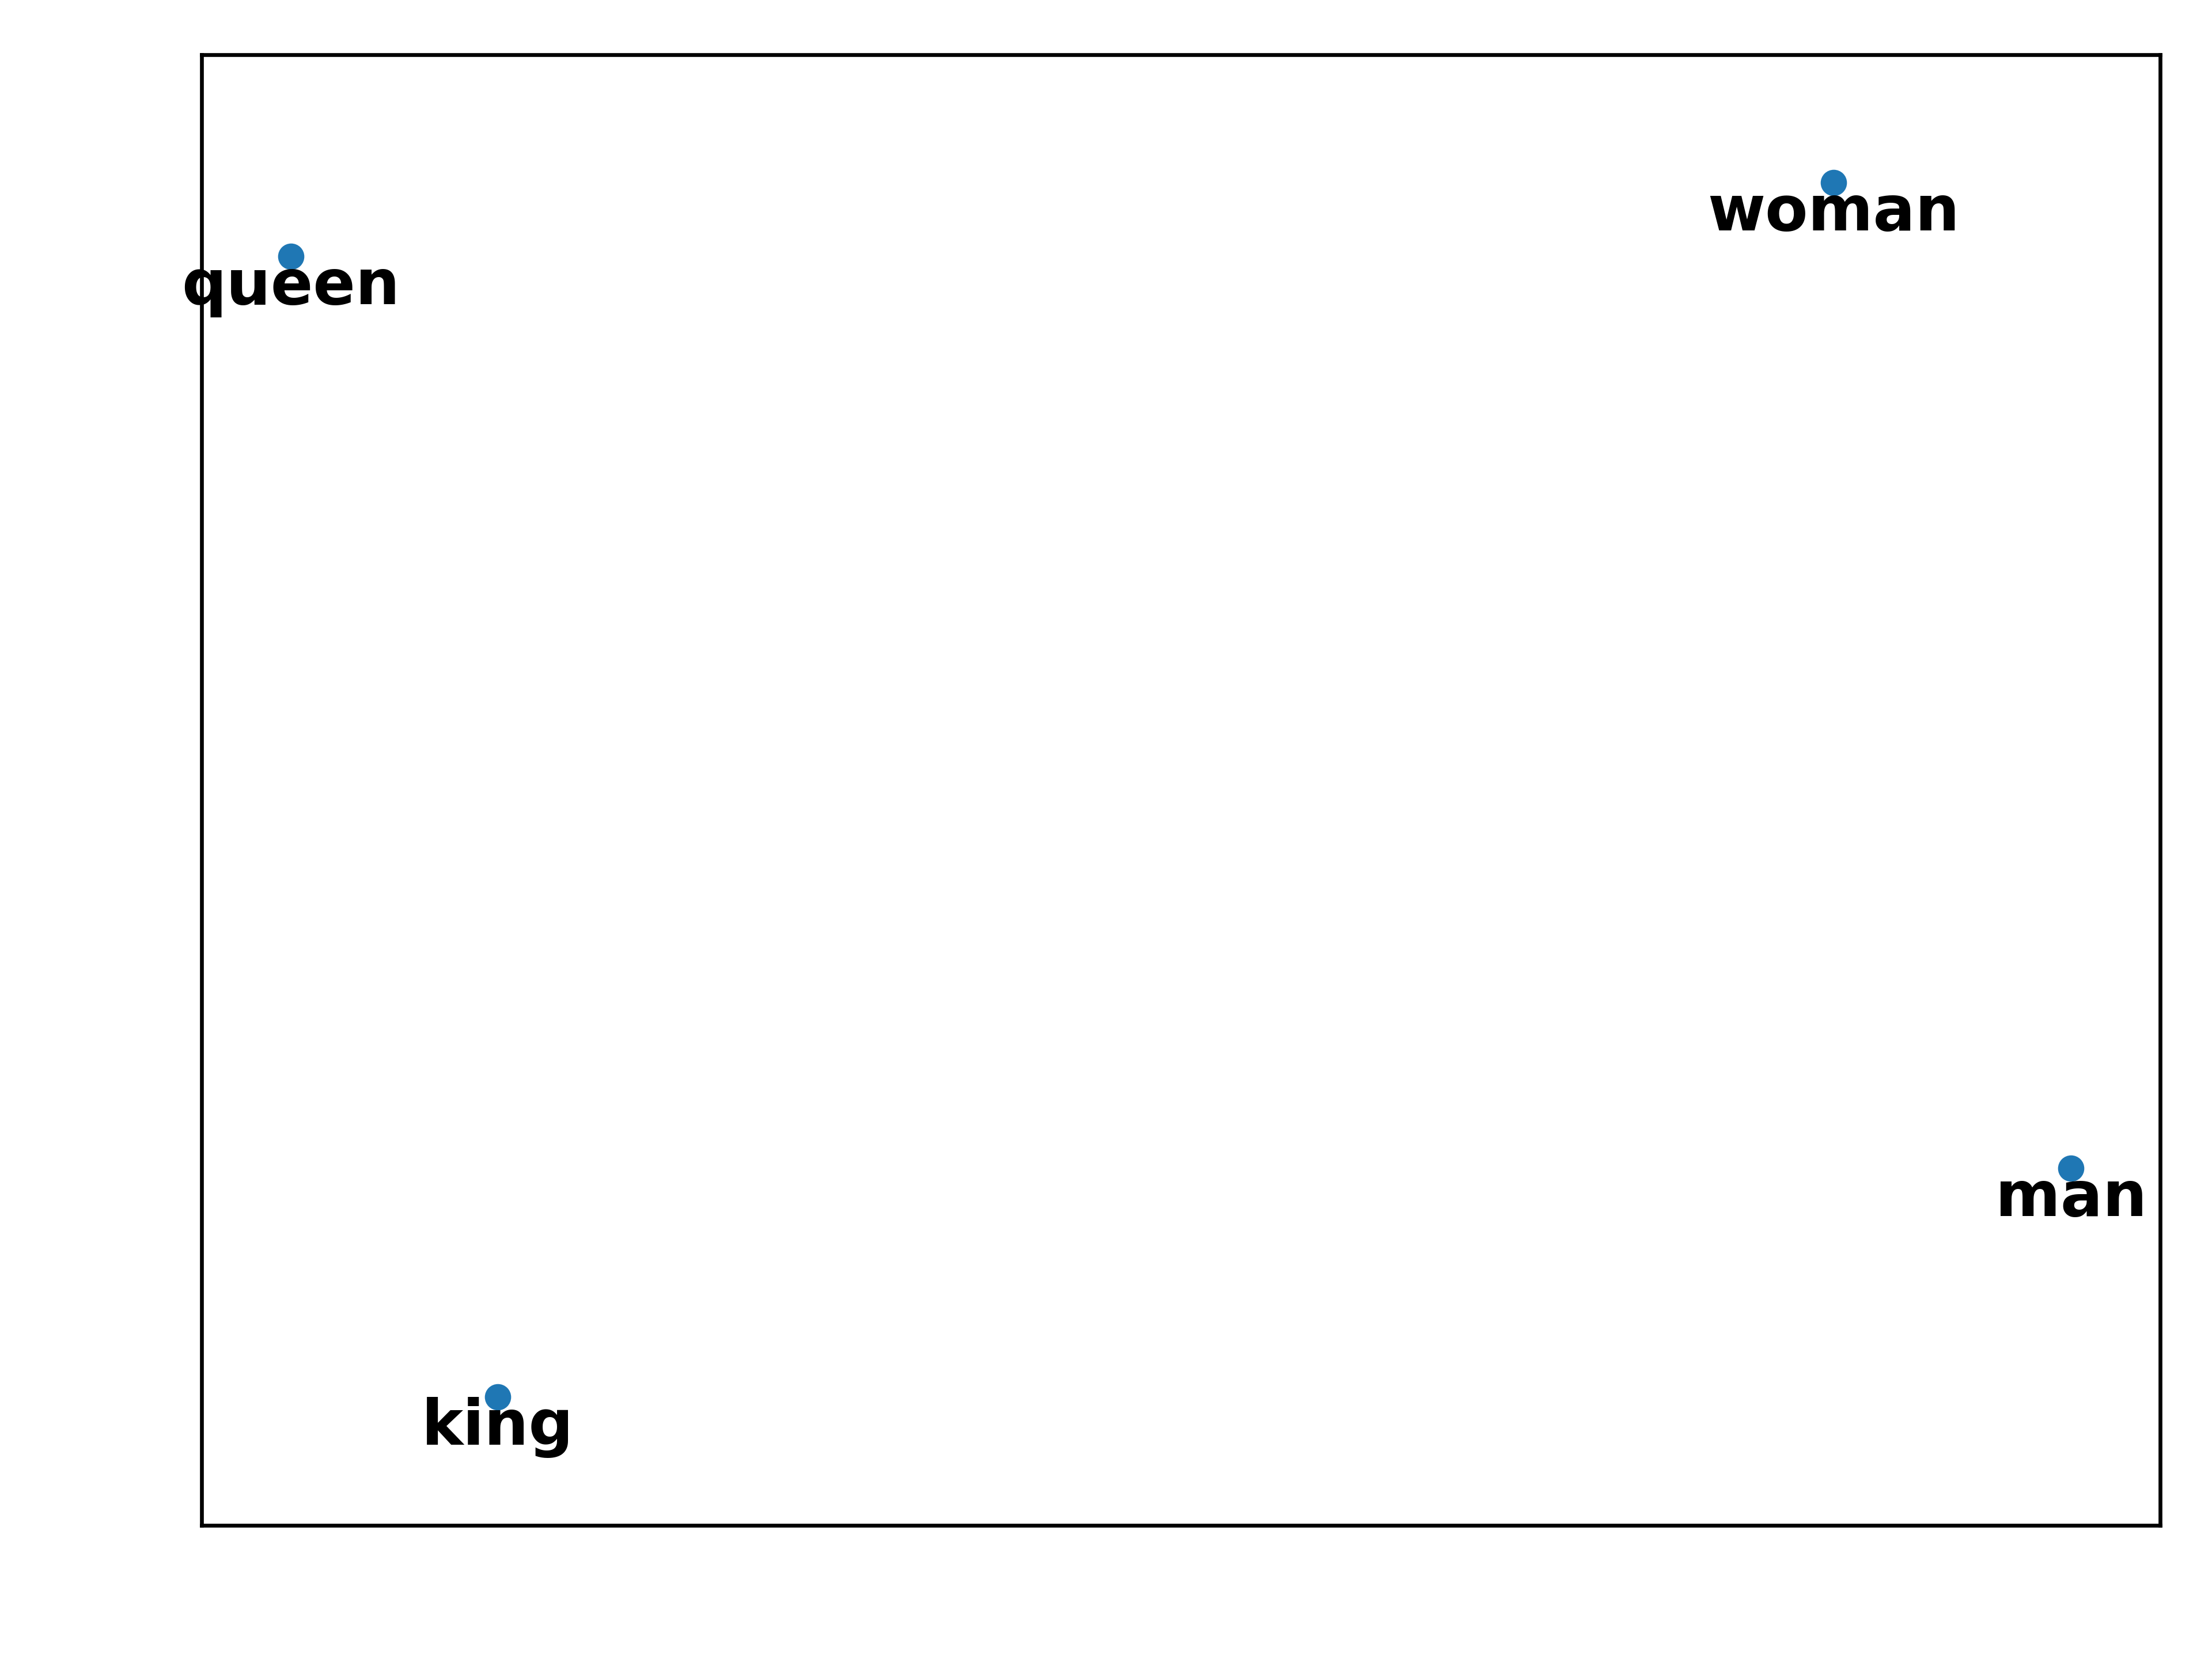
\includegraphics[scale=\myscale,scale=0.5]{figures/projection-pca-5}
\end{minipage}
\begin{minipage}{0.45\textwidth}
\myfigure{1}{ 	
	\tikzinput{projection-03}
} 	
\end{minipage}
\end{center}

On pourrait donc croire que le plongement contient un certaine logique : si pour le terme \mot{king} on remplace le caractère \mot{man} par \mot{woman}, on obtient \mot{queen}.
On retrouve le même phénomène avec les pays et leur capitale. Ci-dessous on passe d'une capitale à son pays par un vecteur à peu près horizontal.
\begin{center}
	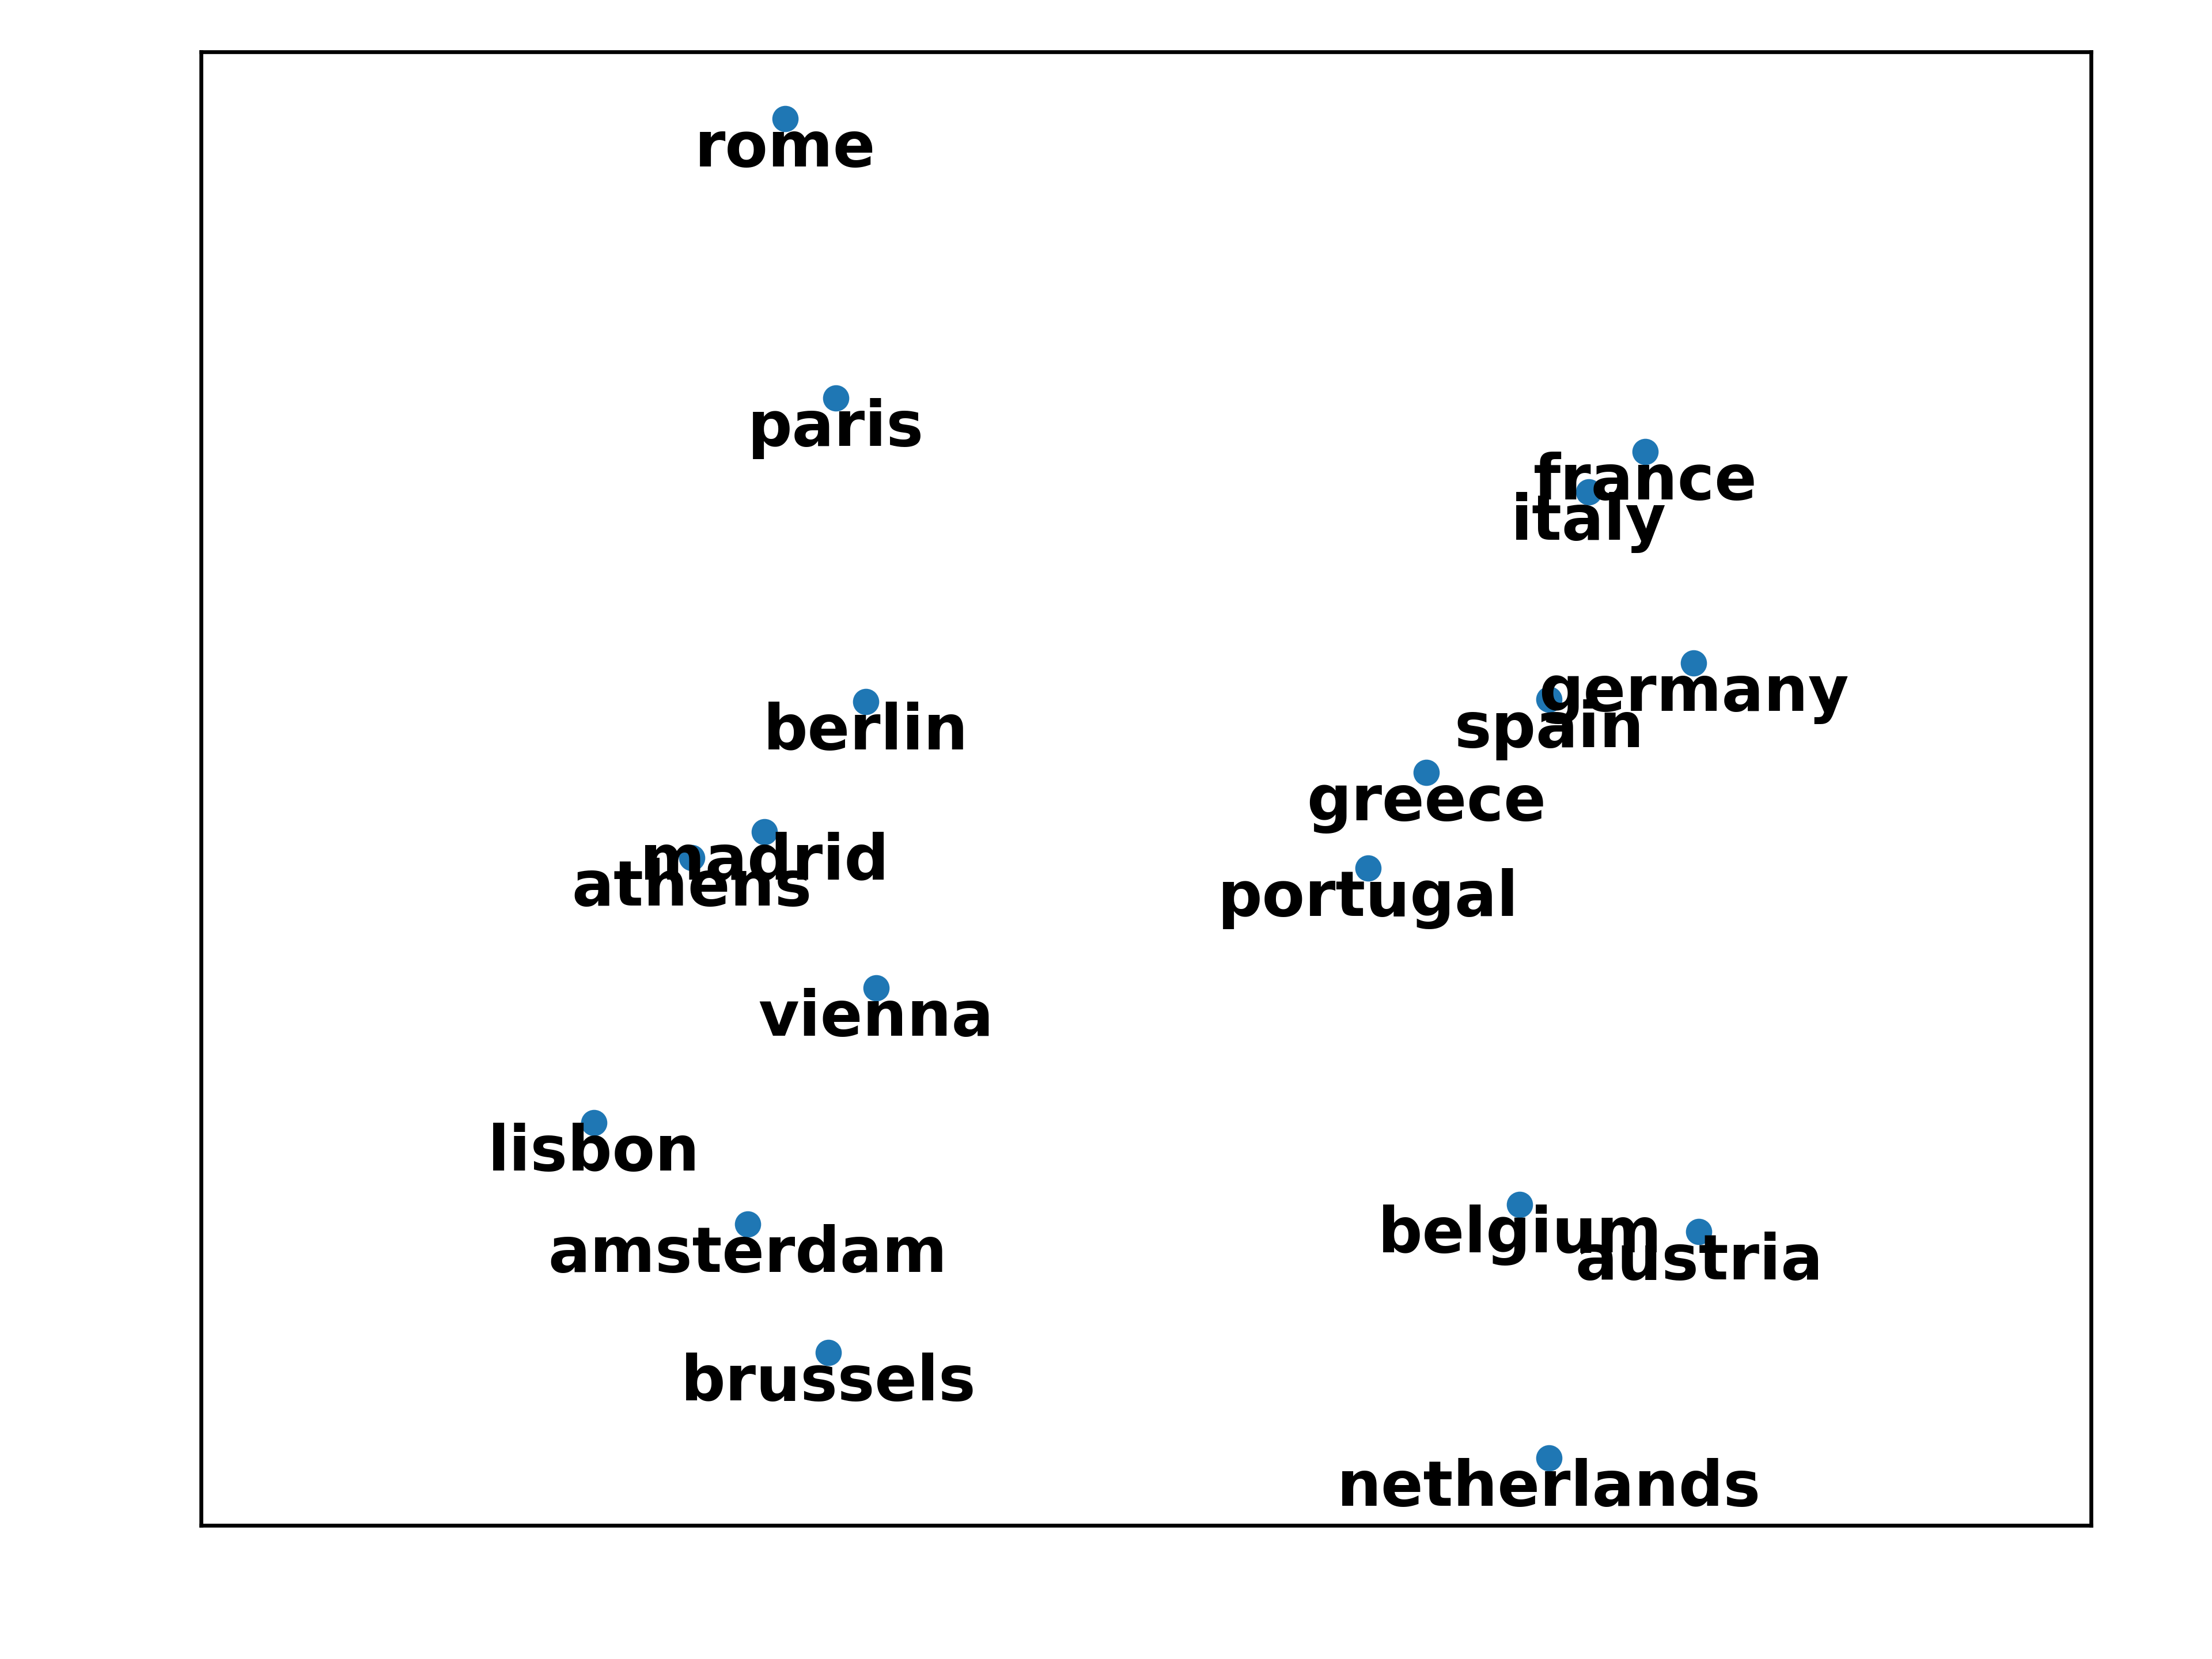
\includegraphics[scale=\myscale,scale=0.6]{figures/projection-pca-6}
\end{center}

En fait ce que l'on voit sur les projections ne reflète pas tout à fait la réalité de ce qui se passe en grande dimension. Si on calcule le vecteur 
$$v =  v_{\text{\mot{king}}} - v_{\text{\mot{man}}} + v_{\text{\mot{woman}}}$$
et que l'on cherche quel vecteur token $v_i$ parmi tous les tokens possibles est le plus proche de $v$ (au sens de la similarité cosinus) les tokens les plus proches sont dans l'ordre :
\mycenterline{\mot{king}, \quad \mot{queen},\quad  \mot{woman},\quad \mot{princess},\quad  \mot{kings},\quad  \mot{queens},\quad \mot{monarch}}
Ainsi, le résultat souhaité, \mot{queen}, n'arrive qu'en deuxième position. Dans ce genre de problème il faut généralement exclure des résultats les termes de départ (ici on exclurait \mot{king}, \mot{man}, \mot{woman}).



%%%%%%%%%%%%%%%%%%%%%%%%%%%%%%%%%%%%%%%%%%%%%%%%%%%%%%%%%%%%%%%%%%%%%
\section{Réalisation d'un plongement}

\index{plongement}

%--------------------------------------------------------------------
\subsection{Plongement des chiffres}

Expliquons le principe de la création d'un plongement à l'aide de l'exemple des chiffres de la base MNIST.
Rappelons que la base MNIST contient des images $28 \times 28$ en niveaux de gris, qu'il faut identifier par une valeur de $0$ à $9$. Il s'agit donc de trouver une fonction $F : \Rr^{784} \to \Rr^{10}$ qui à un vecteur image associe une liste de probabilités (voir la chapitre \og{}Python : tensorflow avec keras - partie 2\fg{}).
Pour déterminer une telle fonction $F$ nous construisons un réseau de neurones comme ci-dessous.

\myfigure{0.7}{ 	
	\tikzinput{neurones-01}
}


\begin{itemize}
	\item En entrée, nous avons un vecteur de taille $N = 784$.
	
	\item Au milieu, nous avons un réseau de neurones non détaillé (avec ou sans couche de convolution), la partie non-détaillée se termine par une couche dense de $n$ neurones, avec par exemple $n=50$. 
	
	\item La dernière couche (couche de sortie) est composée de $10$ neurones, la fonction d'activation est softmax qui est adaptée pour renvoyer des probabilités correspondant au chiffre perçu. On pourrait considérer que $F : \Rr^N \to \Rr^{10}$ est notre plongement mais ce n'est pas le rôle de la couche de sortie qui est de décider d'une valeur entre $0$ et $9$.
	
\end{itemize}
	
Une fois le réseau entraîné, il détecte correctement les chiffres (disons avec une précision $\ge 99\%$). Il est légitime de considérer que cette reconnaissance efficace n'est pas due qu'à la dernière couche et que l'essentiel du travail de catégorisation a déjà eu lieu lors des couches précédentes.
Ainsi les valeurs sortantes de l'avant-dernière couche (qui servent d'entrée à la couche de sortie) ont déjà une certaine pertinence pour déterminer le chiffre.
On considère donc la fonction 
$$\varphi : \Rr^N \to \Rr^n$$
qui à une image associe les valeurs de sortie de l'avant-dernière couche. C'est cette fonction qui sera notre plongement.
Noter que $n$ peut être choisi à la valeur que l'on souhaite, en changeant le nombre de neurones de l'avant-dernière couche.

Voyons l'effet de ce plongement sur une centaine d'images de la base MNIST, après avoir appliqué une analyse en composantes principales pour obtenir une projection 2D et 3D.
\index{donnees@données!MNIST}
\begin{center}
	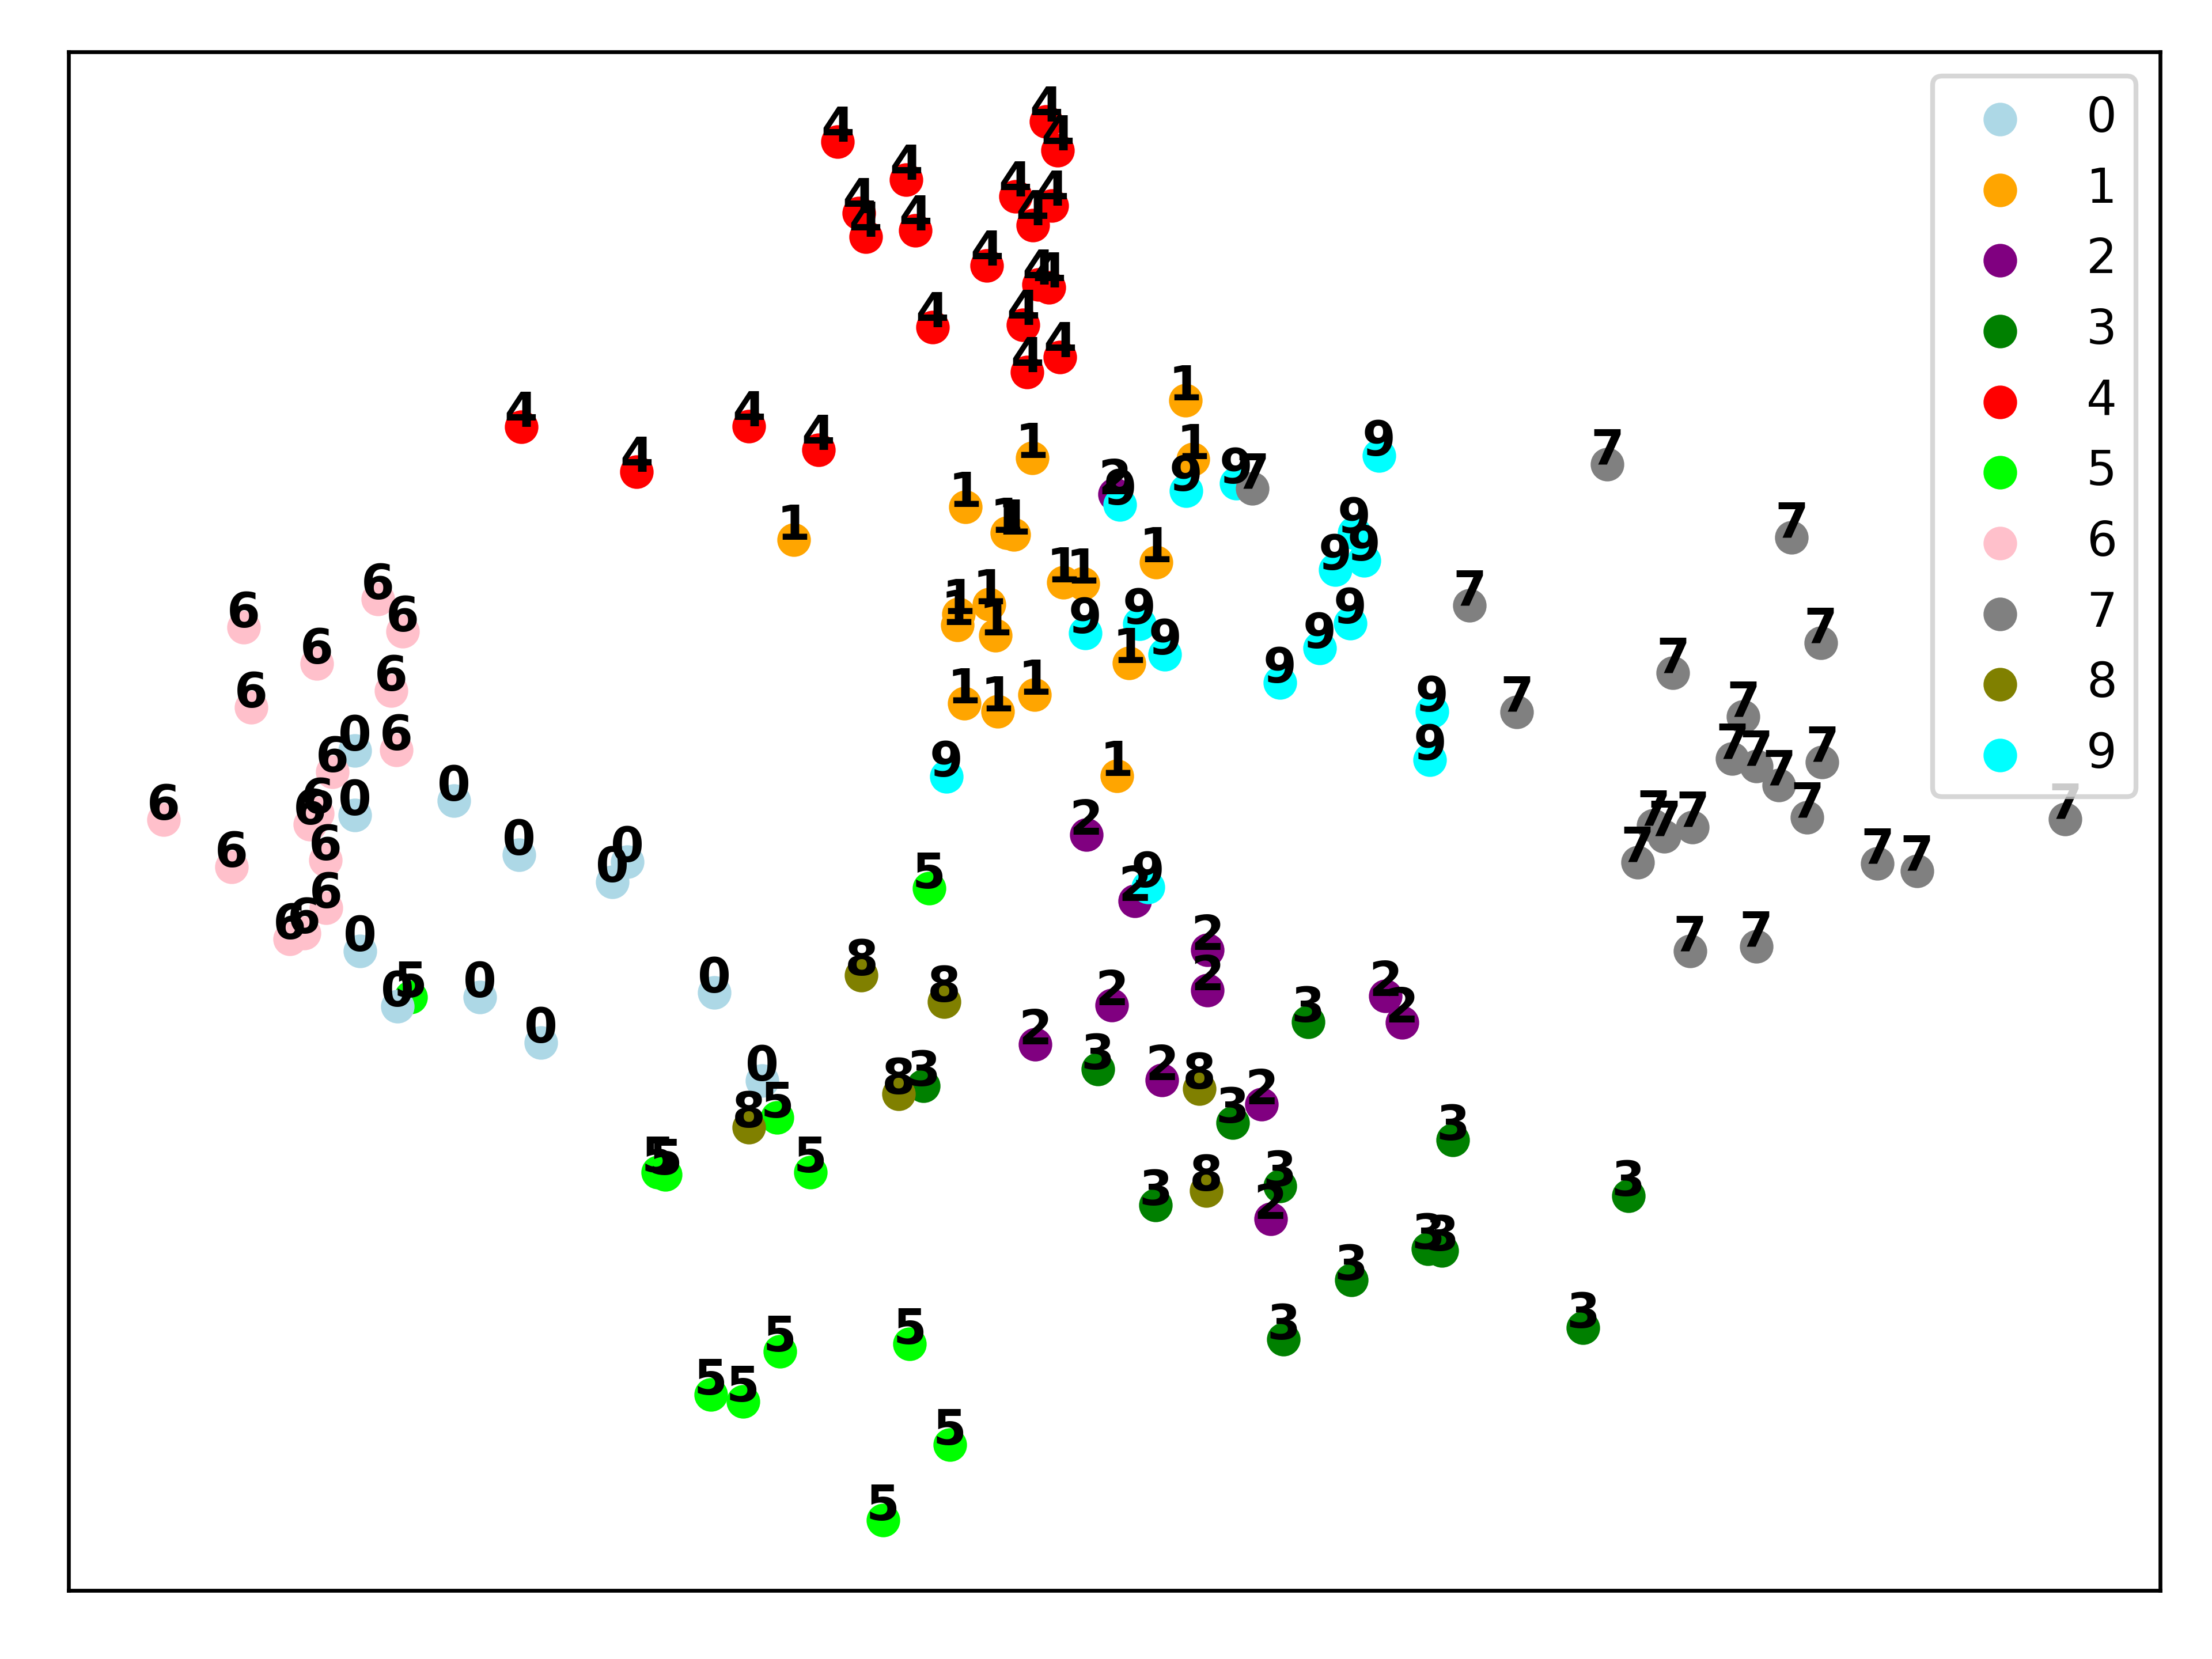
\includegraphics[scale=\myscale,scale=0.5]{figures/mnist-embed-1}
	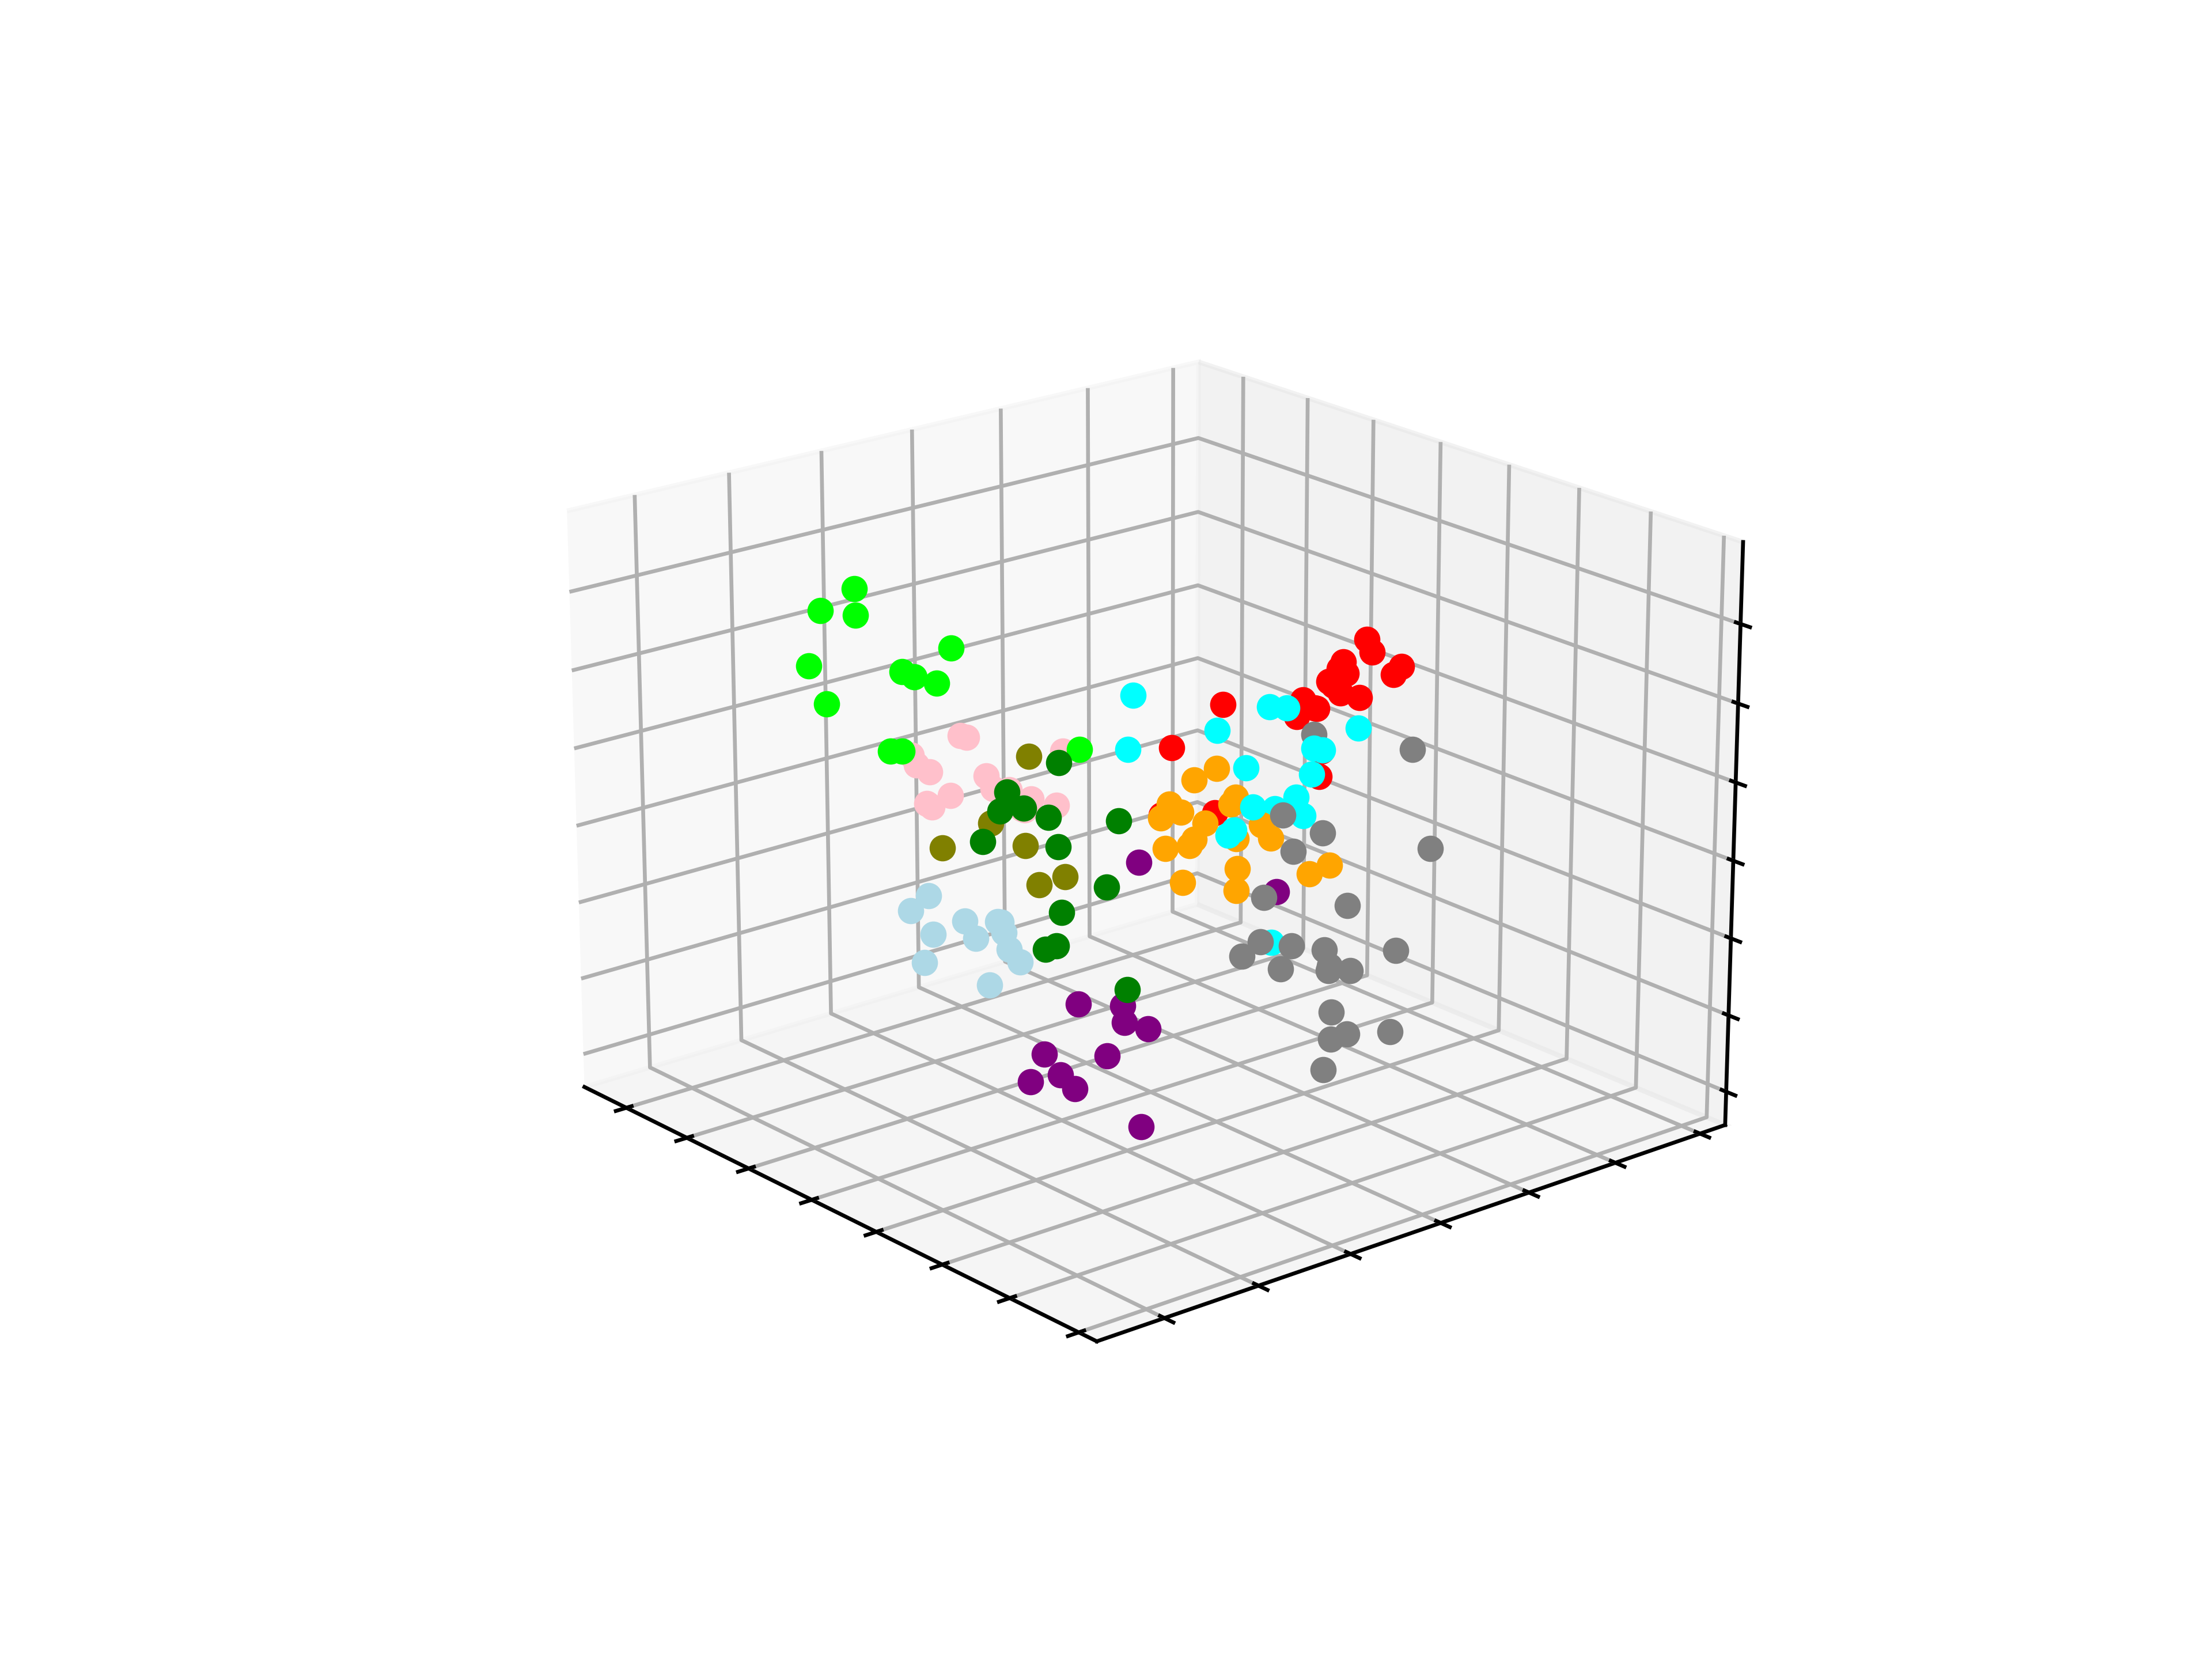
\includegraphics[scale=\myscale,scale=0.7,trim={2cm 2cm 2cm 2cm},clip]{figures/mnist-embed-2}
\end{center}

On visualise bien les différentes catégories de chiffres, il y a cependant des superpositions dans nos projections. Par exemple, dans la projection 2D, les catégories des chiffres $2$ et $3$ s’entremêlent mais on constate que dans la projection 3D ces catégories sont assez bien séparées. On rappelle qu'une projection 2D ou 3D ne reflète que très partiellement la réalité d'un espace de grande dimension, ici $n=50$. 

%--------------------------------------------------------------------
\subsection{Co-occurrence}

\index{co-occurrence}

Nous expliquons maintenant comment réaliser un plongement des tokens à partir d'un corpus. Nous allons réaliser un plongement simple mais tout de même efficace.

La première partie consiste à reprendre nos statistiques linguistiques des sections précédentes. 
À partir du corpus, on définit $N$ tokens. Ensuite on définit la matrice des co-occurrences. C'est une matrice de taille $N \times N$ dans laquelle à la position (colonne $i$, ligne $j$) on insère le nombre de co-occurrences de (mot$i$, mot$j$) c'est-à-dire mot$i$ suivi de mot$j$.

Voici un exemple minimaliste avec les $N=4$ tokens \mot{le}, \mot{et}, \mot{chat}, \mot{chien} (dans cet ordre). Imaginons que la matrice de co-occurrence soit :
\begin{center}
\begin{tabular}{lcccc}
	             & $i=1$ \mot{le} & $i=2$ \mot{et} & $i=3$ \mot{chat} & $i=4$ \mot{chien} \\
$j=1$ \mot{le}   & 0  & 10 & 1  & 0 \\
$j=2$ \mot{et}   & 0  & 0  & 8  & 5 \\
$j=3$ \mot{chat} & 6  & 2  & 0  & 0 \\
$j=4$ \mot{chien}& 4  & 3  & 1  & 0 \\
\emph{Total}     & \emph{10} & \emph{15} & \emph{10} & \emph{5} \\	
\end{tabular}
\end{center}
Chaque occurrence de \og{}\mot{le chat}\fg{} dans le texte correspond à la paire (\mot{le}, \mot{chat}) et contribue à $+1$ à la place $(i=1,j=3)$ de la matrice de co-occurrence. Ici dans le texte il y a eu $6$ occurrences de \og{}\mot{le chat}\fg{}.

Pour obtenir la matrice des probabilités, il faut pour chaque mot$i$, calculer la probabilité que le mot suivant soit mot$j$.
Cette probabilité $p_{ij}$ (à la colonne $i$, ligne $j$) se calcule par :
$$p_{ij} = \frac{\text{nombre d'occurrences de la paire (mot$i$, mot$j$)}}{\text{nombre d'occurrences de mot$i$}}.$$
	
Pour notre exemple minimaliste la matrice serait :
$$P = \begin{pmatrix}
 \frac{0}{10}  & \frac{10}{15} & \frac{1}{10} & \frac{0}{5} \\
 \frac{0}{10}  & \frac{0}{15}  & \frac{8}{10} & \frac{5}{5} \\
 \frac{6}{10}  & \frac{2}{15}  & \frac{0}{10} & \frac{0}{5} \\
 \frac{4}{10}  & \frac{3}{15}  & \frac{1}{10} & \frac{0}{5} \\	
\end{pmatrix}.$$


\begin{exemple}
Reprenons le corpus \emph{Reuters}. Parmi tous les mots (en minuscules, de longueur $>1$), on travaille sur le vocabulaire  des $N=500$ mots les plus fréquents qui seront nos tokens.

Les cinq premiers mots les plus fréquents sont : 
\mycenterline{\mot{the},\quad \mot{of},\quad \mot{to},\quad \mot{in},\quad \mot{and}.}

La matrice de co-occurrence est une matrice de taille $N \times N$, donc ici $500 \times 500$ :
$$M = \begin{pmatrix}
 20 & 6834 & 2482 & 6757 & 1575 & \ldots \\
  0 &  11  &  0   & 1 &  31     & \ldots \\
  0 &   2  &  8   & 2 & 211     &\ldots \\
  2 &   4  &  6   & 1 & 132     &\ldots \\
  0 &   1  & 11   & 23 &   5    & \ldots \\
  \vdots & \vdots & \vdots & \vdots & \vdots & \ddots \\
\end{pmatrix}.$$
Par exemple, la deuxième colonne correspond au nombre d'occurrences du mot qui suit \mot{of}. 
Il y a par exemple $6834$ occurrences de la paire (\mot{of}, \mot{the}).
La matrice $P$ des probabilités (de même taille) s'en déduirait facilement.
\end{exemple}

Ce que l'on retient, c'est que la colonne $P_i$ de la matrice $P$ contient la liste des probabilités pour chaque mot à la suite de mot$i$. Autrement dit, comme $P_i = P e_i$, $P$ est la matrice de l'application linéaire $G$ définie par :
$$
\begin{array}{rccc}
G : & \Rr^N & \longmapsto & \Rr^N \\
    & e_i   & \longmapsto & P_i
\end{array}
$$




%--------------------------------------------------------------------
\subsection{Plongement}


Nous allons maintenant réaliser un plongement $\varphi : \Rr^N \to \Rr^n$ à partir de la matrice $P$ des probabilités.
Construisons un réseau de neurones :
\begin{itemize}
	\item En entrée nous avons un vecteur de taille $N$.
	
	\item Ensuite nous avons un réseau de neurones (plus ou moins complexe), ce réseau se termine par une couche dense de $n$ neurones, avec par exemple $n=768$ ou $n=1024$. 
	
	\item On ajoute enfin une couche de sortie composée de $N$ neurones (autant que la dimension d'entrée) associés à la fonction d'activation softmax.
\end{itemize}

\myfigure{0.7}{ 	
	\tikzinput{neurones-02}
}

Ce réseau réalise donc une fonction $F : \Rr^N \to \Rr^N$.
On entraîne ce réseau afin que $F$ soit le plus proche possible de $G$, c'est-à-dire que pour chaque $i$ on ait $F(e_i) \simeq P_i$. Ce réseau est donc adapté à prédire le mot suivant.

Une fois ce réseau entraîné, on considère la fonction $\varphi : \Rr^N \to \Rr^n$ qui à un vecteur $e_i$ de la base canonique associe les valeurs en sortie de la couche dense de $n$ neurones. C'est cette fonction qui sera notre plongement. (Une fois $\varphi$ définie sur la base canonique, elle se prolonge par linéarité à tout $\Rr^N$.)

Comme pour le plongement des chiffres, le fait que le réseau soit entraîné à reconnaître le successeur d'un mot signifie que les valeurs en sortie de l'avant-dernière couche de $n$ neurones sont déjà une certaine représentation des mots. 

\begin{exemple}
Finalisons le plongement issu des dépêches \emph{Reuters}.
On crée un réseau de neurones avec $N=500$ entrées,
puis une ou deux couches denses ou de convolutions, suivies ensuite d'une couche dense de $n=50$ neurones (l'avant-dernière couche), puis une couche de sortie de $N=500$ neurones avec la fonction d'activation softmax.

\myfigure{0.7}{ 	
	\tikzinput{neurones-03}
}

On entraîne ce réseau pour que $F(e_i) \simeq P_i$ pour chaque $i$.
En récupérant les valeurs en sortie de la couche des $n$ neurones, on définit notre plongement $\varphi : \Rr^N \to \Rr^n$.

On teste notre plongement sur des catégories de mots et on projette le résultat sur le plan.
Voici un exemple avec les mois de l'année et des nombres.

\begin{center}
	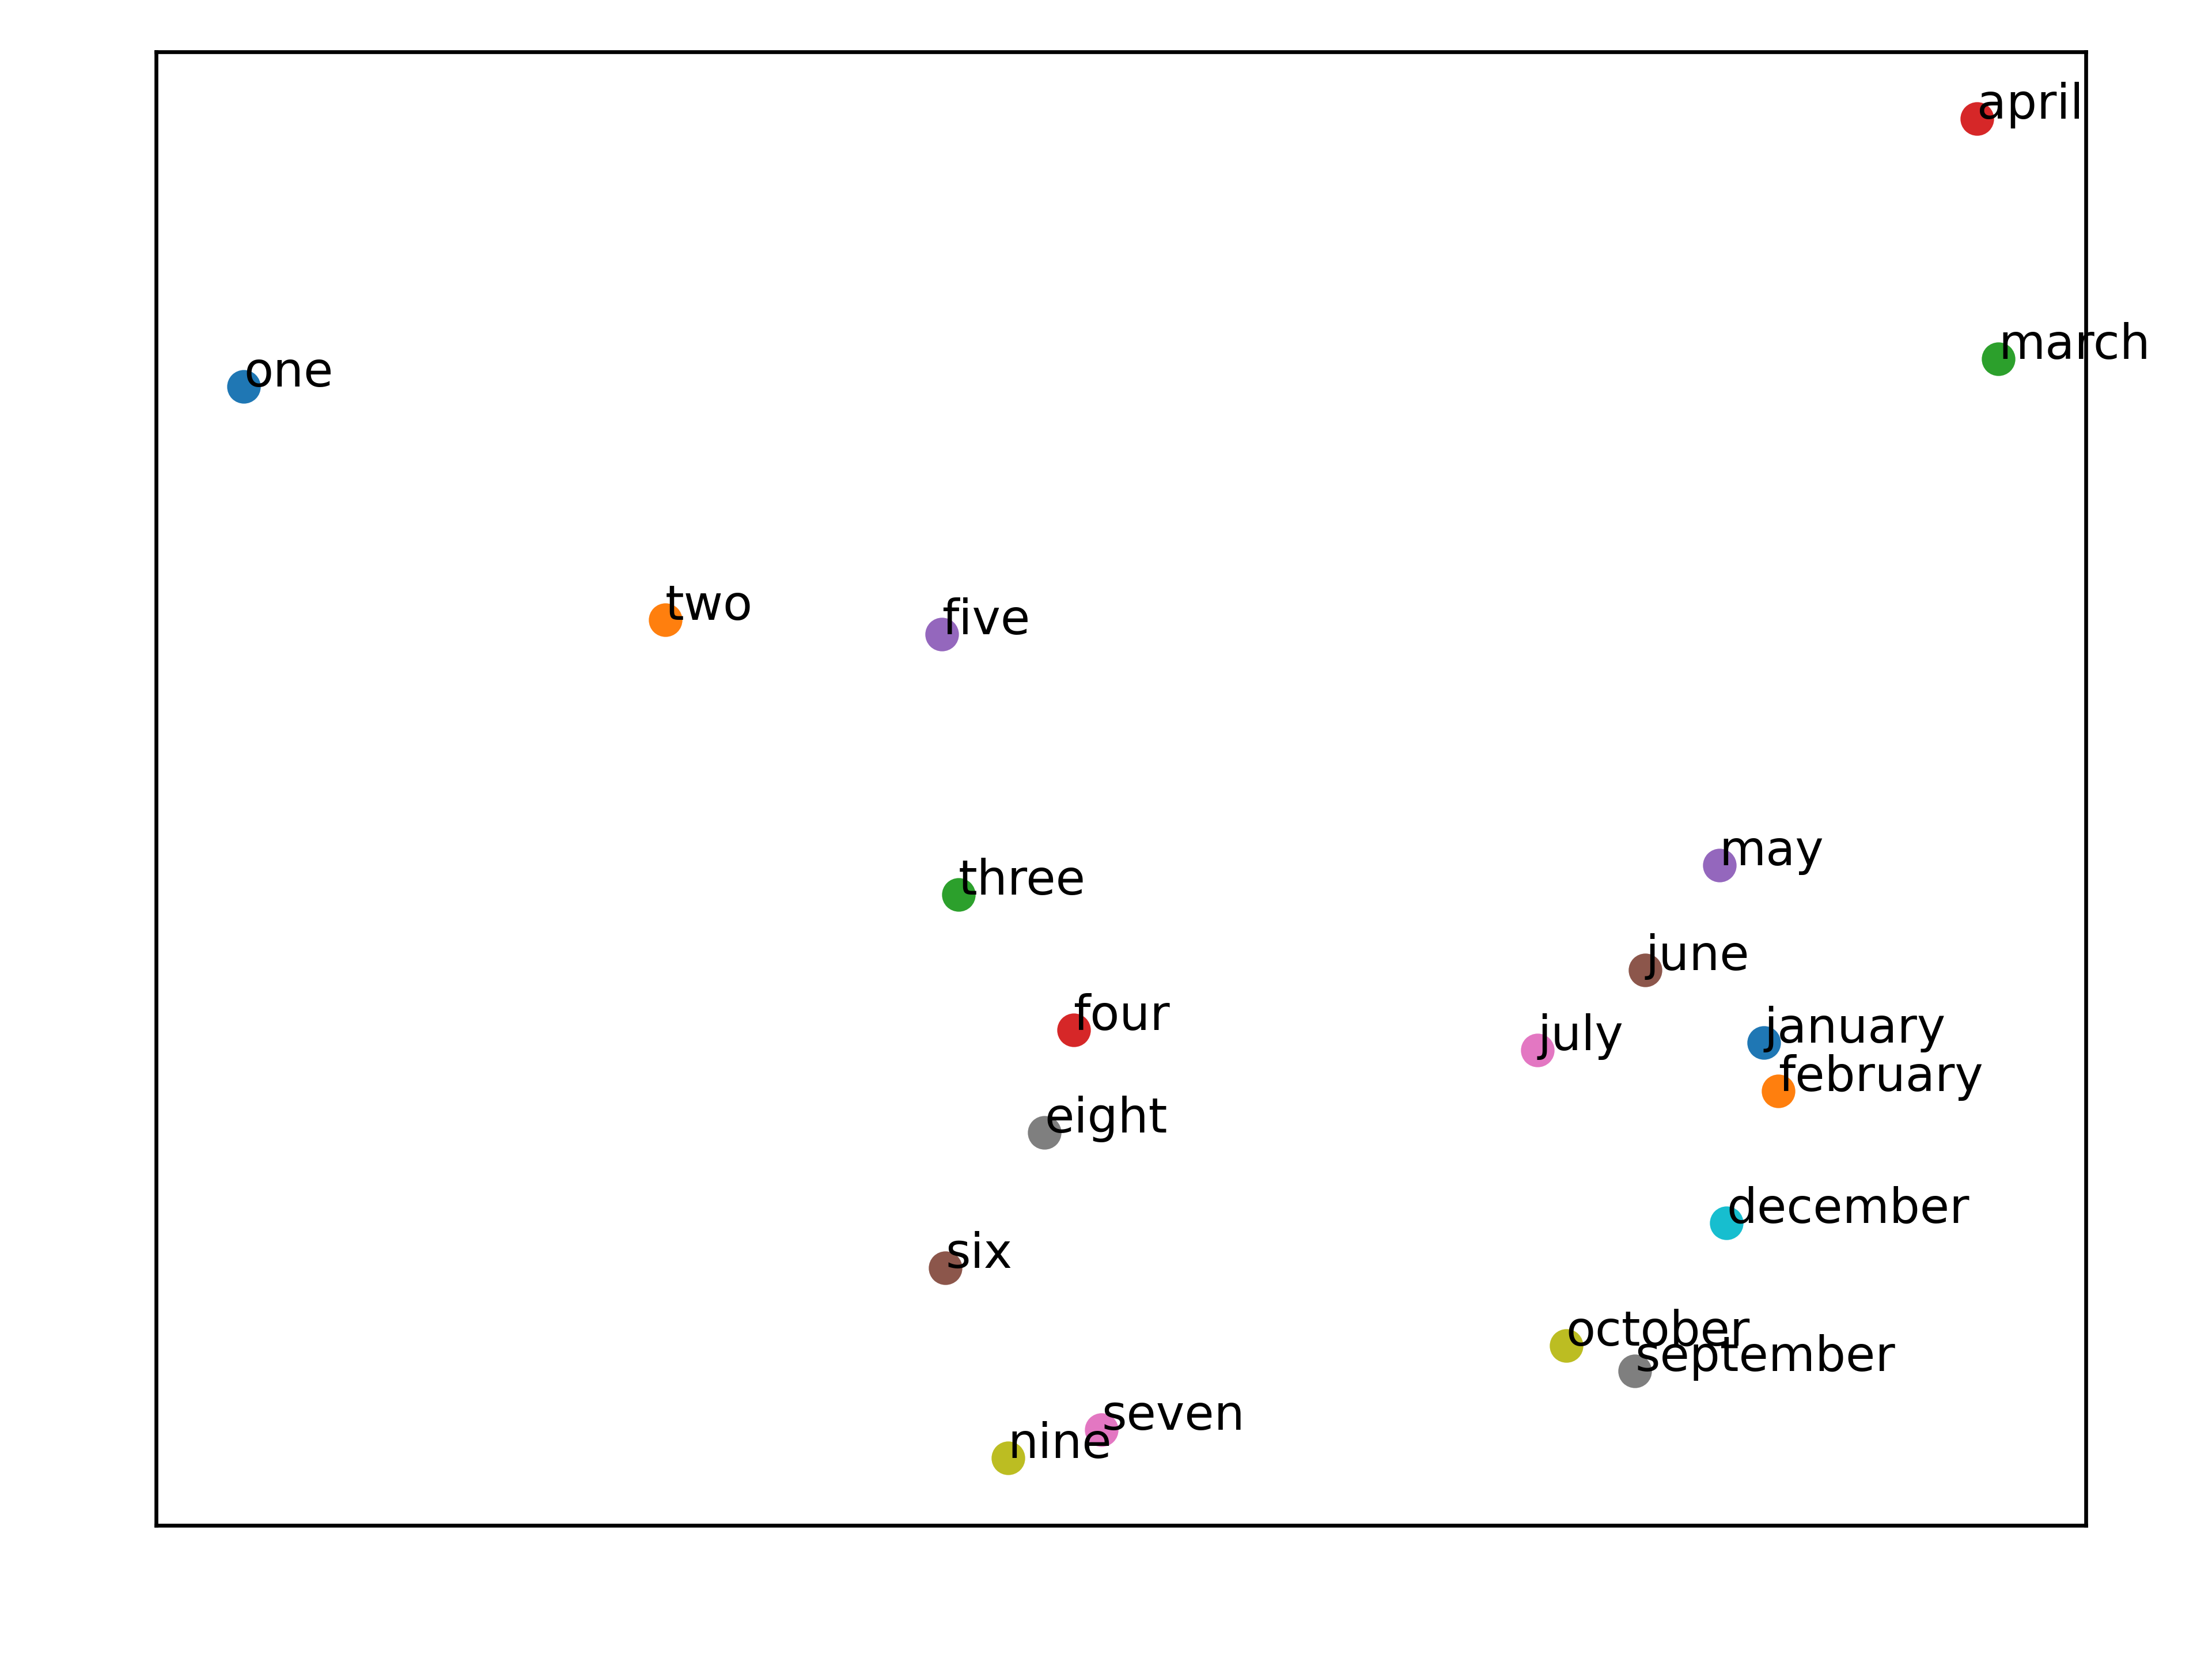
\includegraphics[scale=\myscale,scale=0.8]{figures/plongement-mots-1.png}
\end{center}
Les mots sont clairement séparés en deux catégories \og{}mois\fg{} et \og{}nombres\fg{} sans que l'on ait eu à définir une catégorie \og{}mois\fg{} ou \og{}nombres\fg{} (et sans même avoir construit le réseau pour cela).

Les plongements de \emph{BERT} ou \emph{GPT} sont évidemment bien plus performants.
Notre modèle est ici très simple, on le limite à un vocabulaire de $N=500$ mots, notre corpus n'est pas gigantesque et on ne tient compte que des paires de mots consécutifs. Mais même ainsi, on obtient des résultats intéressants.
\end{exemple}


\vfill
Vous trouverez des sites qui proposent de tester différents modèles en affichant de façon interactive les tokens et leur probabilité, par exemple :
  \mycenterline{\href{https://fr.vittascience.com/ia/}{fr.vittascience.com/ia/}}
\end{document}
